%%%%%%%%%%%%%%%%%%%%%%%%%%%%%%%%%%%%%%%%
%%%%%%%%%%%%%%%%%%%%%%%%%%%%%%%%%%%%%%%%
%%%%%
%%%%%  Préambule du document
%%%%%
%%%%%%%%%%%%%%%%%%%%%%%%%%%%%%%%%%%%%%%%
%%%%%%%%%%%%%%%%%%%%%%%%%%%%%%%%%%%%%%%%

%%%%%%%%%%%%%%%%%%%%%%%%%%%%%%%%%%%%%%%%
%%%%%  Reste à faire
%%%%%%%%%%%%%%%%%%%%%%%%%%%%%%%%%%%%%%%%

% Eléments certains :
%   Page titre à revoir
%   Présentation générale : faire une variante sobre et une variante bien moins sobre
%   Analyser les "\macro" trop longs et saut de ligne : le mbox
%   Utiliser biblatex
%   Détailler Beamer, longtable
%   Poursuivre tikz
%   Lister des grandes options de pstricks

% Maintenance :
%   Valider les liens web annuellement
%   Refaire Annexe A avec Installation de l'année en cours
%   Ajouter des erreurs au fur et à mesure

% Pistes :
%   Ajouter LyX ? Présenter LuaLaTeX ?
%   Présenter knitr (évolution de Sweave) ?


%%%%%%%%%%%%%%%%%%%%%%%%%%%%%%%%%%%%%%%%
%%%%%    Chaînes de compilation
%%%%%%%%%%%%%%%%%%%%%%%%%%%%%%%%%%%%%%%%

%%% Ce document est fourni avec les fichiers suivants :
%    - [chapitres]     : sous-répertoire contenant les fichiers tex des chapitres (17 fichiers) ;
%    - [figures]       : sous-répertoire contenant les figures (2 fichiers) ;
%    - [fontes]        : sous-répertoire contenant les fontes (4 fichiers) ;
%    - [images]        : sous-répertoire contenant les images (23 fichiers) ;
%    - [pagedegarde]   : sous-répertoire contenant les fichiers associés à pagedegarde (10 fichiers) ;
%    - bibliocours.bib : bibliographie associée à ce document ;
%    - cours.pdf       : le document final ;
%    - histogra.sty    : paquet présenté dans le cours ;
%    - lifecon.sty     : paquet présenté dans le cours ;
%    - pagedegarde.sty : paquet présenté dans le cours ;
%    - picins.sty      : paquet présenté dans le cours et parfois non installé ;
%    - plain-fr.bst    : format de bibliographie francisé ;
%    - styleindex.ist  : style des index ;

%%% Avec XeLaTeX + makeindex -> Attention à l'ordre des mots accentués en index.
% Ainsi \index{délimiteur} doit être mis à \index{delimiteur@délimiteur}
% (ce qui est fait ici mais doit donc être contrôlé si l'usage persiste.

% xelatex -synctex=1 -interaction=nonstopmode %.tex|bibtex %|makeindex -s styleindex.ist %.idx|makeindex -s styleindex.ist -o %.pnd %.pdx|makeindex -s styleindex.ist -o %.cnd %.cdx|xelatex -synctex=1 -interaction=nonstopmode %.tex|"C:/Program Files/Adobe/Reader 11.0/Reader/AcroRd32.exe" %.pdf

%%% Avec XeLaTeX + texindy

% xelatex -synctex=1 -interaction=nonstopmode %.tex|bibtex %|texindy -L french %.idx|texindy -L french -o %.pnd %.pdx|texindy -L french -o %.cnd %.cdx|xelatex -synctex=1 -interaction=nonstopmode %.tex|"C:/Program Files (x86)/Adobe/Reader 10.0/Reader/AcroRd32.exe" %.pdf


%%%%%%%%%%%%%%%%%%%%%%%%%%%%%%%%%%%%%%%%
%%%%%  Finies les blagues : du code !
%%%%%%%%%%%%%%%%%%%%%%%%%%%%%%%%%%%%%%%%

\documentclass[10pt,a4paper,oneside,french]{book}

\usepackage[body={15cm,23cm}]{geometry}
\usepackage[graph2,ps2,table2,index,symbs,maths,param]{styleyt}
\usepackage{fonctionscours}
\entetecours % Pour le format des en-têtes

% prerequis pythontex
\usepackage{fontspec}
\defaultfontfeatures{Ligatures=TeX}
\usepackage{pythontex}

%%%%%%%%%%%%%%%%%%%%%%%%%%%%%%%%%%%%%%%%
%%%%%  Informations générales
%%%%%%%%%%%%%%%%%%%%%%%%%%%%%%%%%%%%%%%%

\author{Yannick \textsc{Tanguy}}
\titre{P'tit cours de \LaTeX}
\version{2015-010}
\date{}


%%%%%%%%%%%%%%%%%%%%%%%%%%%%%%%%%%%%%%%%
%%%%%%%%%%%%%%%%%%%%%%%%%%%%%%%%%%%%%%%%
%%%%%
%%%%%  Le document
%%%%%
%%%%%%%%%%%%%%%%%%%%%%%%%%%%%%%%%%%%%%%%
%%%%%%%%%%%%%%%%%%%%%%%%%%%%%%%%%%%%%%%%

\makeindex
\begin{document}
\dominitoc                             % Déclenchement pour les mini-tables
\frontmatter                           % Numérotation spécifique des pages


%%%%%%%%%%%%%%%%%%%%%%%%%%%%%%%%%%%%%%%%
%%%%%  Page titre
%%%%%%%%%%%%%%%%%%%%%%%%%%%%%%%%%%%%%%%%

\begin{titlepage}
\begin{tikzpicture}[remember picture, overlay]
    \node at (current page.south west)
        {%
        \begin{tikzpicture}[remember picture, overlay]
            \node[inner sep=0cm] at (11,15) {
\includegraphics[height=35cm]{images/engrenage2.jpg}};
            \fill[bleu5](0,4.4) rectangle (10.7,5.4);
            \fill[bleu5](20.3,4.4) rectangle (21,5.4);
            \node at (15.5,4.5) {\resizebox{9cm}{!}{\fontfamily{lmr}\selectfont\Huge\LaTeX}};
            \node at (15.5,2.1) {\resizebox{5cm}{!}{\bfseries LE P'TIT COURS}};
            \node at (15.5,1.2) {\resizebox{2.5cm}{!}{\bfseries Y. Tanguy}};
        \end{tikzpicture}
        };
\end{tikzpicture}
\end{titlepage}


%%%%%%%%%%%%%%%%%%%%%%%%%%%%%%%%%%%%%%%%
%%%%%  Citation
%%%%%%%%%%%%%%%%%%%%%%%%%%%%%%%%%%%%%%%%

\citationseule{Encre n. : vil composé de tanin, de noir de fumée, de gomme arabique et d'eau, principalement utilisé pour faciliter la contagion de la bêtise et promouvoir le crime intellectuel.}{Ambrose}{Bierce}{The Devil's Dictionary}{1911}


%%%%%%%%%%%%%%%%%%%%%%%%%%%%%%%%%%%%%%%%
%%%%%  Introduction
%%%%%%%%%%%%%%%%%%%%%%%%%%%%%%%%%%%%%%%%

%%%%%%%%%%%%%%%%%%%%%%%%%%%%%%%%%%%%%%%%
%%%%%  Introduction
%%%%%%%%%%%%%%%%%%%%%%%%%%%%%%%%%%%%%%%%

\chapter{Avant de commencer}
\mtcaddchapter

{\bf \LARGE Hélas} pour vous, le rédacteur de ce qui suit avait envie de se manifester et de vous raconter \og sa vie, son \oe uvre \fg{} dans un subtil texte introductif. Cependant, pour des raisons manifestes de budget papier, votre serviteur a dû se limiter à la seule genèse de ce document. 

Lors de la première année de cette \og conférence \fg{} sur \LaTeX, un élève avait en effet suggéré qu'un polycopié compléterait le cours à merveille. Ce qui a donné ce que vous avez sous les yeux. Toutefois, l'idée à la base de ce document ne consiste pas à faire un parfait polycopié de cours de \LaTeX. Oh que non ! \`{A} cela deux raisons :

\begin{itemize}
\item sur l'Internet et en librairie existent d'excellents documents sur le sujet ; 
\item de façon plus pragmatique, votre rédacteur honni doit sacrifier son temps sur l'autel du travail et du roupillon crapuleux qui s'ensuit... ce qui lui laisse, hélas, fort peu de temps pour faire le polycopié ultime en 14 volumes. \\
\end{itemize}

L'idée qui sous-tend ce document est toute autre : vous disposez ici d'un \emph{exemple}, structuré en deux parties. La première partie revient à ce document final restituant nos choix de mise en forme. Le seconde partie est tout simplement le code source du document. Ce code utilise la plupart des notions et commandes présentées en y ajoutant à quelques reprises de légères subtilités pour les plus curieux d'entre vous. 

Par ailleurs, le peu d'exhaustivité de ce document est compensé à chaque fois que possible par des renvois à des documentations de référence (tel \paquet{minitoc}), des \href{http://fr.wikipedia.org/wiki/Hyperlien}{liens hypertexte}, de la bibliographie ou même des renvois à des pages de trois ouvrages de référence sous la forme suivante :
\incise{32--34,487--501}{24--47}{40--41}
Ces titres --- respectivement de Bernard \textsc{Desgraupes}\cite{desg}, Michel \textsc{Goossens}\cite{gomi} et Christian \textsc{Rolland}\cite{roll} --- sont référencés en bibliographie, en compagnie d'autres ouvrages traitant de \LaTeX, de typographie, de ponctuation \cite{coli} et même de couleur \cite{past} !

Bien évidemment, ce qui suit doit beaucoup aux nombreuses informations, aides et échanges trouvés sur l'Internet. Un grand merci aux passionnés de \LaTeX\ cachés derrière tout cela !


%%%%%%%%%%%%%%%%%%%%%%%%%%%%%%%%%%%%%%%%
%%%%%  Tables des matières
%%%%%%%%%%%%%%%%%%%%%%%%%%%%%%%%%%%%%%%%

\tableofcontents                       % Affichage de la table des matières
\listoftables
\listoffigures
\cleardoublepage                       % Permet de bien gérer la numérotation à placer
                                       % en face du \listof dans la table des matières.
\addcontentsline{toc}{chapter}{Liste d'exemples de code}
\listof{code}{Liste d'exemples de code}


%%%%%%%%%%%%%%%%%%%%%%%%%%%%%%%%%%%%%%%%
%%%%%  Coeur du document
%%%%%%%%%%%%%%%%%%%%%%%%%%%%%%%%%%%%%%%%

\mainmatter                            % Numérotation spécifique des pages (chiffres arabes depuis 1)
\part{Notions fondamentales}
%%%%%%%%%%%%%%%%%%%%%%%%%%%%%%%%%%%%%%%%
%%%%%  Chapitre Histoire
%%%%%%%%%%%%%%%%%%%%%%%%%%%%%%%%%%%%%%%%

\chapter{Une histoire de fous}
\mtcaddchapter

\section{Au commencement était \TeX} \index[con]{tex@\TeX!histoire}

\TeX\ (du grec $\tau \epsilon \chi$ qui a donné le mot \og technique \fg{} et qui explique la prononciation \og tèque \fg{}) est un programme de mise en forme de textes techniques, du simple article aux ouvrages en plusieurs tomes. Pour mieux comprendre l'aspect quasi-légendaire de \TeX, un peu d'histoire. 


\subsection{Le contexte}

Durant les années 70, Donald E. \textsc{Knuth}\cite{knut}, un mathématicien américain, s'était attelé à l'écriture de ce qui est désormais une référence fondamentale (rien de moins) en informatique : \emph{The Art of Computer Programming}. Dès l'origine, il avait planifié la sortie de plusieurs volumes sur une quarantaine d'années ! Or, en 1977, Donald \textsc{Knuth} rencontra un problème très particulier\footnote{Ce texte, maladroitement traduit par votre serviteur, a pour une source une conférence de Donald \textsc{Knuth} en 1986, reprise \emph{in extenso} dans le \href{http://www.tug.org/TUGboat/Contents/contents7-2.html}{septième numéro} de la revue TUGboat, page 95--98. \`{A} l'adresse \liensimple{ http://www.webofstories.com/play/17110?o=MS} se trouve une interview vidéo de Donald \textsc{Knuth} sur ce thème.}.

\begin{quotation} %\piccaption{Donald \textsc{Knuth}}
\parpic[r]{\fbox{\resizebox{3cm}{!}{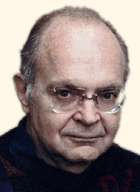
\includegraphics{images/Knuth.jpg}}}}\label{photoknuth} \og \emph{Pourquoi ai-je commencé à écrire \TeX\ en 1977 ? Cette histoire avait débuté longtemps auparavant, à l'occasion de la publication de mes livres \emph{The Art of Computer Programming}. J'avais préparé une seconde édition du tome 2, mais lorsque je reçus les épreuves, ce fut horrible --- la technique d'impression avait radicalement changé depuis la première édition. Les livres étaient maintenant composés à l'aide de photocomposeuses, au lieu des monotypes à plomb fondu ; en outre (hélas !), ces photocomposeuses étaient pilotées par des ordinateurs au lieu d'être supervisées \og manuellement \fg{}. Il en résultait une gestion désastreuse des blancs, surtout quand il s'agissait de mathématiques, et les fontes étaient décevantes comparées aux anciennes.} 

\emph{J'étais désespéré et ne savais que faire. \emph{Addisson-Wesley}\footnote{\'{E}diteur spécialisé dans les domaines scientifiques.} m'offrit de tout recomposer à l'aide des vieilles monotypes, mais je savais que la vieille méthode de composition était en train de mourir rapidement ; j'étais certain que lorsque j'aurai fini le tome 4, le même phénomène se reproduirait de nouveau et je ne voulais pas d'un résultat qui ressemblerait aux épreuves que j'avais vues. (...)} 
\end{quotation}

\begin{quotation}
\emph{Dès son début, en 1977, le projet de recherche \TeX\ dans lequel j'étais embarqué comportait deux axes principaux. Le premier était la qualité : nous ne voulions pas produire de bons documents, nous voulions qu'ils soient les meilleurs. (...)} 

\emph{Le second but recherché était l'archivage : il s'agissait de créer un système qui serait indépendant, autant que faire se peut, des mutations technologiques. Lorsqu'une nouvelle génération de machine à imprimer arriverait, je voulais être capable de maintenir le même niveau de qualité au lieu de repartir à zéro. Je voulais produire quelque chose qui pourrait encore servir dans un siècle. En d'autres termes, mon but était de m'y prendre de telle manière que, si l'on sauvegardait les spécifications d'un livre, nos descendants seraient encore capables d'éditer le même livre en l'an 2086.} \fg{}
\end{quotation}


\subsection{Le résultat}

La première version de \TeX\ date de 1978. Suite à corrections d'erreurs et à quelques évolutions, Donald \textsc{Knuth} décida de figer \TeX\ en 1982 à la version 3.14159\footnote{Chaque nouvelle version de \TeX\ ajoute des décimales de $\pi$ au numéro de version.}. 

En terme de qualité et conformément à l'idée initiale, \TeX\ a de quoi surprendre. Ainsi, son unité de longueur de référence la plus petite, le \emph{scaled point}, équivaut à $5,4\times10^{-9}$m. Autrement dit, les caractères sont ici placés avec une précision dépassant largement la précision de l'\oe il humain puisque nous nous plaçons ici à une échelle de l'ordre de grandeur du spectre de la lumière visible. \TeX\ sera donc dépassé quand l'évolution nous aura fait nous passer de nos yeux !

En terme informatique, \TeX\ est à la fois un programme et un langage. \TeX\ est ainsi un programme convertissant un fichier texte en un document décrivant la manière de positionner et de présenter ce texte sur une suite de pages. Par ailleurs, \TeX\ est un langage composé de plus de 300 fonctions dites \og primitives \fg{}. Ces fonctions, placées dans le fichier texte, permettent d'indiquer au programme \TeX\ comment présenter le texte. 

Ces fonctions, généralement simples, ont le désavantage de ne pas permettre de traiter un texte aisément. Seule l'action consécutive de plusieurs d'entre elles permet d'obtenir des résultats complexes, mais naturels. Ainsi en est-il, par exemple, de la création d'une page titre : dans ce cas, le texte sera centré selon plusieurs critères (le format de la page en particulier), sera écrit plus grand, sera sur une feuille séparée des autres, feuille qui ne sera pas numérotée... De fait, \TeX\ permet de créer une nouvelle fonction de présentation par composition de fonctions primitives : une \terme{macrocommande} ou macros, nommées dans toute la suite commandes. Bien entendu, de nouvelles commandes peuvent également s'obtenir par composition de commandes existantes.

Un ensemble de commandes pensées pour permettre de présenter un document forme un sur-ensemble de \TeX, un \terme{format}. Le premier format créé par \textsc{Knuth}, un format minimal, s'appelle \emph{plain}.  


\section{Puis vint \LaTeX}

\parpic[r]{\fbox{\resizebox{3cm}{!}{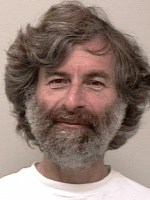
\includegraphics{images/Lamport.jpg}}}}
\LaTeX\ (prononcé \og latèque \fg{}), écrit en 1982 par Leslie \textsc{Lamport} \cite{lamp}, est un format simplifiant l'usage de \TeX\ en le dotant de commandes exécutant des tâches importantes de présentation. 

Par la suite, des ensembles de commandes ont été développés, ceci afin de développer tel ou tel aspect particulier de présentation : par exemple offrir des mises en page alternatives des titres. Un tel ensemble de commandes regroupées en un fichier est ici appelé une \terme{extension} ou un \og \terme{paquet} \fg{} (en anglais \emph{package}). 

Et les besoins d'extension étaient vastes ! Les possibilités de \TeX\ par le biais de \LaTeX\ et de ses extensions ont, de fait, explosé. D'un logiciel pensé pour écrire des articles scientifiques assez stéréotypés, \TeX\ est devenu un logiciel pensé pour rédiger des documents très variés --- de la simple lettre au livre en passant par les transparents ou des partitions --- dans des domaines aussi différents que la physique, la chimie, les mathématiques, la linguistique, la musique, le jeu d'échecs, etc. 

Depuis 1994, la version normalisée s'appelle \LaTeXe{} (qui se lit \og latèque deux oeufs \fg{}). Elle est compatible (dans la mesure du possible) avec les anciens standards.


\section{Longtemps après vinrent \XeTeXtitre et \XeLaTeXtitre}

\parpic[r]{\fbox{\resizebox{3cm}{!}{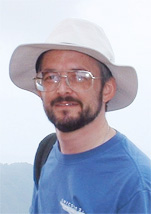
\includegraphics{images/Kew.jpg}}}}
\TeX\ et \LaTeX\ sont rapidement devenus des outils internationaux mais ils avaient quelques limitations, en particulier sur la gestion de langues étrangères et de polices de caractères. Ceci s'expliquait en particulier par une problématique d'encodage que Jonathan \textsc{Kew}, avec \XeTeX, fit grandement avancer.

Fondamentalement, les ordinateurs ne traitent que des nombres binai\-res. Un fichier texte ne contient pour ainsi dire qu'une chaîne de zéros et de uns. Pour que l'ordinateur nous restitue des caractères, il faut avoir recours à un \terme{encodage} autrement dit une table de correspondance qui permet de dire que telle chaîne binaire est associée à tel caractère unique. Par exemple, en encodage ASCII, \og 01000001 \fg{} correspond à la lettre \og A \fg{}. 

Cependant, il existe plusieurs encodages et ils ne sont pas forcément cohérents entre eux. Depuis 1991, un projet d'encodage mondial suit cependant son cours : Unicode\footnote{Le site officiel d'Unicode présente très largement cet encodage : \liensimple{http://www.unicode.org/}.}. Il a pour but de traiter les différents langues de l'humanité en un unique encodage : s'y retrouvent des langues aussi variées que le japonais, le tamul, le tagalog, le khmer.% de fait, des caractères aussi différents que ȹ, Җ, څ , ௸, ⾦. 

Du fait de ses travaux l'amenant à travailler avec des langues asiatiques, Jonathan \textsc{Kew}\footnote{Une interview de Jonathan \textsc{Kew} sur ce sujet : \liensimple{http://tug.org/interviews/kew.html}.} proposa en 2004 une version de \TeX, nommée \XeTeX\ (prononcé \og zétex\fg), permettant de gérer l'Unicode et donc le multilinguisme.

\XeTeX\ et \paquet{fontspec} --- un paquet dédié à la gestion des polices de caractères --- offrent en plus des fonctionnalités plus étendues (voir page~\pageref{fontes}) :
\begin{itemize}
\item accès généralisé aux polices OpenType Fonts (OTF) et TrueType Fonts (TTF) ;
\item accès à des caractères alternatifs et à des ligatures spécifiques de ces polices ;
\item gestion de la transparence des caractères ;
\item simplification de la chaîne de compilation pour \paquet{pstricks}.
\end{itemize}

\section{Et \LuaTeXtitre et \LuaLaTeXtitre les rejoignirent}

Développé par Taco \textsc{Hoekwater}, Hartmut \textsc{Henkel} et Hans \textsc{Hagen}, \LuaTeX\footnote{Le site officiel est à l'adresse \liensimple{http://luatex.org/}.} étend les possibilités du monde \TeX\ dans une nouvelle direction : intégrer un langage de script, Lua, dans le code \TeX. Ceci permet de faire exécuter à \LaTeX\ par le biais de Lua des tâches plus complexes dans le traitement du texte : Lua peut en effet modifier le comportement de \TeX\ ou le compléter. De façon similaire, ceci permet de faire des calculs complexes avec \TeX, ce dernier étant relativement limité en ce domaine.

\section{Un souci}

L'actuelle variété du monde de \TeX\ a tout de même un prix dans la mesure où ces extensions et différentes versions de \TeX\ ont introduit des incompatibilités : différents paquets utilisent des noms de commandes identiques pour réaliser des tâches bien différentes. Du coup, une certaine prudence reste parfois de mise si de multiples paquets sont utilisés, ceci pour éviter des résultats erronés. 

Cette situation a conduit au projet de normalisation \LaTeX3, sous la direction des \og gurus \fg{} \LaTeX\ parmi lesquels se trouve Leslie \textsc{Lamport}\footnote{Pour plus de détails, consulter \liensimple{http://www.latex-project.org}.}. L'histoire n'a donc pas fini de se poursuivre !


\begin{flushright}
Vous cernez mieux la bête ? Passons alors à la \TeX nique !
\end{flushright}
%%%%%%%%%%%%%%%%%%%%%%%%%%%%%%%%%%%%%%%%
%%%%%  Chapitre Fonctionnement
%%%%%%%%%%%%%%%%%%%%%%%%%%%%%%%%%%%%%%%%

\chapter{Le fonctionnement de \TeX}
\mtcaddchapter

Décrire le fonctionnement précis et exact de \TeX, le programme derrière le format \LaTeX, demanderait un ouvrage complet. En l'occurrence, cet ouvrage existe et s'appelle le \TeX book\cite{knut} : il a été rédigé par \textsc{Knuth} lui-même... un expert que nous ne chercherons pas à dépasser sur son sujet ! Nous nous limitons donc ici à une description partielle et partiale de la structure d'un document \LaTeX, de sa composition et des conséquences de ces règles sur la façon de rédiger du code \LaTeX\footnote{Pour simplifier, \TeX\ et \LaTeX\ seront systématiquement confondus par la suite.}.


\section{Un fichier \LaTeX}

Un fichier \LaTeX\ est un document lisible par n'importe quel éditeur de texte classique. Le texte et les commandes --- toute chaîne de caractères commençant par un \og \macro{} \fg{} --- qui y sont inclues restent lisibles, ceci en opposition avec de nombreux autres logiciels qui codent ces éléments. 

Un fichier \LaTeX\ a pour extension \dextension{tex}\footnote{Dans toute la suite, un \og fichier d'extension tex \fg{} sera désigné comme \og fichier \dextension{tex} \fg{}.} et son nom ne doit pas contenir d'espace ou de lettre accentuée. Il est traditionnellement dénommé fichier source ou \terme{source}\footnote{Source est de plus en plus considéré comme un nom masculin dans ce cas précis.}, pour le distinguer du fichier présentant le résultat final.



\subsection{La structure}

Ce fichier est toujours constitué de deux parties : 
\begin{itemize}
\item le \terme{préambule}, situé en début de document. Il contient un ensemble de définitions génériques servant à présenter l'ensemble du document. Plus précisément, s'y trouvent réunis la définition du type de document, l'appel à des paquets spécifiques --- fichiers définissant des commandes étendant les fonctionnalités de \LaTeX\ --- mais aussi la (re)définition de commandes spécifiques au document. Placer du texte libre dans cette partie provoque une erreur de \LaTeX ; 
\item le \terme{corps}. Il contient le texte qui sera affiché ainsi que des commandes modifiant la présentation de ce texte à l'endroit où elles sont placées ou sur la zone qu'elles encadrent. \\
\end{itemize}

Les deux parties sont séparées par la commande\footnote{L'usage de la fonte \og machine à écrire \fg{} est quasiment systématique dans les ouvrages d'informatique lorsque est évoqué un élément du langage de programmation, élément qui serait tapé tel quel à l'écran. Est ici ajouté de la couleur pour le plaisir de complexifier les définitions des commandes permettant cet affichage.} : \macro{begin\{document\}}. Le corps s'achève avec la commande \macro{end\{document\}}. Tout le texte placé au-delà de cette seconde instruction est purement et simplement ignoré par \LaTeX.


\subsection{Un exemple}

Voici un exemple simple d'un fichier \LaTeX\ : 

\begin{codesimple}{Exemple simple}{exemplesimple}
\documentclass[a4paper]{article}
\usepackage{eurosym}
\begin{document}
Savais-tu que le signe de l'\emph{euro} se tape \euro ?
\end{document}
\end{codesimple}

Ici, le préambule se limite à deux lignes. La première ligne définit le type du document : elle demande à \LaTeX\ de faire appel à des fichiers contenant des commandes et paramètres permettant de présenter le document. Ce point est détaillé au chapitre~\ref{classe}.

La seconde ligne charge un paquet\footnote{Dans toute la suite, les paquets seront indiqués avec ce code visuel.}, \paquet{eurosym}, qui définit la commande \macro{euro}.

Dans le corps, constitué des trois lignes suivantes, se trouve le texte à afficher. Ce texte est localement modifié par la commande \macro{emph} qui fait passer le texte qu'elle contient entre accolades en italique. De plus, la commande \macro{euro} va permettre l'affichage du symbole \euro.


\section{La \og grammaire \fg{} de \LaTeX}
\subsection{Les caractères actifs} \incise{15,53}{---}{14}

Les règles du langage \LaTeX\ se centrent sur l'usage de caractères spécifiques dit \og caractères actifs \fg.

\begin{table}[!ht]
\begin{tablecouleur}
\begin{tabular}{cm{10cm}}
\rowcolor{bleu20}
\color{white}\bf Caractères		& \multicolumn{1}{c}{\color{white}\bf Utilisation}
\\
\macro{}	& Il indique le début d'un nom de commande : \LaTeX\ exécute alors les tâches associées au nom de la commande. 
\\ 
\macron{\{} 	\macron{\}} & Toujours par couple, elles encadrent et isolent des ensembles spécifiques, d'où leur nom de \textbf{délimiteur}\index[con]{delimiteur@délimiteur}.%\terme avec texindy directement.\newcommand{\terme}[1]{\textbf{#1}\index[con]{#1}}
\\ 
\macron{\%} 	& Il indique que ce qui le suit est un commentaire. Jusqu'au prochain passage à la ligne, \LaTeX\ ignore ce qui est écrit et ne l'affiche pas.
\\ 
\macron{\$} \macron{\_} \macron{\^{}} & Ils participent à la rédaction de mathématiques. Voir page \pageref{mathématique}.
\\ 
\macron{\&}  & Il participe à la constitution des tableaux. Voir page \pageref{tableau}.
\\ 
\macron{\#}  & Il participe à la définition de nouvelles commandes. Voir page \pageref{definition}.
\\ 
espace & Plusieurs espaces consécutives valent une seule espace.
\\ 
retour à la ligne & Un retour à la ligne est considéré comme une espace. Deux retours à la ligne consécutifs ou plus comme un seul et unique changement de paragraphe.
\\ 
\macron{@} & Très particulier, il peut être activé pour devenir un caractère utilisable dans les noms de commandes en programmation avancée, ceci avec l'utilisation de \macro{makeatother} (activation) et de \macro{makeatletter} (désactivation).
\\ 
\end{tabular}
\end{tablecouleur}
\caption{Caractères actifs}\label{tablecaracteresactifs}
\end{table}

En programmation avancée, ces caractères peuvent être remplacés par d'autres ou redéfinis pour se voir attribuer d'autres rôles. Qui serait intéressé par ce point doit faire une recherche sur la notion de \terme{catcode}, ou code de catégorie (de caractère)\footnote{Par exemple : \liensimple{http://www.math.u-psud.fr/~bernardofpc/ens/CIES/Avance.pdf}.} profondément lié à la manière dont \LaTeX\ lit un document.

L'affichage de tels caractères actifs dans le texte final (ne serait-ce par exemple que pour les citer dans le tableau ci-dessus) s'obtient par le recours à des commandes présentées dans la table \ref{tablecaracteres}, page~\pageref{tablecaracteres}. \label{monexemple}


\subsection{Les groupes}

Pour que \LaTeX\ puisse présenter un endroit spécifique d'un document, il lui faut savoir quel est l'état des différentes valeurs des paramètres de présentation : fonte à utiliser, format de la page et ainsi de suite. Pour cela est utilisée la notion de \terme{groupe}. Un groupe est au sens le plus large une zone de notre document. Un groupe peut être délimité de deux façons : 
\begin{itemize}
\item par des accolades ouvrantes et fermantes ;
\item par des crochets ouvrants et fermants quand ils servent à indiquer un argument d'une commande ;
\item par des commandes d'environnement, telles \macro{begin\{document\}} et \macro{end\{document\}}, présentées ci-après.  
\end{itemize}

Un groupe peut contenir d'autres groupes (des sous-groupes) et ainsi de suite. En terme d'état, chaque sous-groupe récupère l'état du groupe au moment où il est ouvert. Cet état initial peut ensuite être librement modifié dans le sous-groupe. Cependant, lorsqu'un sous-groupe s'achève et que \LaTeX\ revient dans le groupe, il reprend l'état qu'avait le groupe, indépendamment de tous les changements apportés par le sous-groupe. 

L'exemple ci-dessous montre ce principe avec deux commandes opérant un changement de présentation du texte à partir du moment où elles apparaissent dans le texte : \macro{itshape} fait passer le texte en italique, \macro{upshape} le fait passer en caractères droits (dits romains).

\begin{codedouble}{Exemple de groupe}{exemplegroupe}
Voici un {exemple \itshape de {\upshape texte illustrant les} groupes} 
sous \LaTeX.
\end{codedouble}

Ici, dans le groupe initial, \LaTeX\ rédige en caractères romains. Lorsqu'il passe dans le sous-groupe, il garde ce réglage jusqu'à rencontrer \macro{itshape} qui le fait passer à l'italique. Lorsqu'il passe dans le sous-sous-groupe, il reçoit immédiatement la consigne de passage en caractères droits. En l'absence d'autres réglages, ce format perdure jusqu'à la fin du sous-sous-groupe. Lorsque \LaTeX\ quitte cette zone, il revient au sous-groupe avec sa présentation italique. Le mot \og groupes \fg{} est donc en italique. De même, une fois qu'il quitte le sous-groupe, il revient au réglage qu'avait le groupe : l'écriture en romain.


\subsection{Les différentes commandes}

\LaTeX\ distingue tout d'abord lettres majuscules et minuscules\footnote{\LaTeX\ est dit \og sensible à la casse \fg{}.}: la commande \macro{Test} peut avoir une définition différente de la commande \macro{test} comme de la commande \macro{TesT}. 

Les commandes sont parfois dotées d'arguments. Ceux-ci sont placés immédiatement après le nom de la commande, sans espace : ils sont le plus souvent introduits par des \macron{\{} lorsqu'ils sont obligatoires, par des \macron{[}\footnote{Les crochets ne sont pas considérés comme des caractères actifs, contrairement aux accolades.} lorsqu'ils sont facultatifs et conclus respectivement par des \macron{\}} et des \macron{]}. De fait, un argument est un groupe.

Trois grands types de commandes coexistent :
\begin{itemize}
\item la commande simple avec arguments sous la forme usuelle \macro{macro\{{\it arg1}\}...\{{\it argN}\}}. Elle exécute normalement une action à l'endroit où elle se trouve dans le texte et agit sur ou avec ses arguments. Par exemple,  \macro{textbf\{{\it texte}\}} mettra le texte en argument en gras. Les arguments ont des tailles limitées à un paragraphe au plus.
\item la commande \terme{bascule}, le plus souvent sans argument. Celle-ci modifie le comportement de \LaTeX\ jusqu'à la fin du groupe dans lequel elle se situe. Par exemple, \macro{bfseries} fait que le texte qui suit s'écrit désormais en gras. 
\item la commande \terme{environnement} de la forme \macro{begin\{{\it environnement}\}} toujours suivie plus loin de la nécessaire fin\footnote{Sous peine d'obtenir une erreur de \LaTeX\ !} \macro{end\{{\it environnement}\}}. La zone délimitée par ces deux commandes, qui peut contenir de nombreux paragraphes, est alors modifiée. Ainsi, l'environnement \macron{center} va centrer tout le texte placé entre les deux commandes.
\end{itemize}

Dans la suite, ces différentes variantes seront respectivement appelées commandes, bascules et environnements.

\subsection{Unités de mesure}\label{unite}

Parmi les arguments qui peuvent être communiqués à des commandes \LaTeX\ se trouve des longueurs. Ces  commandes permettent le plus souvent de faire des réglages, par exemple insérer à la fin de cette phrase une espace de 2cm\hspace*{2cm}. 

Les unités de longueur absolues connues par \LaTeX\ sont :

\begin{table}[!ht]
\begin{tablecouleur}
\begin{tabular}{cccc}
\rowcolor{bleu20}
\color{white}\bf Unité		& \color{white}\bf  Nom		& \color{white}\bf Définition & \color{white}\bf	Mesure (en mm) \\ 
cm				& centimètre							&	1 cm = 0,01 m	& 10 mm 		\\
mm				& millimètre							&	1 mm = 0,1 cm	& 1 mm			\\
in				& pouce (\emph{inch})					&	1 in = 2,54 cm 	& 25,4 mm		\\
bp				& gros point (\emph{big point})			&	72 bp = 1 in 	& 0,3527778 mm	\\
pt				& point                					&	72,27 pt = 1 in & 0,3514598 mm 	\\ 	
pc				& pica 									&	1 pc = 12 pt 	& 4,2175176 mm	\\ 
dd				& point didot							& 1157 dd = 1238 pt & 0,3760650 mm  \\
cc				& cicéro								&	1 cc = 12 dd 	& 4,5127803 mm  \\
sp				& point d'échelle (\emph{scaled point})	& 65536 sp = 1 pt	& 0,0000054 mm\\
\end{tabular}
\end{tablecouleur}
\caption{Unités de longueur absolues} \label{unitesabsolues}
\end{table}

Par ailleurs, \LaTeX\ peut manipuler des longueurs relatives, autrement dit des longueurs qui dépendent de la taille de certains caractères de la police courante. Il existe pour cela deux unités :

\begin{table}[!ht]
\begin{tablecouleur}
\begin{tabular}{cc}
\rowcolor{bleu20}
\color{white}\bf Unité		& \color{white}\bf  Nom					\\ 
em							& cadratin (largeur de la lettre M)		\\ 	
ex							& hauteur d'x							\\ 
\end{tabular}
\end{tablecouleur}
\caption{Unités de longueur relatives} \label{unitesrelatives}
\end{table}

Pour être complet, \LaTeX\ admet également des longueurs élastiques\footnote{Elles ne sont qu'évoquées ici mais sont largement développées dans le cours avancé de Manuel \textsc{Pégourié-Gonnard} \cite{pego}. Ces définitions sont également vues dans l'annexe C en ligne de \cite{bito} : \liensimple{http://latex-pearson.org/ressources/2010/annexe-C.pdf}.} qui se présentent à titre d'exemple sous la forme suivante : \macron{1cm plus 1ex minus 2mm}. Dans cet exemple, la longueur est comprise entre 1cm$-$2mm et 1cm$+$1ex selon les contraintes présentes ; 1cm est la longueur en l'absence de contraintes.

\section{La compilation}\label{compilation}\index[con]{compilation} \incise{19--30}{---}{7--12} 

Pour obtenir le document mis en forme, il faut effectuer une \terme{compilation} du fichier \dextension{tex}, autrement dit le faire lire et retranscrire par \LaTeX\ en un document d'un autre format qui nous donnera l'affichage souhaité, généralement un fichier \dextension{dvi} ou un fichier \dextension{pdf}. 


\subsection{La mécanique de la compilation}

Lors de la compilation, \LaTeX\ analyse et transforme les différentes commandes en une suite de fonctions fondamentales qui lui dictent la manière de présenter les pages de texte. Au fur et à mesure, selon les règles usuelles et les modifications apportées parfois par les commandes, \LaTeX\ prépare des boîtes contenant des caractères puis des boîtes contenant des boîtes de caractères autrement dit des boîtes-mots, puis des boîtes-lignes puis des boîtes-paragraphes. \`A chaque étape, il prépare également les espaces entre les boîtes selon des règles typographiques\footnote{Entre autres, la règle de césure qui distingue \LaTeX\ d'autres logiciels.} ou des règles imposées par les commandes. 

Cet empilement de boîtes finit par générer une page. Une fois une page générée, \LaTeX\ passe à la suivante et ne revient pas en arrière.

De ce fait, \LaTeX\ ne peut créer directement des éléments demandant une vision de tout le document : une table des matières, un index ou un renvoi vers une page. Pour obtenir de tels éléments, il faudra compiler deux ou trois fois le document, \LaTeX\ réutilisant des informations stockées par la dernière compilation dans des fichiers annexes prévus pour ce type de fonctionnalités.


\subsection{Les fichiers générés par la compilation}

La compilation produit plusieurs fichiers, chacun ayant un rôle spécifique pour l'utilisateur et pour \LaTeX\ :
\begin{itemize}
\item le fichier \dextension{dvi}\footnote{DVI signifie \og DeVice-Independant \fg{} soit \og indépendant du type d'unité ou du périphérique \fg{}.}, un fichier qui restitue un document finalisé.
\item le fichier \dextension{log}, ou \terme{journal}. Il contient des informations sur le travail effectué lors de la compilation.  
\item le fichier \dextension{aux}, ou \og auxiliaire \fg{}. Il contient des informations de compilation que \LaTeX\ réutilise lors de la compilation suivante. Parmi celles-ci, se trouvent des informations sur les références dans le document, des numéros de pages, des éléments servant à la table des matière.
\item et parfois d'autres fichiers en cas d'utilisation de commandes ou de paquets spécifiques. Par exemple, le paquet \paquet{minitoc} génère de nombreux fichiers \dextension{mtc} (suivis de chiffres).
\end{itemize}


\section{La gestion des erreurs}
\incise{29--30}{---}{187--200}

L'erreur est hélas humaine... et \LaTeX\ déteste les erreurs. Les erreurs interfèrent avec la compilation et génèrent souvent une restitution partielle du fichier \dextension{dvi}. \LaTeX\ peut en effet s'arrêter en cours de compilation si les erreurs sont trop importantes.

Dans ces cas-là, il est recommandé de regarder le fichier journal. Ce fichier contient souvent l'information de la ligne où est survenue l'erreur et assez fréquemment sa raison : une commande inconnue, une accolade oubliée, des mathématiques mal tapées. Ce fichier est donc d'une aide précieuse, quoique rédigé en anglais. La plupart des éditeurs \LaTeX\ permettent d'ailleurs de visionner ce fichier lors de la compilation pour comprendre et corriger les erreurs.

Pour sauver le commun des mortels de certaines erreurs assez complexes, l'annexe \ref{erreur} a été constituée sur ce sujet, page \pageref{erreur}.


\section{L'impression} \incise{22}{---}{12--14}

Le fichier \dextension{dvi}, s'il peut être visualisé, ne peut être imprimé directement. Il faut le convertir en un autre format et, pour cela, utiliser un programme extérieur à \LaTeX. De façon courante, il est converti à l'aide du programme \programme{dvips} en document postscript (dit fichier \dextension{ps}) lisible et imprimable. Ceci permettra d'utiliser certains paquets spécifiques présentés en section \ref{pstricks}. Qui plus est, un document \dextension{ps} peut être  converti en \dextension{pdf}. Un second programme de conversion est ici utilisé : \programme{ps2pdf}.

\section{Des compilations alternatives}\label{compilations}

La compilation décrite jusqu'ici de base sur la mécanique historique. Les variantes de \LaTeX\ ont revu cette mécanique et l'ont simplifié.

Ainsi, il est possible d'utiliser le programme \programme{pdflatex} qui génère directement un fichier \dextension{pdf} à partir du fichier \dextension{tex}. S'il présente des incompatibilités avec certaines des fonctionnalités vues dans la suite de ce cours, essentiellement le paquet \paquet{pstricks}, ce programme autorise en contrepartie l'insertion des images \dextension{jpg}.

Il est également possible de retenir pour la compilation les programme \programme{xetex} ou \programme{lualatex}. Ils permettent de la même manière de passer du fichier \dextension{tex} au fichier \dextension{pdf}. Toutefois, ces programmes demandent d'appliquer un encodage différent au fichier source et il implique de placer un préambule différent de celui utilisés normalement avec \LaTeX. Ces points sont présentés en page \pageref{xelatex}.

La figure suivante résume l'ensemble de ces processus.

%%%%%%%%%%%%%%%%%%%%%%%%%%%%%%%%%%%%%%%%
%%%%%  Figure : tex -> pdf
%%%%%%%%%%%%%%%%%%%%%%%%%%%%%%%%%%%%%%%%

% Ce code demande des définitions (fleche, flechetiret..) défini 
% dans fonctionscours.sty (partie "Code TIKZ pour des figures")

\begin{figure}[H]
\centering
\begin{tikzpicture}
% Principaux objets
\tzfichier(0,5)(tex)
\tzfichier(5,5)(dvi)
\tzfichier(5,3)(log)
\tzfichier(5,1)(aux)
\tzfichier(10,5)(ps)
\tzfichier(10,1)(pdf)
\tzprogramme[](2.5,5)(latex)
\tzprogramme[](7.5,5)(dvips)
\tzprogramme[](10,3)(ps2pdf)
\tzprogrammelong[color=orange3](0,2.8)(pdflatex)(\programme{pdflatex} ou \programme{xelatex} ou \programme{lualatex}) % 2.8 pour alignement.

% Lieux pour éviter des confusions de flêches.
\node[gauche] (pdflatex1) at (pdflatex.south){};
\node[droite] (pdflatex2) at (pdflatex.south){};
\node[dessus]   (log1) at (log.west){};
\node[dessous]  (log2) at (log.west){};
\node[dessus]   (aux1) at (aux.west){};
\node[dessous]  (aux2) at (aux.west){};
\node[dessus]   (aux3) at (aux.east){};
\node[dessous]  (aux4) at (aux.east){};

% Flêches de tex vers pdf
\draw[fleche,>-] (tex.east) -- (latex.west);
\draw[fleche] (latex.east) -- (dvi.west);
\draw[fleche,>-] (dvi.east) -- (dvips.west);
\draw[fleche] (dvips.east) -- (ps.west);
\draw[fleche,>-] (ps.south) -- (ps2pdf.north);
\draw[fleche] (ps2pdf.south) -- (pdf.north);

% Flêches de tex vers log/aux et flêche retour 
\draw[fleche] (latex.east) -| (3.9,4) |- (log1);
\draw[fleche] (latex.east) -| (3.9,4) |- (aux1);
\draw[fleche,>->] (aux3) -| (6.1,0.5) |- (5,-0.2) -| (latex.south);

% Flêches de tex vers pdflatex puis pdf
\draw[flechetiret,>-] (tex.south) -- (pdflatex.north);
\draw[flechetiret] (pdflatex1) |- (6,-1) -| (pdf.south);

% Flêches de pdflatex vers log/aux et flêche retour
\draw[flechetiret] (pdflatex.east) -- (log2);
\draw[flechetiret] (pdflatex.east) -| (3.5,2) |- (aux2);
\draw[flechetiret,>->] (aux4) -| (6.5,0.5) |- (3,-0.6) -| (pdflatex2);

\end{tikzpicture}
\caption{Du fichier \dextension{tex} au fichier \dextension{pdf}}
\end{figure}

\part{Notions courantes}
%%%%%%%%%%%%%%%%%%%%%%%%%%%%%%%%%%%%%%%%
%%%%%  Chapitre Préambule et classe
%%%%%%%%%%%%%%%%%%%%%%%%%%%%%%%%%%%%%%%%

\chapter{Préambule et classe du document}
\mtcaddchapter

\label{classe}
\section{Un préambule minimal} \incise{31--36}{17--20}{39--41}

Le préambule varie selon la chaîne de compilation qui a été choisie.

\subsection{Cas avec \LaTeX\ et pdf\LaTeX}

Un document en français devrait toujours contenir au moins les commandes suivantes :

\begin{codesimple}{Un code minimal pour \LaTeX}{codeminimum}
\documentclass[§oc£¤options§fc]{§oc£¤classe§fc}
\usepackage[frenchb]{babel}
\usepackage[T1]{fontenc}
\usepackage[latin1]{inputenc}
\usepackage{lmodern}  
\begin{document} 

\end{document}
\end{codesimple}

Le chargement des paquets \paquet{fontenc} et \paquet{inputenc} font appel à la notion d'encodage. Nous nous contenterons d'indiquer que l'appel du paquet \paquet{fontenc} avec l'option \vue{T1} permet à \LaTeX\ d'afficher des lettres accentuées, non chargées par défaut. L'appel du paquet \paquet{inputenc} indique à \LaTeX\ l'encodage de notre texte, que ce soit \macron{latin1}, \macron{utf8} ou \macron{applemac}.

\subsection{Cas avec \XeLaTeXtitre et \LuaLaTeXtitre} \label{xelualatex}

Par rapport au cas précédent, plusieurs modifications sont nécessaires : 
\begin{itemize}
\item modifier dans l'éditeur de fichier \dextension{tex} le paramétrage du programme\footnote{Pour \programme{Texmaker}. Il faut aller dans le menu \vue{Options} puis \vue{Configurer Texmaker}. Dans la ligne \vue{LaTeX}, il faut remplacer le terme \macron{latex} par \macron{xelatex} ou\macron{lualatex}.} servant à compiler les fichiers \dextension{tex}. Il est à noter que, par défaut, \XeLaTeX\ génère directement des fichiers \dextension{pdf} à la manière de \programme{pdflatex} ;
\item mettre son fichier en encodage UTF8 afin qu'il soit compilable ;
\item retrancher les paquets et fonctionnalités incompatibles. Ainsi, \paquet{inputenc} et \paquet{fontenc} ne doivent pas être utilisés avec \XeLaTeX\ et \LuaLaTeX: ils sont à remplacer par \paquet{fontspec} qui gère les polices de caractères. \\
\end{itemize}

Le préambule d'un document devrait donc contenir au minimum les lignes suivantes : 

\begin{codesimple}{Un code minimal pour \XeLaTeX\ et \LuaLaTeX}{codeminimumxelatex}
\documentclass[§oc£¤options§fc]{§oc£¤classe§fc}
\usepackage[frenchb]{babel}
\usepackage{fontspec}
\defaultfontfeatures{Ligatures=TeX}

\begin{document} 

\end{document}
\end{codesimple}

La commande \macro{defaultfontfeatures} et l'option précisée ci-dessus permettent un réglage minimal conservant les ligatures classiques de \LaTeX. Ainsi, \macron{-{}-{}-} sera bien converti en ---. 

Quelques précisions sur l'usage de \XeLaTeX sont données en page \pageref{xelatex}.

\section{La classe du document}

\subsection{Les grands classiques}

Il reste dans les cas ci-dessus à choisir la \emph{classe} et les \emph{options}. La \textbf{classe du document} impacte la plus grande part de la présentation et de la structure du document. Ainsi, un livre et une lettre ne demandent pas les mêmes règles de présentation. La classe se choisit principalement parmi les suivantes : \macron{article}, \macron{book}, \macron{report} et \macron{letter}. 

Sans options, \LaTeX\ va retenir une présentation par défaut de la classe. La composition peut être modifiée en indiquant ses options, séparées par des virgules. Les options principales de la composition sont :
\begin{itemize}
\item le \terme{corps}, taille standard des caractères : \macron{10pt}, \macron{11pt} ou \macron{12pt}. Sous \LaTeX, toutes les tailles des caractères sont définies relativement à cette taille standard. La changer là fait ainsi s'adapter toute la présentation du document.
\item la composition des pages en recto ou recto-verso : \macron{oneside}, \macron{twoside} ;
\item le format A4, A5 : \macron{a4paper}, \macron{a5paper} ;
\item le format paysage : \macron{landscape} ;
\item la présence d'une ou deux colonnes par page : \macron{onecolumn} et \macron{twocolumn} ; 
\item la position des équations : centrée par défaut, à gauche avec \macron{fleqn} ; 
\item la position de la numérotation des équations : à droite par défaut, à gauche avec \macron{leqno}. 
\item le mode brouillon avec \macron{draft} : les images ne sont pas affichées et les débordements de ligne indiqués. Voir page \pageref{cesure}. \\
\end{itemize}

Les options placées dans la classe du document ont la particularité d'être reprises dans les appels des différents paquets chargés à la suite de cette première commande. Ainsi, l'option \macron{draft}, pour le paquet \paquet{hyperref}, désactive l'ensemble des liens hypertextes.

\subsection{Pour aller plus loin}

Les classes citées ci-avant ne sont qu'une petite partie des classes existantes, tout au mieux un ensemble de base. D'autres classes existent pour répondre à de nombreux autres besoins. En voici quelques unes :
\begin{itemize}
\item les classes \emph{KOMA-script}\footnote{Bertrand \textsc{Masson} \cite{mass} décrit en français les avantages de ces classes sur les classes traditionnelles sur son ancien site : \liensimple{http://bertrandmasson.free.fr/index.php?categorie5/latex-koma-script}} --- \paquet{scrartcl}, \paquet{scr­book}, \paquet{scr­reprt} et \paquet{scrlt­tr2} --- qui retranscrivent dans des formats plus européens les classes mentionnées plus haut ;
\item \paquet{lettre} permettant de rédiger une lettre en français ;
\item \paquet{memoir} qui permet de rédiger des mémoires de fin d'études et qui, entre autres, permet d'accéder à d'autres tailles de caractères par défaut ;
\item \paquet{moderncv} permettant de rédiger un CV, présentée en annexe \ref{moderncv} ;
\item \paquet{beamer} permettant de faire une présentation.\footnote{Ce point devrait être traité dans ce document à l'avenir. Divers sites présentent cependant cette classe. Par exemple \liensimple{http://mcclinews.free.fr/latex/introbeamer.php} qui catalogue en prime une grande variété de thèmes pour \paquet{beamer}.}
\end{itemize}

\section{Les autres paquets usuels}

Le paquet \paquet{babel} avec l'option \macron{frenchb}, fait des réglages associés à la typographie et la langue française, \LaTeX\ étant nativement anglophone. Entre autres, les énumérations se font avec des tirets, non des points ; les grandes parties du document portent des noms français et, par exemple, \og chapter \fg{} devient \og chapitre \fg{}, \og Table of contents \fg{} devient \og Table des matières \fg{}. Le paquet \paquet{babel} donne également accès à quelques commandes complémentaires présentées en table \ref{tablecaracteresbabel}.

Le paquet \paquet{lmodern} modifie légèrement la police de caractère utilisée (par le chargement d'une version bien plus récente) à l'affichage du document \dextension{pdf}. Elle est beaucoup plus lisible et régulière à l'écran. 
%%%%%%%%%%%%%%%%%%%%%%%%%%%%%%%%%%%%%%%%
%%%%%  Chapitre Texte
%%%%%%%%%%%%%%%%%%%%%%%%%%%%%%%%%%%%%%%%

\chapter{Le texte} %\incise{44--67}{---}{17--33}

\LaTeX\ effectue automatiquement de très nombreux réglages sur le texte. Le principal mais aussi le moins visible pour les personnes peu familières des règles typographiques est le respect des règles d'espacement, que ce soit entre mots et signes de ponctuation ou entre mots eux-mêmes. \LaTeX\ peut ainsi recourir à la césure pour que les espacements entre les mots soient de taille à peu près régulière tout au long du texte. En cela il est considéré comme un traitement de texte. 

Toutefois, de nombreuses choses restent à la main de l'utilisateur afin de faire ressortir la logique du texte. Elles sont évoquées dans ce chapitre.

\section{Les caractères}\label{carac}

\subsection{La police de caractère}

\LaTeX\ compose les textes par défaut en \terme{police de caractère} \emph{Computer Modern}. Changer ce comportement peut être relativement complexe car il faut alors définir à \LaTeX\ de multiples réglages pour qu'il puisse correctement gérer les polices de caractères souhaitées et parfois même créer des fichiers spécifiques.

Aussi, plutôt que de rentrer dans le détail de l'utilisation de différentes polices\footnote{Voir par exemple \liensimple{http://zoonek.free.fr/LaTeX/Fontes/fontes.html} de Vincent \textsc{Zoonekynd}.}, il est présenté ici une méthode plus limitée mais simple d'utilisation : utiliser des paquets chargeant les polices\footnote{Voir \liensimple{http://benoit.rivet.free.fr/tex/tex_polices_exemples.htm} de Benoit \textsc{Rivet}, \liensimple{http://www.cuk.ch/articles/4237} de Franck \textsc{Pastor}\cite{past} ou bien encore \liensimple{http://web.eecs.utk.edu/~mgates3/docs/latex-fonts.pdf}.}. Certains paquets permettent de charger des polices pour le texte et les maths :
\begin{itemize}
\item \paquet{mathptmx} pour \emph{Times} ;
\item \paquet{fourier} pour \emph{Utopia}. \\
\end{itemize}

D'autres paquets doivent être accompagnés de paquets secondaires pour charger des polices mathématiques adaptées :
\begin{itemize}
\item \paquet{palatino} et \paquet{euler} (maths) pour \emph{Palatino} ;
\item \paquet{bookman}, \paquet{kmath} (maths) et \paquet{kerkis} (maths) pour \emph{Bookman} ;
\item \paquet{newcent} et \paquet{fouriernc} (maths) pour \emph{New Century Schoolbook}. \\
\end{itemize}

D'autres enfin ne livrent qu'une police de caractères textuelle :
\begin{itemize}
\item \paquet{chancery} pour \emph{Zapf Chancery} ;
\item \paquet{charter} pour \emph{Charter} ;
\item \paquet{concrete} pour \emph{Concrete}\footnote{Autre police de caractères faite par Donald E. \textsc{Knuth}.}.
\end{itemize}


\subsection{Le style des caractères} %\incise{45--50}{}{31--32}

La notion de style des caractères est un peu trop vague pour être utilisable en typographie. Ainsi, sous \LaTeX, au sein d'une police de caractère, une fonte de caractères est définie par son encodage, sa \terme{famille}, sa \terme{forme}, sa \terme{série}\footnote{Les noms des commandes vues ici indiquent d'ailleurs ce qu'elles modifient parmi ces trois éléments : \emph{..family}, \emph{..shape} ou \emph{..series}.} et sa taille. En considérant pour simplifier la question de l'encodage traitée par notre préambule de document, quatre paramètres peuvent donc être manipulés à loisir. Les trois premiers se définissent ainsi :
\begin{itemize}
\item famille : elle distingue les fontes présentant ou pas des \terme{empattements} ainsi que des fontes présentant une \terme{chasse fixe} ou pas. En typographie classique, chacune de ces familles serait une police de caractère à part entière ;
\item forme : elle distingue les fontes droites, italiques, penchées, italiques droites mais aussi les fontes à petites capitales ;
\item série : épaisseur (ou graisse) et étroitesse de la fonte.
\end{itemize}

\subsubsection{La famille, la forme et la série} 

Par défaut, \LaTeX\ utilise la police de caractère \og \emph{Computer Modern} \fg et nous place dans la famille romaine, forme droite et graisse moyenne. 

Plusieurs commandes\footnote{Les bascules à deux caractères présentées dans cette table sont considérées comme désuètes car moins flexibles que les autres bascules citées ici : elles ne permettent pas d'obtenir un texte en italique gras par exemple.} permettent de modifier ces paramètres et sont listées dans la table suivante. 

\begin{table}[!ht] \label{tabstyles}
\begin{tablecouleur}
\begin{tabular}{ccccc}
\rowcolor{bleu20}
\color{white}\bf Sélection 				&  \color{white}\bf Commande			& \color{white}\bf Environnement 		& \color{white}\bf Bascule & \color{white}\bf Bascule historique
\\ 
\textrm{Famille romaine}			& \macro{textrm\{{\it texte}\}} 	& \macron{rmfamily} &	\macro{rmfamily} & \macro{rm}
\\ 
\textsf{Famille sans empattement}	& \macro{textsf\{{\it texte}\}} 	& \macron{sffamily} & \macro{sffamily} & \macro{sf}
\\ 
\texttt{Famille à chasse fixe}		& \macro{texttt\{{\it texte}\}} 	& \macron{ttfamily} & \macro{ttfamily} & \macro{tt}
\\ 
\textup{Forme droite}				& \macro{textup\{{\it texte}\}} 	& \macron{upshape} & \macro{upshape} & 
\\ 
\textsl{Forme penchée}				& \macro{textsl\{{\it texte}\}} 	& \macron{slshape} & \macro{slshape} & \macro{sl}
\\ 
\textit{Forme italique}				& \macro{textit\{{\it texte}\}} 	& \macron{itshape} & \macro{itshape} & \macro{it}
\\ 
\textsc{Forme petites capitales}	& \macro{textsc\{{\it texte}\}} 	& \macron{scshape} & \macro{scshape} & \macro{sc}
\\ 
\textmd{Série moyenne}				& \macro{textmd\{{\it texte}\}} 	& \macron{mdseries} &  \macro{mdseries} & 
\\ 
\textbf{Série grasse}				& \macro{textbf\{{\it texte}\}} 	& \macron{bfseries} & \macro{bfseries} & \macro{bf}
\\ 
\end{tabular}
\end{tablecouleur}
\caption{Différents styles de caractère}\label{tablestyletexte}
\end{table}

Certaines combinaisons peuvent ne pas être disponibles selon la police de caractère utilisée pour un texte. Ainsi, pour la \emph{Computer Modern}, les petites capitales n'existent pas en italique.

La commande \macro{emph\{{\it texte}\}} permet de gérer un cas particulier d'italique. L'italique sert normalement à attirer l'attention dans un texte composé en romain. Toutefois, dans un passage en italique, pour attirer l'attention, il faut revenir au romain, \og  italique de l'italique \fg{}. La  commande \macro{emph} gère ce comportement spécifique à la différence de \macro{textit}, ce qui explique qu'elle soit plus couramment employée.

\subsubsection{La taille des caractères} %\incise{44--45}{}{30--31}

Relativement au corps fixé lors de la définition de la classe, la taille du texte peut être modifiée par différentes  commandes citées dans le tableau suivant de la plus petite à la plus grande : \macro{tiny} donne ainsi des caractères plus petits que \macro{scriptsize}.

\begin{table}[!ht]
\begin{tablecouleur}
\begin{tabular}{cc}
\rowcolor{bleu20}
\color{white}\bf Caractères 	& \color{white}\bf Commandes	 
\\ 
Petits		& \macro{tiny} \macro{scriptsize} \macro{footnotesize} \macro{small}  
\\ 
Moyens		& \macro{normalsize}
\\ 
Grands		& \macro{large} \macro{Large} \macro{LARGE} \macro{huge} \macro{Huge} 
\\ 
\end{tabular}
\end{tablecouleur}
\caption{Différentes tailles de caractères}
\end{table}

\begin{codedouble}{Tailles de caractères}{taillecaracteres}
\tiny Ceci \scriptsize est \footnotesize un \small petit \normalsize exemple \large de
\Large ce \LARGE qui \huge est \Huge faisable.
\end{codedouble}




\subsection{Les caractères spéciaux} %\incise{50--54}{}{25--30}

Si la plupart des caractères s'obtiennent directement par les touches du clavier, quelques uns, plus rares, peuvent être obtenus par des commandes, tout particulièrement les voyelles accentuées majuscules. Le tableau \ref{tablecaracteres} ainsi que le tableau \ref{tablecaracteresactifs} des caractères actifs résument les principales commandes pour un texte en français. 


\begin{table}[H]
\begin{tablecouleur}
\begin{tabular}{m{3cm}<{\centering}m{3cm}<{\centering}}
\rowcolor{bleu20}
\color{white}\bf Caractère				& \color{white}\bf Commande					\\ 
Accent aigu : é							& \macro{'\{{\it lettre}\}}                 \\ 	
Accent circonflexe : ê 					& \macro{\^{}\{{\it lettre}\}}              \\ 
Cédille	: ç								& \macro{c\{{\it lettre}\}}					\\
Esperluette : \& 						& \macro{\&}								\\
Contre-oblique : \ba					& \macro{textbackslash}						\\
Accolage ouvrante : \{ 					& \macro{\{}								\\
Tiret bas : \_  						& \macro{\_}								\\
Trait d'union	: -						& \macron{-}								\\
Tiret cadratin : ---					& \macron{-{}-{}-}							\\
Pied-de-mouche : \P						& \macro{P}									\\
Obèle : \dag							& \macro{dag}								\\
Copyright : \textcopyright				& \macro{textcopyright}						\\
Marque : \textregistered				& \macro{textregistered}					\\
\end{tabular}
\end{tablecouleur}
\hspace{1ex}
\begin{tablecouleur}
\begin{tabular}{m{3cm}<{\centering}m{3cm}<{\centering}}
\rowcolor{bleu20}
\color{white}\bf Caractère				& \color{white}\bf Commande					\\		
Accent grave : è						& \macro{`\{{\it lettre}\}}                 \\ 
Tréma : ë								& \macro{¨\{{\it lettre}\}}					\\		
E dans l'o : \OE, \oe					& \macro{OE}, \macro{oe} 					\\ 
Pourcentage : \% 						& \macro{\%}								\\
Dièse : \#  							& \macro{\#}								\\
Accolage fermante : \} 					& \macro{\}}								\\
Dollar : \$  							& \macro{\$}								\\
Intervalle numérique : --				& \macron{-{}-} 							\\ 
Signe moins : $-$						& \macron{\$-\$}							\\
Paragraphe : \S							& \macro{S}									\\
Double obèle : \ddag					& \macro{ddag}								\\
\emph{Trade-mark} : \texttrademark		& \macro{texttrademark}						\\
Espace apparente : {\fontecnr\textvisiblespace}			& \macro{textvisiblespace}	\\
\end{tabular}
\end{tablecouleur}
\caption{Caractères particuliers} \label{tablecaracteres}
\end{table}

L'accent aigu est celui obtenu avec la touche 4 du clavier, l'accent grave, celui avec la touche 7. Sans lettre dans leur argument, les accents apparaissent seuls. Par ailleurs, comme vu précédemment, le symbole de l'euro s'obtient en chargeant le paquet \paquet{eurosym}.

Dans le cas particulier du placement d'un accent sur la lettre \og i \fg, il faut utiliser en lieu et place du \og i \fg la commande \macro{i} qui permet d'afficher un i sans point, laissant la place pour l'accent souhaité. 

Il faut noter ici que la langue française demande à ce que les majuscules soient accentuées\footnote{Sans cela, il est par exemple impossible de dire si \og LES RETRAITES \fg désigne les retraites ou les retraités.}.

Le chargement du paquet \paquet{babel} avec l'option \macron{frenchb} met à disposition quelques  commandes d'usage courant.

\begin{table}[H]
\begin{tablecouleur}
\begin{tabular}{m{3cm}<{\centering}m{3cm}<{\centering}}
\rowcolor{bleu20}
\color{white}\bf Caractère				& \color{white}\bf Commande					\\ 
Guillemets ouvrants : \og				& \macro{og}             					\\ 	
\no										& \macro{no}          						\\ 
\nos									& \macro{nos}								\\
1\ier									& \macron{1\macro{ier}}						\\
1\iere									& \macron{1\macro{iere}}					\\
2\ieme									& \macron{2\macro{ieme}}					\\
\primo 									& \macro{primo}								\\
\tertio									& \macro{tertio} 							\\
10\degre								& \macron{10\macro{degre}}					\\
\end{tabular}
\end{tablecouleur}
\hspace{1ex}
\begin{tablecouleur}
\begin{tabular}{m{3cm}<{\centering}m{3cm}<{\centering}}
\rowcolor{bleu20}
\color{white}\bf Caractère				& \color{white}\bf Commande					\\
Guillemets fermants : \fg				& \macro{fg}	      				        \\
\No										& \macro{No}								\\
\Nos									& \macro{Nos} 								\\
1\iers									& \macron{1\macro{iers}}					\\
1\ieres									& \macron{1\macro{ieres}}					\\
2\iemes									& \macron{2\macro{iemes}}					\\
\secundo								& \macro{secundo} 							\\
\quarto									& \macro{quarto}							\\
M\up{me} 								& \macron{M\macro{up\{me\}}}				\\
\end{tabular}
\caption{Caractères particuliers issus de \pseudopaquet{babel}} \label{tablecaracteresbabel}
\end{tablecouleur}
\end{table}

Pour éviter une erreur courante, \og Monsieur \fg s'abrège en \og M. \fg.
 
Enfin, parmi d'autres, le paquet \paquet{textcomp} met à disposition quelques caractères spéciaux parfois utiles.

\begin{table}[H]
\begin{tablecouleur}
\begin{tabular}{m{3cm}<{\centering}m{3cm}<{\centering}}
\rowcolor{bleu20}
\color{white}\bf Caractère				& \color{white}\bf Commande					\\ 
\textperthousand						& \macro{textperthousand}       			\\
\fontecnr\textopenbullet				& \macro{textopenbullet} 					\\
\end{tabular}
\end{tablecouleur}
\hspace{1ex}
\begin{tablecouleur}
\begin{tabular}{m{3cm}<{\centering}m{3cm}<{\centering}}
\rowcolor{bleu20}
\color{white}\bf Caractère				& \color{white}\bf Commande					\\
\fontecnr\textreferencemark				& \macro{textreferencemark}       			\\ 
\textbullet								& \macro{textbullet}						\\
\end{tabular}
\end{tablecouleur}
\caption{Caractères particuliers issus de \pseudopaquet{textcomp}} \label{tablecaracterestextcomp}
\end{table}

Le paquet \paquet{pifont} permet d'accéder à la police de caractère \emph{Zapf Dingbats} dont chaque caractère est un \terme{dingbat} (ou \terme{casseau}), autrement dit un dessin accessible comme un caractère. La table des caractères est la suivante :

\begin{table}[H]
\symboles[31]{}{12}{20}%\par
%\symboles[151]{}{6}{20}
\caption{Table de caractère associée à \pseudopaquet{pifont}}
\end{table}

Quelques commandes permettent, sur la base du numéro associé à chaque caractère dans cette table, d'utiliser ces caractères. \macro{ding} pour un caractère isolé, \macro{dingfill} pour un remplissage par un caractère, \macro{dingline} pour une ligne de caractère avec marges gauche et droite.

\begin{codedouble}{Commandes issues de \pseudopaquet{pifont}}{commandespifont}
Une feuille : \ding{166}. Puis \dingfill{217} pour remplir la ligne affichée. 
Et une ligne seule : \dingline{73}
\end{codedouble}

Avec \paquet{pifont}, deux environnements de liste sont également disponibles et mentionnés page \pageref{listepifont}.


\subsection{Pour aller plus loin}

La gestion des polices de caractères est grandement simplifiée avec \XeTeX. Ce sujet est présenté au chapitre~\ref{fontes}, page~\pageref{fontes}.

\section{Autour des caractères}

\subsection{Les espaces} %\incise{54--60}{}{32--33}

\LaTeX\ ne prend pas en compte les espaces ou retours à la ligne multiples présents dans le fichier \dextension{tex}. Des commandes sont en effet dédiées à ce point\footnote{La logique voudrait qu'elles soient utilisées en phase de finalisation du document, un saut de page pouvant par exemple devenir inutile ou mal placé si le document évolue toujours.} et en voici quelques unes réparties entre espaces horizontales et espaces verticaux\footnote{Espace est féminin lorsque ce mot désigne un blanc entre deux mots.}.

\subsubsection{Les espaces horizontales}

\begin{table}[!ht]
\begin{tablecouleur}
\begin{tabular}{cc}
\rowcolor{bleu20}
\color{white}\bf Espace				& \color{white}\bf Commande 							\\ 
Espace simple						& \macro{\textvisiblespace} (une espace) 				\\ 
Indentation							& \macro{indent}										\\ 
Suppression d'indentation			& \macro{noindent}										\\
Espace horizontale fixée 			& \macro{hspace\{dimension\}}							\\
Espace horizontale fixée impérative	& \macro{hspace*\{dimension\}}							\\
Ressort horizontal					& \macro{hfill}											\\
Correction d'italique				& \macro{/}												\\ 
\end{tabular}
\end{tablecouleur}
\caption{Espacements horizontaux}
\end{table}

L'\terme{indentation} est l'espace horizontale qui, en français, commence la première ligne d'un paragraphe. Il est proposé par défaut mais peut être retranché en plaçant la commande \macro{noindent} en début de paragraphe, de même qu'il peut être forcé avec \macro{indent}.

La commande \macro{hspace} présente deux variantes. La version non étoilée est considérée comme une espace qui est ignorée si elle est présente en début de ligne ou en fin de ligne dans un paragraphe. La version étoilée est par contre impérative.

Le ressort horizontal est un espace qui prend toute la place disponible. Plusieurs ressorts placés sur la même ligne auront chacun la même dimension, comme l'illustre l'exemple suivant.

La correction d'italique est une espace fine permettant d'éviter que le passage de caractères italiques à romains ne fassent se croiser des caractères hauts. Elle est indiquée ici car, si elle est gérée automatiquement par les commandes \macro{textit} ou \macro{emph}, elle ne l'est pas par les bascules associées.

\begin{codedouble}{Espaces horizontales}{espaceshorizontales}
Ceci est un exemple\hspace{4cm}à ne pas\ \ \ suivre : 1\hfill 2\hfill\hfill 3. 

Par contre, cet exemple ({\itshape bref}) montre une correction d'italique nécessaire, 
le f touchant la parenthèse fermante. Corrigé, cela donne ({\itshape bref\/}).
\end{codedouble}



\subsubsection{Les espaces verticaux}

\begin{table}[!ht]
\begin{tablecouleur}
\begin{tabular}{cc}
\rowcolor{bleu20}
\color{white}\bf Espace				& \color{white}\bf Commande 							\\ 
Saut de ligne						& \macro{\macro{}}, \macro{newline} ou \macro{par}		\\ 
Saut de page						& \macro{newpage}										\\ 
Espace vertical fixé 				& \macro{vspace\{dimension\}}							\\
Espace vertical fixé impératif		& \macro{vspace*\{dimension\}}							\\
Ressort								& \macro{vfill}											\\
Espace vertical petit relatif   	& \macro{smallskip}										\\
Espace vertical moyen relatif		& \macro{medskip}										\\
Espace vertical grand relatif		& \macro{bigskip}										\\
\end{tabular}
\end{tablecouleur}
\caption{Espacements horizontaux}
\end{table}

Les sauts de ligne (ou retours à la ligne) et sauts de page ont ici leur définition courante\footnote{\macro{par} est d'ailleurs fréquemment mis en fin de paragraphe par défaut quand bien même des lignes blanches seraient placées dans le source.}. La commande \macro{\macro{}} peut même avoir un paramètre optionnel spécifiant la taille de l'espace vertical qu'elle introduit, par exemple \macro{\macro{}[2cm]}. Cette commande a une variante étoilée qui rend l'espace impératif.

La commande \macro{vspace} fonctionne à l'image de \macro{hspace} à ceci près qu'elle est ignorée si elle est placée en haut ou en bas de page. De même, \macro{vfill} a le même principe que \macro{hfill} vue plus haut. Son usage dans du texte reste cependant un peu plus délicat car elle peut repousser des éléments en page suivante pour respecter au mieux les règles de présentation d'une page. Ces trois commandes se cantonnent souvent à des présentations spécifiques comme la page de titre ou des pages intercalaires (telle la page contenant la citation en début de document).

Pour le traitement du texte, quelques espaces verticaux relatifs existent. Ils sont relatifs dans le sens où ils dépendent de la taille des caractères du texte, \macro{medskip} ayant ici la hauteur d'une ligne normale.


\subsection{La césure}
\label{cesure}
La césure peut faire l'objet de quelques réglages pour compenser des manques de \LaTeX. En mettant l'option \macron{draft} dans la classe du document, \LaTeX\ indique dans le document final des blocs noirs à la fin des lignes où le texte déborde\footnote{Le fichier \dextension{log} indique également ce problème avec l'avertissement \og overfull \macro{}hbox \fg.}. Ceci demande alors une intervention manuelle.

Pour aider \LaTeX, la décomposition possible des mots peut être donnée avec la commande \macro{-} placée directement dans les mots.

\begin{codedouble}{Césure dans le texte}{cesuretexte}
À n'en pas douter, le major Alexandre Van Otenberg agissait de manière schtroumpfement 
peu fanfaronne.

À n'en pas douter, le major Alexandre Van Otenberg agissait de manière 
schtroumpfe\-ment peu fanfaronne.
\end{codedouble}

Un réglage de césure peut s'opérer dans tout le document en plaçant la commande suivante dans le préambule :

\begin{codesimple}{Césure en préambule}{cesurepreambule}
\hyphenation{schtroump-fe-ment}
\end{codesimple}

L'espace insécable \macron{\~{}} permet d'obtenir l'effet inverse : \LaTeX\ ne pourra pas couper la ligne sur cette espace. Ceci permet d'empêcher par exemple de séparer un nom d'un prénom, un nombre de son unité, le mot \og page \fg du numéro qui le suit.

\subsection{Le soulignement}

Les pratiques typographiques considère que le soulignement ne devrait être utilisé que si l'italique n'est pas disponible sur son traitement de texte. Ce qui suit devrait donc être utilisé de façon \uline{assez exceptionnelle}.

La  commande de soulignement par défaut est \macro{underline\{\textit{texte}\}}. Elle permet de traiter quel\-ques mots et gère mal le changement de ligne au sein des paragraphes. 

Le paquet \paquet{ulem} simplifie cette approche. Il est recommandé de l'appeler de la manière suivante :

\begin{codesimple}{Appel pour le soulignement}{appelsoulignement}
\usepackage[normalem]{ulem}
\end{codesimple}

Par défaut, ce paquet transforme \macro{emph} en une commande de soulignement. Pour garder un comportement plus standard de \LaTeX, l'option \macron{normalem} restitue à la \macro{emph} sa fonction d'origine. Par ailleurs, ce paquet met à disposition la commande \macro{uline} bien plus efficace pour traiter les paragraphes, de même que quelques variantes un peu plus exotiques.

\begin{table}[H] \label{tabsoulignement}
\begin{tablecouleur}
\renewcommand{\arraystretch}{1.5}%
\begin{tabular}{cc}
\rowcolor{bleu20}
\color{white}\bf Soulignement			& \color{white}\bf Commande				\\ 
\uline{Simple}							& \macro{uline\{{\it texte}\}} 			\\ 
\uuline{Double}							& \macro{uuline\{{\it texte}\}} 		\\ 
\uwave{Ondulé}							& \macro{uwave\{{\it texte}\}} 			\\ 
\dashuline{Par tiret}					& \macro{dashuline\{{\it texte}\}} 		\\ 
\dotuline{Pointillé}					& \macro{dotuline\{{\it texte}\}} 		\\
\sout{Barré}							& \macro{sout\{{\it texte}\}} 			\\ 
\xout{Haché}							& \macro{xout\{{\it texte}\}} 			\\ 
\end{tabular}
\renewcommand{\arraystretch}{1}%
\end{tablecouleur}
\caption{Différents soulignements}\label{soulignement}
\end{table}

\subsection{L'encadrement} \label{boitestexte}

Deux commandes de base permettent de traiter l'encadrement de quelques mots. La première est \macro{fbox\{{\it texte}\}} qui encadre le texte qui lui est soumis. La seconde permet de gérer la \emph{dimension} horizontale de la boîte et l'alignement du \emph{texte} qu'elle contient :

\begin{codesimple}{Une boîte encadrée}{framebox}
\framebox[§oc£¤dimension§fc][§oc£¤alignement§fc]{§oc£¤texte§fc}}
\end{codesimple}

L'\emph{alignement} est à choisir parmi trois valeurs : \macron{l} pour aligner à gauche, \macron{r} pour aligner à droite et \macron{s} pour étirer les espaces pour remplir toute la boîte.

Si les boîtes à traiter dépassent la simple ligne, il faut utiliser des commandes gérant des boîtes-paragraphes pour gérer les changements de ligne. La commande \macro{parbox} est pensée en ce sens :

\begin{codesimple}{Une boîte de texte encadrée}{parbox}
\parbox{§oc£¤dimension§fc}{§oc£¤texte§fc}
\end{codesimple}

La dimension permet de fixer la largement de la boîte, le texte retournant alors à la ligne automatiquement.

\begin{codedouble}{Quelques encadrements}{frameboxfbox}
Voici un \fbox{cadre} idéal pour faire \framebox[3cm][l]{un exemple de} 
\framebox[4cm][s]{nos grands travaux}. 
\fbox{\parbox{5cm}{Et voici un cadre plus étroit pour traiter des autres sujets.}}
\end{codedouble}


\subsubsection{Pour aller plus loin}

Deux paquets, \paquet{framed} et \paquet{fancybox}, permettent d'obtenir d'autres styles d'encadrement, qu'ils soient à bords arrondis, ombrés ou doublés.

Par ailleurs, \LaTeX\ est construit pour gérer des boîtes puisque tout son travail revient à les positionner sur la page. D'autres commandes permettent donc de gérer plus avant boîtes et encadrements tel l'environnement \macron{minipage} ou la commande \macro{savebox}.


\section{La couleur} \index[con]{couleur}

La couleur s'obtient avec le paquet \paquet{xcolor}\footnote{En faisant attention à l'ordre de chargement d'autres paquets tels \paquet{hyperref}. La documentation de \paquet{xcolor} précise ce point.}. Certains paquets chargent d'ailleurs automatiquement ce paquet, tel \paquet{pstricks}. 


\subsection{La définition des couleurs} \incise{436--440}{---}{225--227} % doc en anglais.

La définition de couleurs personnalisées se fait par l'utilisation de l'une des deux commandes suivantes à placer dans le préambule :

\begin{codesimple}{Définition de couleur}{defcouleur}
\definecolor{§oc£¤couleur§fc}{§oc£¤système§fc}{§oc£¤composition§fc}
\colorlet{§oc£¤couleur§fc}{§oc£¤formule§fc}
\end{codesimple}

Le nom de la \emph{couleur} est libre avec pour seule restriction l'absence d'espace dans le nom choisi. Le \emph{système} est, lui, un des systèmes de codage de la couleur possibles. Le tableau ci-dessous précise pour chaque système la façon d'écrire la \emph{composition} d'une couleur selon les composantes du système. Une valeur faible sur une composante marque l'absence de cette composante, une valeur maximale sa présence. En RGB, le noir se code ainsi \macron{0,0,0}.

\begin{table}[H] \label{tabmodelescouleur}
\begin{tablecouleur}
\renewcommand{\arraystretch}{1.5}%
\begin{tabular}{cccc}
\rowcolor{bleu20}
\color{white}\bf Système	& \color{white}\bf Composantes				
& \color{white}\bf Composition	& \color{white}\bf Exemple 	\\ 
\macron{rgb}				& Rouge, Vert, Bleu	(décimal)		
& [0..1],[0..1],[0..1]			& \macron{0.82,0.6,0.101} 	\\ 
\macron{RGB}				& Rouge, Vert, Bleu	(entier)		
& [0..255],[0..255],[0..255]	& \macron{209,153,26} 	\\ 
\macron{HTML}				& Rouge, Vert, Bleu	(hexadécimal)	
& [00..FF][00..FF][00..FF]	& \macron{D1991A} 	\\ 
\macron{cmyk}				& Cyan, Magenta, Jaune, Noir (décimal)		
& [0..1],[0..1],[0..1],[0..1] 	& \macron{0,0.268,0.876,0.18} 	\\ 
\end{tabular}
\renewcommand{\arraystretch}{1}%
\end{tablecouleur}
\caption{Systèmes de couleur courants}\label{systemecourants}
\end{table}


La commande \macro{colorlet} permet de définir une couleur par une \emph{formule} utilisant d'autres couleurs déjà existantes. La \emph{formule} est une alternance de noms de couleur et de nombres (des pourcentages) compris entre 1 et 100 et séparés par des \og \string! \fg tel, par exemple, \macron{blue!40}, \macron{blue!40!green} ou bien encore \macron{blue!40!green!75!grey}. La première se comprend comme un mélange de 40\% de bleu et de 60\% de blanc, la seconde comme un mélange de 40\% de bleu et 60\% de vert, et la dernière comme la composition de la couleur obtenue avec la seconde expression à 75\% et le gris à 25\%.

Voici donc deux définitions en pratique :

\begin{codesimple}{Quelques couleurs}{couleurs}
\definecolor{vert}{cmyk}{0.56,0,1,0.27}
\colorlet{vertclair}{vert!60}
\end{codesimple}

\subsection{L'utilisation de couleurs prédéfinies}

Le chargement du paquet \paquet{xcolor} provoque en fait le chargement de 19 couleurs prédéfinies dont la liste est présentée ci-dessous. 

\begin{figure}[H]
\raggedright
\begin{multicols}{3}
\democouleurdroit{teal}
\democouleurdroit{green}
\democouleurdroit{lime}
\democouleurdroit{yellow}
\democouleurdroit{orange}
\democouleurdroit{brown}
\democouleurdroit{olive}
\democouleurdroit{pink}
\democouleurdroit{red}
\democouleurdroit{purple}
\democouleurdroit{magenta}
\democouleurdroit{violet}
\democouleurdroit{blue}
\democouleurdroit{cyan}
\democouleurdroit{black}
\democouleurdroit{darkgray}
\democouleurdroit{gray}
\democouleurdroit{lightgray}
\democouleurdroit{white}
\end{multicols}
\caption{Couleurs de base}
\end{figure}

Le paquet \paquet{xcolor} propose par ailleurs d'élargir cette palette avec 68 couleurs prédéfinies dès qu'il est chargé avec l'option suivante :
\begin{center}
\macro{usepackage[dvipsnames]\{xcolor\}} 
\end{center}

\begin{figure}[H]
\raggedright
\begin{multicols}{3}
\democouleurdroit{CadetBlue}
\democouleurdroit{TealBlue}
\democouleurdroit{BlueGreen}
\democouleurdroit{JungleGreen}
\democouleurdroit{Emerald}
\democouleurdroit{PineGreen}
\democouleurdroit{SeaGreen}
\democouleurdroit{OliveGreen}
\democouleurdroit{Green}
\democouleurdroit{ForestGreen}
\democouleurdroit{LimeGreen}
\democouleurdroit{SpringGreen}
\democouleurdroit{YellowGreen}
\democouleurdroit{GreenYellow}
\democouleurdroit{Yellow}
\democouleurdroit{Dandelion}
\democouleurdroit{Goldenrod}
\democouleurdroit{Orange}
\democouleurdroit{Peach}
\democouleurdroit{Salmon}
\democouleurdroit{Melon}
\democouleurdroit{Apricot}
\democouleurdroit{Tan}
\democouleurdroit{YellowOrange}
\democouleurdroit{BurntOrange}
\democouleurdroit{RedOrange}
\democouleurdroit{OrangeRed}
\democouleurdroit{Bittersweet}
\democouleurdroit{RawSienna}
\democouleurdroit{Sepia}
\democouleurdroit{Maroon}
\democouleurdroit{Brown}
\democouleurdroit{Mahogany}
\democouleurdroit{BrickRed}
\democouleurdroit{Red}
\democouleurdroit{WildStrawberry}
\democouleurdroit{RubineRed}
\democouleurdroit{Magenta}
\democouleurdroit{Fuchsia}
\democouleurdroit{Mulberry}
\democouleurdroit{RedViolet}
\democouleurdroit{Purple}
\democouleurdroit{DarkOrchid}
\democouleurdroit{BlueViolet}
\democouleurdroit{RoyalPurple}
\democouleurdroit{Periwinkle}
\democouleurdroit{VioletRed}
\democouleurdroit{Rhodamine}
\democouleurdroit{CarnationPink}
\democouleurdroit{Orchid}
\democouleurdroit{Violet}
\democouleurdroit{Plum}
\democouleurdroit{Thistle}
\democouleurdroit{Lavender}
\democouleurdroit{SkyBlue}
\democouleurdroit{Aquamarine}
\democouleurdroit{Cyan}
\democouleurdroit{Turquoise}
\democouleurdroit{ProcessBlue}
\democouleurdroit{Cerulean}
\democouleurdroit{CornflowerBlue}
\democouleurdroit{RoyalBlue}
\democouleurdroit{Blue}
\democouleurdroit{NavyBlue}
\democouleurdroit{MidnightBlue}
\democouleurdroit{Black}
\democouleurdroit{Gray}
\democouleurdroit{White}
\end{multicols}
\caption{Couleurs issues de l'option \macron{dvipsnames}}
\end{figure}

Mais il peut être chargé 151 couleurs nommées en changeant l'option \macron{dvipsnames} en \macron{svgnames} et 317 couleurs nommées en chargeant l'option \macron{x11names}. Dans ce dernier cas, les couleurs sont par lot de 4 variantes en luminosité d'une même teinte. Les noms de ces différentes couleurs sont présentées dans la documentation de \paquet{xcolor}.


\subsection{L'appel des couleurs}
\subsubsection{Cas du texte}

Pour colorer une petite partie de texte avec une \emph{couleur} (en donnant ici le nom tel que défini plus haut), il suffit d'utiliser la commande :

\begin{codesimple}{Texte en couleur}{couleurtexte}
\textcolor{§oc£¤couleur§fc}{§oc£¤texte§fc}
\end{codesimple}

Pour colorer des zones de texte plus grandes qu'un paragraphe, il convient d'utiliser une bascule qui, visuellement, redéfinit la couleur du pinceau utilisée par \LaTeX\ :
\begin{codesimple}{Bascule de couleur}{couleurbascule}
\color{§oc£¤couleur§fc}
\end{codesimple}
Et, pour revenir à la normale, il faut utiliser \macro{color\{black\}}.


\subsubsection{Cas des boîtes}

Deux commandes permettent de colorer du texte et les boîtes associées à ce texte.

\begin{codesimple}{Boîtes en couleur}{couleurboite}
\colorbox{§oc£¤couleur fond§fc}{§oc£¤texte§fc}
\fcolorbox{§oc£¤couleur du bord§fc}{§oc£¤couleur du fond§fc}{§oc£¤texte§fc}
\end{codesimple}

La première place le texte dans une boîte dont le fond est d'une \emph{couleur} donnée, sans bordure. La seconde ajoute la notion de bordure de la boîte. Elle gère la \emph{couleur du bord} en plus de la \emph{couleur du fond}.


\subsubsection{Cas des autres éléments}

Les couleurs peuvent s'appliquer aussi dans les tableaux (page \pageref{tableaucouleur}), dans les liens hypertexte (page \pageref{hyperrefcouleur}) dans les figures tracées avec \LaTeX\ (page \pageref{dessincouleur} et suivantes) mais aussi en fond de page avec la bascule :

\begin{codesimple}{Page en couleur}{couleurpage}
\pagecolor{§oc£¤couleur§fc}
\end{codesimple}


\section{L'agencement du texte}
\subsection{L'alignement} %\incise{60--85}{}{17--21}

Quelques environnements permettent de placer le texte : alignement à droite\footnote{En typographie, il s'agit d'un \og fer à droite \fg.}, centrage ou alignement à gauche. D'autres environnements permettent d'obtenir des effets un peu plus spécifiques : présenter une citation ou présenter du code informatique \og brut \fg. Dans ce dernier cas, \LaTeX\ ne réagit plus aux caractères spéciaux et restitue exactement le texte (espaces multiples et retours à la ligne inclus) tant qu'il ne rencontre pas la fin de l'environnement \macron{verbatim}.

\begin{table}[!ht]
\begin{tablecouleur}
\begin{tabular}{cc}
\rowcolor{bleu20}
\color{white}\bf Style 			& \color{white}\bf 	Environnement		\\ 
Alignement à gauche				& \macron{flushleft}					\\ 
Centrage						& \macron{center} 						\\ 
Alignement à droite				& \macron{flushright} 					\\ 
Citation						& \macron{quotation} 					\\ 
Code informatique				& \macron{verbatim} 					\\ 
\end{tabular}
\end{tablecouleur}
\caption{Différents styles de présentation}
\end{table}


\subsection{Les listes} %\incise{65--67}{}{21--24}

Les principaux environnements pour faire des listes sont donnés dans la table suivante.

\begin{table}[H]
\begin{tablecouleur}
\begin{tabular}{cc}
\rowcolor{bleu20}
\color{white}\bf Style 			& \color{white}\bf Environnement 		\\ 
liste avec tiret				& \macron{itemize}						\\ 
liste avec numéro				& \macron{enumerate} 					\\ 
liste avec mots					& \macron{description} 					\\ 
\end{tabular}
\end{tablecouleur}
\caption{Différents styles de liste}
\end{table}

Dans les deux premiers cas, chaque élément de la liste est introduit par la commande \macro{item}, sans argument. Cette commande va, selon le type de liste demandé, se comporter différemment et afficher un symbole différent. Ceci implique que, sous \LaTeX, il n'y a jamais besoin de taper le tiret ou les numéros de liste.

\begin{codedouble}{Une liste simple}{listesimple}
Il y a trois types de mathématiciens :
\begin{itemize}
\item les bons ;
\item les mauvais.
\end{itemize}
\end{codedouble}

La commande \macro{item} peut recevoir un argument optionnel permettant de remplacer le symbole usuel par un autre. Par exemple, \macro{item[+]} va afficher le symbole \og + \fg. L'environnement \macron{description} a besoin de cette forme particulière pour fonctionner, mettant en gras le terme mis entre crochets. L'exemple ci-dessous illustre ces différents cas ainsi que la possibilité d'insérer une liste dans une autre.

\begin{codedouble}{Une liste revisitée}{listerevue}
Quelques grandes classes de polices de caractères :
\begin{description}
\item[les classiques] comme la \textit{Garamond};
\item[les modernes] comme 
\begin{itemize}
\item[$\blacktriangleright$] la \textit{Futura} ;
\item[$\blacktriangleright$] la \textit{Bodoni} ;
\end{itemize}
\item[les calligraphiques] comme l'\textit{Optima}.
\end{description}
\end{codedouble}

\label{listepifont}
Le paquet \paquet{pifont} ajoute deux autres environnements de liste où le symbole d'énumération, précisé par son code numérique en argument, est tiré de la table de caractère. L'environnement \macron{dingautolist} change de caractère à chaque \macro{item}, en suivant l'ordre de la table.

\begin{codedouble}{Listes issues de \pseudopaquet{pifont}}{codelistepifont}
Visuellement, il y a plusieurs types d'énumération :
\begin{dinglist}{70}
\item les classiques ;
\item les fantaisistes. 
\end{dinglist}
Dans le second cas, il faudra faire attention :
\begin{dingautolist}{202}
\item au public à qui s'adresse le document ;
\item à la réelle nécessité d'une énumération fantaisiste.
\end{dingautolist}
\end{codedouble}

\subsection{Les notes} \index[con]{notes} \incise{86--91}{112--131}{42--43}

\subsubsection{Les  commandes usuelles}

Les notes de bas de page sont obtenues par la  commande \macro{footnote\{{\it note}\}} placée à l'endroit du fichier \dextension{tex} où doit figurer le renvoi\footnote{Voici une note de bas de page avec un renvoi noté \thefootnote.} de la note, la disposition de la \textit{note} étant ensuite gérée par \LaTeX (sous un filet en bas de page, en renvoyant au besoin une part de la note sur la page suivante).

Plus rares, les notes marginales sont générées par la  commande \macro{marginpar\{{\it note}\}}. Un exemple en est donné par le petit bloc \og \ding{252}\sffamily Réfs \rmfamily \fg apparaissant à droite de ce texte. Les marges étant généralement peu spacieuses, il est recommandé de composer ces notes en changeant la taille des caractères, comme vu précédemment.

\subsubsection{Pour aller plus loin}

Le paquet \paquet{todonotes} permet de positionner dans un texte des annotations en couleur pour marquer des ajouts ou modifications à placer dans le document. Une liste de ces annotations est également affichable.

Dans le même ordre d'idée, le programme \programme{latexdiff}\footnote{La documentation se trouve à l'adresse \liensimple{https://www.ctan.org/tex-archive/support/latexdiff/doc}. Elle contient en particulier un exemple d'utilisation.} permet d'obtenir l'affichage en format \dextension{pdf} des modifications entre deux versions d'un document \LaTeX.

\section{Les hyperliens}

Le paquet \paquet{hyperref} prend en charge les fonctionnalités liées au document \dextension{pdf} final, principalement les liens hypertextes. Le chargement se fait avec la  commande suivante : \begin{codesimple}{Appel du paquet \pseudopaquet{hyperref}}{appelhyperref}
\usepackage[§oc£¤options§fc]{hyperref}
\end{codesimple}

Le chargement de ce paquet doit être fait avec un peu plus de prudence car il redéfinit des commandes courantes. Il convient donc de le placer en dernier dans l'ordre de chargement des paquets. Par ailleurs, si ce paquet est ajouté après une première compilation, il faut supprimer les fichiers \dextension{lof}, \dextension{lot}, \dextension{toc} et \dextension{mtc}\footnote{Ces dernières sont dues au paquet \paquet{minitoc}.}, ces derniers pouvant créer une erreur.

\`{A} tout moment dans le document, certaines options\footnote{La liste des options modifiables n'a apparemment jamais été dressée.} peuvent être modifiées en retenant une syntaxe similaire avec la bascule \macro{hypersetup\{{\it options}\}}.

Les différentes \emph{options}, séparées par des virgules, sont sous la forme \macron{\it option=valeur}. Voici quel\-ques options courantes et leur signification :
\begin{itemize} \label{hyperrefcouleur} \index[con]{couleur}
\item \macron{colorlinks=true} : les liens apparaissent colorés. Si la valeur est \macron{false}, les liens sont alors encadrés en couleur.
\item \macron{breaklinks=true} : les liens longs peuvent être sur plusieurs lignes sans que le lien dysfonctionne.
\item \macron{hidelinks} (option sans valeur) : les liens ne sont ni encadrés, ni colorés.
\item \macron{linkcolor={\it couleur}} affecte la {\it couleur} aux liens internes au document. De la même manière, les options \macron{filecolor}, \macron{urlcolor} et \macron{citecolor} modifient respectivement la couleur des liens vers un fichier, des liens vers un lien web et des liens allant vers la bibliographie.
\item \macron{linkbordercolor={\it couleur}} affecte la {\it couleur} au cadre pour les liens internes au document. Il existe bien sûr les options \macron{filebordercolor}, \macron{citebordercolor} et \macron{urlbordercolor}. \\
\end{itemize}

Voici l'exemple de ce polycopié. Le paquet \paquet{hyperref} est chargé sans option mais la déclaration des options est faite à la suite :
\begin{codesimple}{Exemple de paramétrages}{hyperrefexemple}
\hypersetup{urlcolor=orange3,linkcolor=orange3,citecolor=orange3,breaklinks}
\end{codesimple}

Des options\footnote{Elles sont décrites par exemple à l'adresse  \liensimple{http://en.wikibooks.org/wiki/LaTeX/Hyperlinks}.} permettent aussi d'affiner le comportement des lecteurs de fichier \dextension{pdf}. Ainsi, l'option \macron{bookmarks=true} permet d'afficher la table des signets lors de l'ouverture du fichier \dextension{pdf} :

Par ailleurs, pour créer un lien hypertexte comme ceux des notes en page ici, il existe la commande \macro{href\{{\it adresse du lien}\}\{{\it texte affiché}\}}.



\section{Pour aller plus loin}

Certains paquets génèrent des éléments de présentation de texte répondant à des besoins spécifiques :
\begin{itemize}
\item \paquet{multicol} permet de gérer localement des affichages sur un nombre de colonnes fixé. Un exemple en est donné en page~\pageref{multicol} ;
\item \paquet{listings} permet de mettre en forme du code informatique sur un très large panel de langages ;
\item \paquet{algorithm2e} permet de mettre en forme des algorithmes ;
\item \paquet{lettrine} permet de gérer une lettrine en début de paragraphe ;
\item \paquet{epigraph} permet de présenter de courtes citations à différents endroits du texte en tenant compte de règles de présentation classiques ;
\item \paquet{xwatermark} permet de gérer des filigranes  --- des textes ou images placés en arrière plan (tel \og Confidentiel \fg ou bien encore \og Brouillon \fg).
\end{itemize}
%%%%%%%%%%%%%%%%%%%%%%%%%%%%%%%%%%%%%%%%
%%%%%  Chapitre Structure
%%%%%%%%%%%%%%%%%%%%%%%%%%%%%%%%%%%%%%%%

\chapter{Les structures du document} \label{chapstruct} \index[con]{structure}
\minitoc
\bigskip  \bigskip % Deux grands espacements verticaux
	
Structurer et présenter un texte avec \LaTeX\ n'est pas de prime abord intuitif : selon le besoin, la méthode diffère. Générer une bibliographie ou constituer un index demande l'utilisation de commandes ou de paquets dédiés. Il faut alors souvent placer des commandes spécifiques à plusieurs endroits dans le document \dextension{tex}. Dans certains cas, pour des restitutions élaborées, il faut avoir recours à des programmes différents de \LaTeX\ (voir page \pageref{secindex}). 

Dans la mesure du possible, et à titre d'exemple, ces structures sont utilisées dans ce polycopié, quitte à le surcharger quelque peu.% à l'image de la mini-table des matières ci-dessus.

\section{Les divisions} \index[con]{division} \incise{32--34,487--501}{24--47}{40--41}

Selon la classe de document choisie, des divisions de textes sont disponibles ou pas. Dans les classes usuelles, seule \macron{article} ne reconnait pas la division chapitre. Les noms de division pour les classes de base sont hiérarchiquement :

\begin{table}[!ht]
\begin{tablecouleur}
\begin{tabular}{ccc}
\rowcolor{bleu20}
\color{white}\bf Division		& \color{white}\bf Commande  	& \color{white}\bf Niveau 	\\ 
Partie							& \macro{part\{\}} 				& -1						\\ 
Chapitre						& \macro{chapter\{\}}    		& 0							\\ 
Section							& \macro{section\{\}} 			& 1							\\ 
Sous-section					& \macro{subsection\{\}} 		& 2							\\ 
Sous-sous-section				& \macro{subsubsection\{\}} 	& 3							\\ 
Paragraphe						& \macro{paragraph\{\}} 		& 4							\\ 
Sous-paragraphe					& \macro{subparagraph\{\}} 		& 5							\\ 
\end{tabular}
\end{tablecouleur}
\caption{Divisions d'un document}\label{divisions}
\end{table}

Ces divisions structurent fortement le document : elles changent la présentation des titres, créent des numérotations, génèrent des espacements spécifiques, appliquent des sauts de page. 

Ces commandes se tapent toutes ainsi : \macro{{\it division}[{\it titre alternatif}]\{{\it titre}\}}. Le \emph{titre alternatif} est optionnel : il remplace le \emph{titre} dans la seule table des matières, permettant ainsi d'y afficher des titres plus courts. 

\subsection{Les divisions non numérotées}

Lors de la création d'annexes au document, il est recommandé d'utiliser la bascule \macro{appendix} qui transforme les numéros de chapitres qui suivent en lettres, en repartant de la lettre A. 

Pour ne pas afficher de numérotations dans les divisions comme les chapitres ou sections (typiquement, pour un avant-propos, des remerciements, une préface), il faut utiliser les versions \og étoilées \fg des commandes de division comme \macro{chapter*\{\}} ou \macro{section*\{\}}. Elles empêchent la numérotation des éléments concernés en gardant leur impact sur la hiérarchie du document.

Il existe par ailleurs des commandes permettant de séparer un document de classe \macron{book} en trois parties, modifiant la numérotation des pages et des chapitres : 
\begin{itemize} 
\item \macro{frontmatter} pour la partie d'introduction du document avec des numéros de pages en chiffres romains et des chapitres non numérotés ;
\item \macro{mainmatter} pour la partie centrale avec des numéros de page en chiffre arabe et des chapitres numérotés ;
\item \macro{backmatter} qui passe à nouveau en chapitres non numérotés pour la fin du document.
\end{itemize}

\section{La table des matières} \index[con]{table des matières} \incise{181--188}{47--68}{45--46,273--276}

La table des matières s'obtient avec la commande \macro{tableofcontents}, placée à l'endroit où elle est souhaitée dans le document.

Cette commande a pour particularité de ne générer une table des matières à jour qu'après deux compilations. Ceci s'explique par la mécanique de compilation de \LaTeX\ vue en section \ref{compilation} : \LaTeX\ doit récupérer des informations de la compilation précédente, en l'occurrence le fichier \dextension{toc} qui contient le code \LaTeX\ présentant le contenu de la table des matières. Ce fichier sera pris en compte lors de la seconde compilation. 


\subsection{La profondeur de la table des matières}

La profondeur de cette table est modifiable avec la commande suivante en préambule :

\begin{codesimple}{Modification de la profondeur de la table des matières}{profondeurtablematiere}
\setcounter{tocdepth}{§oc£¤niveau§fc}
\end{codesimple}

Ce \textit{niveau} correspond à celui indiqué dans le tableau \ref{divisions}.


\subsection{L'ajout en table des matières} \index[con]{table des matières!correction}\label{tocajout}

L'usage des versions étoilées des divisions peut poser problème car la division n'apparaît alors plus dans la table des matières ! Pour corriger cela, comme cela a été fait pour l'avant-propos de ce document, une commande permet de forcer des ajouts d'éléments dans la table des matières :

\begin{codesimple}{Ajout d'une entrée à la table des matières}{ajouttablematiere}
\addcontentsline{toc}{§oc£¤division§fc}{§oc£¤titre§fc}
\end{codesimple}

Cette commande se place juste après la commande déclarant la division. La \emph{division} correspond alors au niveau hiérarchique  souhaité pour notre ajout dans la table, le plus souvent \macron{chapter} ou \macron{section}. Un exemple est présenté avec le code \ref{lignebiblio}.

Cette commande peut en particulier permettre de traiter des éléments manquants par défaut : les index, les bibliographies et la table des matières elle-même. Dans ces derniers cas, toutefois, le paquet \paquet{tocbibind}, par son seul chargement, permet de corriger ce point.

\subsection{Les mini-tables des matières} \index[con]{table des matières!par subdivision}

Afin de faciliter la lecture de document long, il peut parfois être intéressant de mettre à la disposition du lecteur une mini-table des matières, ce que propose le paquet \paquet{minitoc}. L'appel de ce paquet dans le préambule demande une option pour spécifier le langage retenu :
\begin{codesimple}{Appel de \pseudopaquet{minitoc} en français}{minitocfrancais}
\usepackage[french]{minitoc}
\end{codesimple}

Juste après \macro{begin\{document\}} se place \macro{dominitoc}. Cette commande demande la récupération dans des fichiers des divisions constituant les mini-tables des matières. Il ne reste alors plus qu'à placer \macro{minitoc}\footnote{Dans le cas d'un article, les sections remplaçant les chapitres, la commande \macro{dosecttoc} remplace \macro{dominitoc} et la commande \macro{secttoc} remplace \macro{minitoc}.} à l'endroit choisi pour afficher une mini-table\footnote{Il peut arriver que des mini-tables des matières apparaissent décalées d'un ou plusieurs chapitres, le paquet \paquet{minitoc} pouvant être perturbé par des chapitres \og étoilées \fg. Dans ce cas, la  commande \macro{mtcaddchapter} (et \macro{mtcaddsection}) peut compenser un décalage d'un chapitre.}.

\subsection{Pour aller plus loin}

La table des matières, la liste des tableaux (voir page~\pageref{flottants}) et la liste des figures (voir page~\pageref{images}) peuvent être revues en terme de présentation avec le paquet \paquet{tocloft}. 

Ce paquet permet également de créer ses propres tables de contenu telle une table des théorèmes, une table des exemples... Dans ce document de cours, la table des exemples de code a été obtenue avec des fonctionnalités du paquet \paquet{floatrow} car elle traite de contenus flottants (voir page~\pageref{flottants}).


\section{Les références} \index[con]{référence} \label{référence} \incise{40--42,228--235}{68--80}{55--56}

\subsection{Les commandes usuelles}

Pour faire référence à d'autres parties du document, trois commandes sont disponibles. La première, \macro{label\{{\it étiquette}\}}, se place à l'endroit où se trouve le passage à identifier. Ceci permet à \LaTeX\ de constituer une nouvelle entrée appelée \emph{étiquette} dans sa liste interne de références. À chaque entrée est associée la page où elle se trouve et son numéro de division (ou de table, figure ou formule si elle est placée dans de tels éléments). Cette commande n'affiche donc rien.

Les deux autres commandes, \macro{ref\{{\it étiquette}\}} et \macro{pageref\{{\it étiquette}\}}, servent à afficher respectivement le numéro de la division (ou table, figure ou formule) et la page de la référence de l'étiquette indiquée. Une double compilation est nécessaire, sous peine d'observer un \textbf{\string?\string?} ainsi qu'une erreur non bloquante dans le fichier \dextension{log}.

Un exemple apparaît en page \pageref{monexemple}... mais aussi ici. 

\subsection{Pour aller plus loin}

Certains paquets permettent d'obtenir des systèmes de référence plus poussés. En voici deux :
\begin{itemize}
\item \paquet{varioref}, qui donne un système de référence plus naturelle avec l'utilisation d'expressions telle que \og page suivante \fg ;
\item \paquet{smartref}, qui permet d'accéder à plus d'informations lorsqu'une référence est faite, tel le numéro du chapitre seul (si on référence par exemple une sous-section) ou le nom du chapitre, de la section et ainsi de suite.
\end{itemize}

\section{L'index} \index[con]{index} \label{secindex} \incise{189--201}{659--694}{177--185}

Un index, tel celui présent en page~\pageref{index}, s'obtient à l'aide de quatre commandes :
\begin{itemize}
\item la première est l'appel du paquet de gestion de l'index \paquet{makeidx}, dans le préambule.
\item la deuxième commande, \macro{makeindex}, se place juste avant \macro{begin\{document\}}. Elle indique à \LaTeX\ de regrouper en un seul fichier tous les éléments à indexer. Ce fichier portera l'extension \dextension{idx}.
\item la troisième commande sert justement à désigner les éléments à indexer ainsi que les pages concernées. Sa version la plus simple est \macro{index\{{\it mot apparaissant dans l'index}\}}.
\item enfin, la dernière commande, \macro{printindex}, permet d'indiquer dans le corps de document où sera disposé l'index.  
\end{itemize}

\begin{codesimple}{Disposition des commandes d'index}{macroindex}
\usepackage{makeidx}
\makeindex
\begin{document}
M. Torquemada\index{Torquemada}, inquisiteur, a été mis à l'index.
\printindex
C'est vraiment pas de chance pour M. Torquemada\index{Torquemada}.
\end{document}
\end{codesimple}


\subsection{Le programme externe \programme{makeindex}}

En cas de compilation, \LaTeX\ n'affichera par défaut rien dans l'index. En effet, \LaTeX\ attend un élément bien précis pour générer l'index : les références triées selon un ordre alphabétique et regroupées entre elles. Ainsi, une référence citée sur trois pages différentes ne doit pas donner trois entrées d'index mais une entrée unique avec les trois numéros de page associés. 

Cette liste organisée s'obtient en utilisant le programme \programme{makeindex}\footnote{Une autre possibilité revient à utiliser le programme \programme{texindy} qui gère efficacement le tri des lettres accentuées mais qui demande une installation plus complète que celle fournie par défaut avec USB\TeX.}.

La première compilation crée le fichier \dextension{idx} portant le même nom que le fichier \dextension{tex}. Le programme \programme{makeindex} doit traiter ce fichier\footnote{Dans le cadre de ce cours, cela revient à sélectionner le programme \programme{makeindex} dans \programme{Texmaker} et l'exécuter. Dans le cas de \programme{texindy}, cela revient à lancer une ligne de commande \og \macron{texindy -F french \textit{fichier}} \fg.}.

Est alors créé un fichier \dextension{ind} qui contient l'ensemble trié des éléments à indexer. Une nouvelle compilation avec \LaTeX\ permet enfin d'intégrer ce fichier attendu par \LaTeX\ au document principal : l'index apparaît.


\subsection{Quelques compléments sur l'indexation}

La commande \macro{index\{\}} permet d'obtenir des entrées d'index assez détaillées. Voici les principales syntaxes disponibles --- l'index de ce document offrant à chaque fois une illustration des effets générés --- et combinables à merci :

\begin{itemize}
\item \macro{index\{{\it entrée}!{\it sous-entrée}\}} permet de créer une \textit{entrée} présentant une \textit{sous-entrée}. L'exem\-ple est donnée par \og compilation \fg présentant une sous-entrée \og erreurs \fg. Une sous-sous-entrée peut être associée à la sous-entrée : il suffit d'ajouter un \og ! \fg suivi de la sous-sous-entrée à la commande précédente. 
\item \macro{index\{{\it entrée}|(\}} suivie plus loin de \macro{index\{{\it entrée}|)\}} permet de donner une plage de pages associée à l'\textit{entrée} au lieu de donner une liste de pages. L'exemple en est \og structures \fg.
\item \macro{index\{{\it entrée fictive}@{\it entrée}\}} permet de classer une \textit{entrée} de l'index comme si elle devait occuper la place de l'\textit{entrée fictive}. C'est le cas par exemple de l'entrée \TeX\ qui, comme elle correspond en fait à une  commande commençant par \macro{}, est placée par défaut en début d'index\footnote{Les symboles sont classés avant les lettres dans l'ordre de l'index.}. Par le biais de cette  commande, cette entrée est reclassée comme si elle valait le mot \og tex \fg.   
\end{itemize}

\subsection{Pour aller plus loin} \label{styleindex}

L'index peut être doté d'un style dédié. Ceci demande d'utiliser un fichier de style \dextension{ist} et de modifier la commande d'appel. Certaines configurations peuvent également être obtenues par le biais d'un code \LaTeX{}. Ces différents cas sont présentés sur deux exemples à partir de la page~\pageref{persoindex}.

La mécanique d'indexation présentée ici permet également de constituer des éléments comme un glossaire, une liste d'acronyme. Ceci implique l'utilisation de \paquet{glossaries}.

Enfin, il est possible de générer plusieurs index dans un même document avec le paquet \paquet{index}, comme le fait ce document.

Ces différents utilisations avancées demandent de modifier les appels effectués par \programme{Texmaker}. Par exemple, la compilation du glossaire demande d'exécuter une commande plus fine :

\begin{codesimple}{Appel générique de makeindex}{appelmakeindex}
makeindex -s §textit£fichier¤.ist -t §textit£fichier¤.glg -o §textit£fichier¤.gls §textit£fichier¤.glo}
\end{codesimple}

Dans cet appel de \programme{makeindex}, le fichier suivant le \macron{-s} est le fichier de style, celui suivant le \macron{-o} est le nom du fichier résultat et celui suivant le \macron{-t} est celui contenant le journal du traitement effectué.


\section{La bibliographie} \index[con]{bibliographie} \incise{201--227}{695--770,771--826}{167--175}

La composition d'une bibliographie constitue un élément important dans la création d'un document technique. Bien tenue, la bibliographie indique en général un souci de qualité de la part de son auteur. De ce point de vue, \LaTeX\ facilite largement cette tâche en la standardisant, nous évitant ainsi de nombreuses erreurs de présentation.


\subsection{Le fichier bibliographique}
 
Les données bibliographiques sont à regrouper sous une forme particulière dans un fichier à part. Ce principe a pour origine l'utilisation de \LaTeX\ pour traiter avec de véritables bases de données bibliographiques. L'extension de ce fichier sera \dextension{bib}. Dans l'exemple qui suit est présenté le référencement minimum pour un livre (avec ici, en italique, un exemple).

\begin{codesimple}{Définition minimale d'un livre pour \BibTeX}{refbook}
@BOOK{§textit£identifiant¤,
  author = {§textit£Knuth, Donald E.¤},
  title = {§textit£The \TeX book¤},
  year = {§textit£1986¤},
  publisher = {§textit£Addison-Wesley¤}}
\end{codesimple}

L'\emph{identifiant} est un mot unique associé à l'ouvrage : il permet de faire appel à la référence documentaire de l'ouvrage dans la bibliographie. 

Pour l'écriture du nom de l'auteur, la convention est d'écrire d'abord le nom, une virgule puis les prénoms. En cas d'auteurs multiples, ils s'écrivent les uns à suite des autres en étant séparés par un \macron{and}. Enfin, pour éviter que \BibTeX ne fasse une erreur sur un nom de société ou d'organisme (en croyant lire un prénom suivi d'un nom), il est préférable de mettre entre accolades ce type de nom.

\begin{codesimple}{Cas d'auteurs multiples pour \BibTeX}{exempleauteurs}
author = {Tic,A. and Tac,B. and Tic-Tic Tock,C.D. and {Tonck Corp.}},
\end{codesimple}

\subsection{Le code \LaTeX}

Dans le fichier \dextension{tex}, à l'endroit où devra être disposée la bibliographie, se placent les trois lignes suivantes :

\begin{codesimple}{Commandes pour la bibliographie}{lignebiblio}
\bibliographystyle{§textit£style¤}
\bibliography{§textit£fichier¤}
\addcontentsline{toc}{chapter}{Bibliographie}
\end{codesimple}

La première commande donne le \emph{style} de présentation de la bibliographie; ce style peut être par exemple \macron{plain}, \macron{alpha}, \macron{apalike}, \macron{abbrv}\footnote{Dans le cadre du document de cours est utilisé un   style nommé \macron{plain-fr} qui convertit en français le style \macron{plain}. Ce style fait partie d'un ensemble nommé \og fr-bib \fg. N'étant pas dans l'installation du cours, son fichier \vue{plain-fr.bst} doit être placé dans le même répertoire que le fichier \dextension{tex}.}. La deuxième commande indique le nom du \emph{fichier} \dextension{bib} qui contient nos références bibliographiques; l'extension \dextension{bib} ne doit pas être indiquée. La dernière commande, facultative, complète la table des matières selon la méthode vue en page~\pageref{tocajout}. 


\subsection{Le contenu final}

Ces deux étapes effectuées, il faut inclure dans le texte des liens vers les références bibliographiques comme cela est fait en fin de cette partie afin que \LaTeX\ les affiche bien dans la bibliographie. Pour effectuer cette référence, il faut utiliser la commande \macro{cite\{{\it identifiant}\}} où l'identifiant est celui figurant dans le fichier \dextension{bib}.

La commande \macro{nocite\{*\}} permet d'afficher toutes les références du fichier \dextension{bib}.


\subsection{\BibTeX}

Afin de générer la bibliographie définitive, il faut compiler le fichier \dextension{tex} avec un autre programme\footnote{Le cours ne donne ici qu'un parmi quelques autres.} : \BibTeX. Ce dernier présente et trie les différentes références nécessaires tirées du fichier \dextension{bib}. Les éléments sont regroupés dans un fichier \dextension{bbl} qui sera pris en compte à la compilation suivante par \LaTeX.

Lors d'un changement de style de bibliographie, il est recommandé de supprimer le fichier \dextension{bbl} car ce dernier peut générer des erreurs entre styles bibliographiques.

\subsection{Pour aller plus loin}

Pour les bibliographies, un paquet se distingue de plus en plus des autres : \paquet{biblatex}. Ce dernier présente un ensemble de fonctionnalités\footnote{En français, la page de Bertrand \textsc{Masson} \cite{mass} \liensimple{http://bertrandmasson.free.fr/index.php?article27/}, tout comme la page de Franck \textsc{Pastor} \cite{past} \liensimple{http://www.cuk.ch/articles/7109} donnent une bonne vision du sujet.} répondant à de très nombreux besoins :
\begin{itemize}
\item suppression des fichiers de style. Le style et les tris sont en effet directement définis dans les options de la commande d'appel du paquet ;
\item possibilité de gérer le style des citations d'ouvrage de la bibliographie dans le texte ;
\item possibilité de générer des bibliographies par chapitre ou section ;
\item possibilité de générer des bibliographies sectionnées par style d'ouvrage.
\end{itemize}


\section{Les en-têtes et pieds de page} \incise{78--81,508--512}{219--236}{43--44,261--266}

\subsection{Les  commandes usuelles}

Quelques présentations courantes de ces zones sont proposées par défaut par \LaTeX. Ces présentations sont appelées par la commande \macro{pagestyle\{{\it style}\}} où le \emph{style} peut être : \macron{empty}, \macron{plain}, \macron{headings} ou \macron{myheadings}.

Le style des pages est normalement commun à toutes les pages du document. Pour donner un style différent à une page spécifique, il existe la commande \macro{thispagestyle\{{\it style}\}}, à placer dans le code de la page concernée.

\subsection{Pour aller plus loin}

L'utilisation du paquet \paquet{fancyhdr} permet d'aller beaucoup plus loin dans le paramétrage des en-têtes et pieds de page, comme le montre l'exemple en \ref{fancyhdr}, page \pageref{fancyhdr}.


\section{Le titre} \index[con]{titre} \incise{42--43}{---}{41--42}

\subsection{Les  commandes usuelles}

La commande \macro{maketitle} se place à l'endroit où se situera le titre ou la page titre. Cette commande va en fait rechercher quelques éléments placés dans le préambule du document : 
\begin{itemize}
\item \macro{title\{{\it le titre}\}};
\item \macro{author\{{\it l'auteur}\}};
\item \macro{date\{{\it la date}\}}. Si cette commande n'est pas utilisée, \LaTeX\ affichera par défaut la date du jour de la compilation. Pour ne pas l'afficher, il suffit d'indiquer \macro{date\{\}}.
\item \macro{thanks\{{\it note}\}} qui s'utilise en lieu et place de \macro{footnote\{{\it note}\}} dans les trois commandes précédentes.
\end{itemize}

\subsection{Pour aller plus loin}

L'environnement \macron{titlepage} permet également de gérer une page de titre personnalisée : cet environnement permet en effet de ne pas numéroter la page en cours (la numérotation commencera bien à 1 à la page suivante) et d'en retrancher les éventuels en-têtes et pieds de page. Le contenu est donc ici à créer. Ainsi, le paquet \paquet{pagedegarde} présenté en annexe~\ref{pagedegarde}, page~\pageref{pagedegarde} utilise cet environnement.

Par ailleurs, des exemples de page (avec le code \LaTeX{} associé) regroupés par Peter \textsc{Wilson} peuvent être étudiés à l'adresse suivante : \liensimple{http://www.ctan.org/pkg/titlepages}.

De même, un document de Yuri \textsc{Robbers} et Annemarie \textsc{Skjold} présente une méthode complète pour obtenir une couverture de livre (la première page et la dernière donc) à l'adresse suivante : \liensimple{http://tug.org/pracjourn/2007-1/robbers/robbers.pdf}.
%%%%%%%%%%%%%%%%%%%%%%%%%%%%%%%%%%%%%%%%
%%%%%  Chapitre Mathématiques
%%%%%%%%%%%%%%%%%%%%%%%%%%%%%%%%%%%%%%%%

\chapter{Les mathématiques} \index[con]{mathématiques} \label{mathématique}

\LaTeX\ est très réputé pour sa mise en page des mathématiques. Si le rédacteur doit bien faire attention au sens mathématique de ce qu'il écrit, le nombre de grands principes à suivre pour présenter des mathématiques reste assez limité. 

\section{Les modes mathématiques}

\subsection{Principes}
Les mathématiques font appel à des règles de composition différentes de celles du texte classique : par exemple, les espacements horizontaux et verticaux sont gérés différemment, les variables sont composées en italique. \LaTeX\ applique cet ensemble de règles lors qu'il est placé en \terme{mode mathématique}, celui-ci se décomposant en deux variantes : 
\begin{itemize}
\item le mode en ligne permet d'écrire des mathématiques directement dans des paragraphes de texte. Ce mode est obtenu en plaçant un symbole \macron{\$} de chaque côté du texte mathématique. Ce mode sert le plus souvent à évoquer les variables ou courts extraits de formules dans le texte.
\item le mode séparé permet d'écrire une formule isolée du reste du texte : elle se retrouve centrée et séparée verticalement du texte. Pour obtenir ce mode, il faut introduire la formule par \macro{[} et la conclure par \macro{]}. L'environnement \macron{equation} permet également de l'obtenir et ajoute par défaut une numérotation de l'équation.
\end{itemize}

\begin{codedouble}{Modes mathématiques}{modemath}
Soit deux réels $x$ et $y$ tels que $x>2$ et $y>2$ alors \[ x+y>4 \]
\begin{equation}
x+y < x.y 
\end{equation}
\end{codedouble}

\subsection{Différents environnements pour équation}

Il existe plusieurs environnement similaires à \macron{equation} pour présenter différentes équations.

\begin{table}[!ht]
\begin{tablecouleur}
\begin{tabular}{cc}
\rowcolor{bleu20}
\color{white}\bf Style 				& \color{white}\bf 	Environnement		\\ 
Une équation sans retour à la ligne	& \macron{equation}						\\				
Plusieurs équations à la suite		& \macron{gather}						\\ 
Une équation sur plusieurs lignes	& \macron{multline}						\\ 
Plusieurs équations alignées		& \macron{align}						\\ 
\end{tabular}
\end{tablecouleur}
\caption{Différents styles de présentation d'équation}
\end{table}

Dans ces différents environnements, pour passer d'une ligne à une autre, il faut utiliser la commande \macro{\ba}. Dans le cas particulier de \macron{align}, l'alignement vertical des équations se fait par rapport à des marqueurs indiqués par le caractère  \macron{\&}. Dans l'exemple ci-dessous, l'alignement se fera visuellement sur le signe $=$.

\begin{codedouble}{Equations et alignements}{equationsalignees}
Ceci conduit aux équations suivantes :
\begin{gather} 
f(x) = (1-x)(1+z)                   \\   
g(x) = 14-2x-z+xz                   \\
h(x) = f(x)+g(x)      \label{eq1}
\end{gather}
Ce qui permet de déduire une expression simple de $h$ en repartant de \ref{eq1} :
\begin{align} 
h(x) &= (1-x)(1+z)+14-2x-z+xz    \nonumber    \\   
h(x) &= 1-x+z-xz+14-2x-z+xz      \nonumber    \\
h(x) &= 15 - 3x
\end{align}
\end{codedouble}

L'espacement du code est une fois encore libre, ce qui permet de mieux faire ressortir la structure souhaitée, comme l'illustre cet exemple.

\subsection{Numérotation des équations}

Ces différents environnements mathématiques disposent tous d'une version étoilée (comme par exemple \macron{gather*}) qui supprime la numérotation des équations. Il est également possible de supprimer la numérotation d'une équation en plaçant les commandes \macro{notag} ou \macro{nonumber} sur la ligne ou les lignes où la numérotation doit être retranchée, comme cela est fait dans l'exemple précédent. 

Les numéros d'équation peuvent être réutilisés avec \macro{label}, \macro{ref} et \macro{pageref}, comme vu en page~\pageref{référence}. La commande \macro{label} doit être placée sur la ligne de l'équation numérotée souhaitée.


\section{Les symboles mathématiques}

Les symboles mathématiques s'obtiennent le plus souvent par des commandes qui ne fonctionnent qu'en mode mathématique. Sous réserve de charger les paquets \paquet{mathtools} et \paquet{amssymb}, \LaTeX\ dispose d'un très grand nombre de ces commandes pour lequel il existe un document de référence exhaustif\cite{paki}\footnote{Une autre source, plus originale, existe : \href{http://detexify.kirelabs.org/classify.html}{detexify$^2$}. Dessiner un symbole permet de trouver son code \LaTeX.}. Ce document a permis par exemple de trouver les symboles \macro{llbracket} et \macro{rrbracket} obtenus avec le paquet \paquet{stmaryrd} et utilisés dans la sous-section \ref{parentheses}. Les listes présentées ici n'ont vocation qu'à donner une bonne base.

\subsection{Opérateurs}

\LaTeX\ rédige les mathématiques en italique. Traditionnellement, de nombreux opérateurs sont cependant rédigés en caractères romains; aussi, quelques commandes donnent accès à cette présentation. En complément, certaines de ces commandes autorisent des mises en forme spécifiques (voir page~\pageref{exposants}).
\begin{table}[H]
\begin{tablecouleur}
\begin{tabular}{m{1.25cm}<{\centering}m{2.75cm}<{\centering}}
\rowcolor{bleu20}
\color{white}\bf Symbole	& \color{white}\bf Commande			\\ 
$\cos$						& \macro{cos}						\\
$\arccos$					& \macro{arccos}					\\
$\cosh$						& \macro{cosh}						\\
$\exp$ ou $e$ 				& \macro{exp} ou \macron{e}	        \\ 
$\ln$						& \macro{ln}						\\ 
$\log$						& \macro{log}				        \\ 
$\lg$						& \macro{lg}				        \\ 
$\Pr$ 						& \macro{Pr}				        \\ 
\end{tabular}
\end{tablecouleur}%
%\hspace{0.5ex}
\begin{tablecouleur}
\begin{tabular}{m{1.25cm}<{\centering}m{2.75cm}<{\centering}}
\rowcolor{bleu20}
\color{white}\bf Symbole	& \color{white}\bf Commande		    \\
$\sin$						& \macro{sin}						\\
$\arcsin$					& \macro{arcsin}					\\
$\sinh$						& \macro{sinh}						\\
$\min$						& \macro{min}						\\
$\max$						& \macro{max}						\\
$\inf$						& \macro{inf}						\\
$\sup$						& \macro{sup}						\\
$\det$						& \macro{det}						\\
\end{tabular}
\end{tablecouleur}%
%\hspace{0.5ex}
\begin{tablecouleur}
\begin{tabular}{m{1.25cm}<{\centering}m{2.75cm}<{\centering}}
\rowcolor{bleu20}
\color{white}\bf Symbole	& \color{white}\bf Commande			\\	
$\tan$						& \macro{tan}						\\
$\arctan$					& \macro{arctan}					\\
$\tanh$						& \macro{tanh}						\\
$\cot$						& \macro{cot}						\\
$\coth$						& \macro{coth}						\\
$\lim$						& \macro{lim}						\\
$\liminf$					& \macro{liminf}					\\
$\limsup$					& \macro{limsup}					\\

\end{tabular}
\end{tablecouleur}%
\caption{Opérateurs} \label{mathoperateurs}
\end{table}



\begin{table}[H]
\begin{tablecouleur}
\begin{tabular}{m{1.25cm}<{\centering}m{2.75cm}<{\centering}}
\rowcolor{bleu20}
\color{white}\bf Symbole	& \color{white}\bf Commande			\\ 
$\leq$						& \macro{leq}				        \\ 
$\leqslant$					& \macro{leqslant}					\\
$\ll$						& \macro{ll}						\\
$\lll$						& \macro{lll}						\\
$\lesssim$					& \macro{lesssim}					\\
\end{tabular}
\end{tablecouleur}%
%\hspace{0.5ex}
\begin{tablecouleur}
\begin{tabular}{m{1.25cm}<{\centering}m{2.75cm}<{\centering}}
\rowcolor{bleu20}
\color{white}\bf Symbole	& \color{white}\bf Commande		    \\
$\geq$						& \macro{geq}				        \\ 
$\geqslant$					& \macro{geqslant}					\\
$\gg$						& \macro{gg}						\\
$\ggg$						& \macro{ggg}						\\
$\gtrsim$					& \macro{gtrsim}					\\
\end{tabular}
\end{tablecouleur}%
%\hspace{0.5ex}
\begin{tablecouleur}
\begin{tabular}{m{1.25cm}<{\centering}m{2.75cm}<{\centering}}
\rowcolor{bleu20}
\color{white}\bf Symbole	& \color{white}\bf Commande			\\	
$\neq$						& \macro{neq}						\\
$\sim$						& \macro{sim}						\\
$\simeq$					& \macro{simeq}						\\
$\approx$					& \macro{approx}					\\
$\equiv$					& \macro{equiv}						\\
\end{tabular}
\end{tablecouleur}%
\caption{\'{E}galités et inégalités} \label{mathinegegs}
\end{table}

\begin{table}[H]
\begin{tablecouleur}
\begin{tabular}{m{1.25cm}<{\centering}m{2.75cm}<{\centering}}
\rowcolor{bleu20}
\color{white}\bf Symbole	& \color{white}\bf Commande			\\ 
$\forall$					& \macro{forall}					\\
$\exists$					& \macro{exists}					\\
$\nexists$					& \macro{nexists}					\\
$\in$						& \macro{in}						\\
$\notin$					& \macro{notin}						\\
$\neg$						& \macro{neg}						\\
$\nabla$					& \macro{nabla}						\\
\end{tabular}
\end{tablecouleur}%
%\hspace{0.5ex}
\begin{tablecouleur}
\begin{tabular}{m{1.25cm}<{\centering}m{2.75cm}<{\centering}}
\rowcolor{bleu20}
\color{white}\bf Symbole	& \color{white}\bf Commande		    \\
$\aleph$					& \macro{aleph}						\\
$\infty$					& \macro{infty}						\\
$\emptyset$					& \macro{emptyset}					\\
$\varnothing$				& \macro{varnothing}				\\
$\setminus$					& \macro{setminus}					\\
$\circ$						& \macro{circ}						\\
$\partial$					& \macro{partial}					\\
\end{tabular}
\end{tablecouleur}%
%\hspace{0.5ex}
\begin{tablecouleur}
\begin{tabular}{m{1.25cm}<{\centering}m{2.75cm}<{\centering}}
\rowcolor{bleu20}
\color{white}\bf Symbole	& \color{white}\bf Commande			\\	
$\cup$						& \macro{cup}						\\
$\cap$						& \macro{cap}						\\
$\subset$					& \macro{subset}					\\
$\supset$					& \macro{supset}					\\
$\vee$						& \macro{vee}						\\
$\wedge$					& \macro{wedge}						\\
$\times$					& \macro{times}						\\
\end{tabular}
\end{tablecouleur}%
\caption{Notations ensemblistes et fonctionnelles} \label{mathensembles}
\end{table}

\subsection{Lettres}

Les lettres grecques s'obtiennent par des commandes portant leur nom : \macro{alpha} donnera ainsi $\alpha$. Les majuscules\footnote{Tout du moins celles qui sont différentes de nos lettres majuscules classiques. En effet, l'alpha majuscule s'écrit par exemple à l'identique de notre A majuscule.} s'obtiennent en mettant une majuscule en première lettre : \macro{Omega} donnera donc $\Omega$. Par ailleurs, quelques variantes graphiques existent pour certains caractères. La table suivante présente l'ensemble de ces lettres.

\begin{table}[H]
\begin{tablecouleur}
\begin{tabular}{m{1.25cm}<{\centering}m{2.75cm}<{\centering}}
\rowcolor{bleu20}
\color{white}\bf Symbole	& \color{white}\bf Commande			\\ 
$\alpha$					& \macro{alpha}						\\
$\beta$						& \macro{beta}						\\
$\gamma$					& \macro{gamma}						\\
$\delta$					& \macro{delta}						\\
$\epsilon$					& \macro{epsilon}					\\
$\varepsilon$				& \macro{varepsilon}				\\
$\zeta$						& \macro{zeta}						\\
$\eta$						& \macro{eta}						\\
$\theta$					& \macro{theta}						\\
$\vartheta$					& \macro{vartheta}					\\
$\iota$						& \macro{iota}						\\
$\kappa$					& \macro{kappa}						\\
$\varkappa$					& \macro{varkappa}					\\
$\lambda$					& \macro{lambda}					\\
\end{tabular}
\end{tablecouleur}%
%\hspace{0.5ex}
\begin{tablecouleur}
\begin{tabular}{m{1.25cm}<{\centering}m{2.75cm}<{\centering}}
\rowcolor{bleu20}
\color{white}\bf Symbole	& \color{white}\bf Commande		    \\
$\mu$						& \macro{mu}						\\
$\nu$						& \macro{nu}						\\
$\xi$						& \macro{xi}						\\
$\pi$						& \macro{pi}						\\
$\varpi$					& \macro{varpi}						\\
$\rho$						& \macro{rho}						\\
$\varrho$					& \macro{varrho}					\\
$\sigma$					& \macro{sigma}						\\
$\varsigma$					& \macro{varsigma}					\\
$\tau$						& \macro{tau}						\\
$\upsilon$					& \macro{upsilon}					\\
$\phi$						& \macro{phi}						\\
$\varphi$					& \macro{varphi}					\\
$\chi$						& \macro{chi}						\\
\end{tabular}
\end{tablecouleur}%
%\hspace{0.5ex}
\begin{tablecouleur}
\begin{tabular}{m{1.25cm}<{\centering}m{2.75cm}<{\centering}}
\rowcolor{bleu20}
\color{white}\bf Symbole	& \color{white}\bf Commande			\\	
$\psi$						& \macro{psi}						\\
$\omega$					& \macro{omega}						\\
$\digamma$					& \macro{digamma}					\\
$\Gamma$					& \macro{Gamma}						\\
$\Delta$					& \macro{Delta}						\\
$\Theta$					& \macro{Theta}						\\
$\Lambda$					& \macro{Lambda}					\\
$\Xi$						& \macro{Xi}						\\
$\Pi$						& \macro{Pi}						\\
$\Sigma$					& \macro{Sigma}						\\
$\Upsilon$					& \macro{Upsilon}					\\
$\Phi$						& \macro{Phi}						\\
$\Psi$						& \macro{Psi}						\\
$\Omega$					& \macro{Omega}						\\
\end{tabular}
\end{tablecouleur}%
\caption{Lettres grecques} \label{mathgrecques}
\end{table}

\LaTeX\ propose également quelques polices de caractères dédiées spécifiquement aux mathématiques :
\begin{itemize}
\item \macro{mathbb\{{\it majuscule}\}}. Ainsi, \macro{mathbb\{N\}} donne $\mathbb{N}$.
\item \macro{mathcal\{{\it majuscule}\}}. Ici, \macro{mathbb\{L\}} donne $\mathcal{L}$.
\item \macro{mathfrak\{{\it mot}\}} compose le mot en style gothique, tel \macro{mathfrak\{Maths\}} donnant $\mathfrak{Maths}$.
\end{itemize}

\subsection{Flèches}

Les symboles de flèches sont très nombreux mais peuvent se retrouver assez facilement sur la base des règles suivantes :
\begin{itemize}
\item la grande majorité des noms de ces symboles contient le terme \macron{arrow}. Des exceptions courantes sont citées dans le tableau ;
\item le sens de la flèche est donné par le terme \macron{left} ou \macron{right}. Le terme \macron{leftright} donne une flèche à double sens ;
\item le préfixe \macron{long} donne une flèche plus longue ; 
\item une majuscule en début de nom donne un trait doublé ;
\item les noms pour les flèches parallèles se finissent par \macron{s}.
\end{itemize}

\begin{table}[H]
\begin{tablecouleur}
\begin{tabular}{m{1.25cm}<{\centering}m{2.75cm}<{\centering}}
\rowcolor{bleu20}
\color{white}\bf Symbole	& \color{white}\bf Commande			\\ 
$\to$						& \macro{to}						\\
$\mapsto$					& \macro{mapsto}					\\
$\longmapsto$				& \macro{longmapsto}				\\
$\iff$						& \macro{iff}						\\
\end{tabular}
\end{tablecouleur}%
%
\begin{tablecouleur}
\begin{tabular}{m{1.25cm}<{\centering}m{2.75cm}<{\centering}}
\rowcolor{bleu20}
\color{white}\bf Symbole	& \color{white}\bf Commande		    \\
$\rightarrow$				& \macro{rightarrow}				\\
$\longrightarrow$			& \macro{longrightarrow}			\\
$\Rightarrow$				& \macro{Rightarrow}				\\
$\leftrightarrow$			& \macro{leftrightarrow}			\\
\end{tabular}
\end{tablecouleur}%
%
\begin{tablecouleur}
\begin{tabular}{m{1.25cm}<{\centering}m{2.75cm}<{\centering}}
\rowcolor{bleu20}
\color{white}\bf Symbole	& \color{white}\bf Commande			\\	
$\leftrightarrows$			& \macro{leftrightarrows}			\\
$\dashrightarrow$			& \macro{dashrightarrow}			\\
$\circlearrowright$			& \macro{circlearrowright}			\\
$\curvearrowright$			& \macro{curvearrowright}			\\
\end{tabular}
\end{tablecouleur}%
\caption{Flèches} \label{mathfleches}
\end{table}

\subsection{Accents}

Quelques commandes permettent de compléter les symboles usuels avec des notations mathématiques courantes :

\begin{table}[H]
\begin{tablecouleur}
\renewcommand{\arraystretch}{1.5}%
\begin{tabular}{m{1.25cm}<{\centering}m{2.75cm}<{\centering}}
\rowcolor{bleu20}
\color{white}\bf Symbole	& \color{white}\bf Commande			\\ 
$\dot{a}$					& \macro{dot\{a\}}					\\
$\ddot{a}$					& \macro{ddot\{a\}}					\\
$\dddot{a}$					& \macro{dddot\{a\}}				\\
\end{tabular}
\end{tablecouleur}%
%
\begin{tablecouleur}
\renewcommand{\arraystretch}{1.5}%
\begin{tabular}{m{1.25cm}<{\centering}m{2.75cm}<{\centering}}
\rowcolor{bleu20}
\color{white}\bf Symbole	& \color{white}\bf Commande		    \\
$\vec{a}$					& \macro{vec\{a\}}					\\
$\bar{a}$					& \macro{bar\{a\}}					\\
$\mathring{a}$				& \macro{mathring\{a\}}				\\
\end{tabular}
\end{tablecouleur}%
%
\begin{tablecouleur}
\renewcommand{\arraystretch}{1.5}%
\begin{tabular}{m{1.25cm}<{\centering}m{2.75cm}<{\centering}}
\rowcolor{bleu20}
\color{white}\bf Symbole	& \color{white}\bf Commande			\\
$\overline{abcd}$			& \macro{overline\{abcd\}}			\\
$\underline{abcd}$			& \macro{underline\{abcd\}}			\\	
$\widehat{abcd}$			& \macro{widehat\{abcd\}}			\\
\end{tabular}
\end{tablecouleur}%
\caption{Flèches} \label{mathaccents}
\end{table}

La commande \macro{vec} peut être remplacée par \macro{overrightarrow} pour des termes longs. Cette commande connait d'ailleurs des variantes en remplaçant \macron{over} par \macron{under} ou \macron{right} par \macron{left}.

\subsection{Notations graphiques}

Quelques notations mathématiques se présentent sous forme géométrique. Elles se retrouvent souvent retenues pour d'autres usages, de la présentation le plus souvent. Comme vu précédemment, les commandes présentant le terme \macron{left} disposent du symétrique \macron{right}.

\begin{table}[H]
\begin{tablecouleur}
\begin{tabular}{m{1.25cm}<{\centering}m{2.75cm}<{\centering}}
\rowcolor{bleu20}
\color{white}\bf Symbole	& \color{white}\bf Commande			\\
$\bullet$					& \macro{bullet}				    \\ 
$\circ$						& \macro{circ}					    \\ 
$\cdot$						& \macro{cdot}					    \\ 
$\bigcirc$					& \macro{bigcirc}					\\ 
$\blacksquare$				& \macro{blacksquare}			    \\ 
$\square$					& \macro{square}				    \\ 
$\blacklozenge$				& \macro{blacklozenge}				\\ 
$\lozenge$					& \macro{lozenge}					\\
\end{tabular}
\end{tablecouleur}%
%
\begin{tablecouleur}
\begin{tabular}{m{1.25cm}<{\centering}m{2.75cm}<{\centering}}
\rowcolor{bleu20}
\color{white}\bf Symbole	& \color{white}\bf Commande		    \\
$\blacktriangle$			& \macro{blacktriangle}				\\
$\vartriangle$				& \macro{vartriangle}				\\
$\blacktriangleleft$		& \macro{blacktriangleleft}			\\
$\vartriangleleft$			& \macro{vartriangleleft}			\\
$\blacktriangledown$		& \macro{blacktriangledown}			\\
$\triangledown$				& \macro{triangledown}				\\
$\bigstar$					& \macro{bigstar}					\\
$\star$						& \macro{star}						\\
\end{tabular}
\end{tablecouleur}%
%
\begin{tablecouleur}
\begin{tabular}{m{1.25cm}<{\centering}m{2.75cm}<{\centering}}
\rowcolor{bleu20}
\color{white}\bf Symbole	& \color{white}\bf Commande			\\
$\triangle$					& \macro{triangle}					\\
$\bigtriangleup$			& \macro{bigtriangleup}				\\
$\bigtriangledown$			& \macro{bigtriangledown}			\\
$\triangleleft$				& \macro{triangleleft}				\\
$\heartsuit$				& \macro{heartsuit}					\\
$\diamondsuit$				& \macro{diamondsuit}				\\
$\clubsuit$					& \macro{clubsuit}					\\
$\spadesuit$				& \macro{spadesuit}					\\
\end{tabular}
\end{tablecouleur}%
\caption{Notations graphiques} \label{mathnotationsgraphiques}
\end{table}





\section{Les exposants et indices}
\label{exposants}

La mise en indice s'obtient par l'utilisation du caractère \og \macron{\_} \fg. Ainsi, \macron{2\_n} donnera $2_n$. Dès que l'indice contient plus d'un caractère, il faut l'encadrer avec des accolades pour définir l'indice comme un groupe. La mise en exposant se fait de manière identique avec le caractère \og \macron{\^{}} \fg. Et ces deux règles peuvent se combiner.

Cette mise en indice et en exposant peut donner d'autres résultats lorsqu'elle est appliquée sur certaines commandes. Il en va ainsi sur les commandes comme \macro{lim}, de même que sur des symboles dits \og grands opérateurs \fg. 

\begin{table}[H]
\begin{tablecouleur}
\begin{tabular}{m{1.25cm}<{\centering}m{2.75cm}<{\centering}}
\rowcolor{bleu20}
\color{white}\bf Symbole	& \color{white}\bf Commande			\\ 
$\sum$						& \macro{sum}						\\
$\prod$						& \macro{prod}						\\
$\coprod$					& \macro{coprod}					\\
$\oint$						& \macro{oint}						\\
\end{tabular}
\end{tablecouleur}%
%
\begin{tablecouleur}
\begin{tabular}{m{1.25cm}<{\centering}m{2.75cm}<{\centering}}
\rowcolor{bleu20}
\color{white}\bf Symbole	& \color{white}\bf Commande		    \\
$\int$						& \macro{int}						\\
$\iint$						& \macro{iint}						\\
$\iiint$					& \macro{iiint}						\\
$\iiiint$					& \macro{iiiint}					\\
\end{tabular}
\end{tablecouleur}%
%
\begin{tablecouleur}
\begin{tabular}{m{1.25cm}<{\centering}m{2.75cm}<{\centering}}
\rowcolor{bleu20}
\color{white}\bf Symbole	& \color{white}\bf Commande			\\	
$\bigcup$					& \macro{bigcup}					\\
$\bigcap$					& \macro{bigcap}					\\
$\bigwedge$					& \macro{bigwedge}					\\
$\bigvee$					& \macro{bigvee}					\\
\end{tabular}
\end{tablecouleur}%
\caption{Grands opérateurs} \label{mathgrandsoperateurs}
\end{table}

Pour ces symboles et fonctions, en mode en ligne, les éléments mis en indice et exposant sont placés après le symbole. En mode séparé, les éléments se retrouvent au-dessous et au-dessus du symbole. Le comportement obtenu en mode séparé peut être forcé en insérant la commande \macro{limits} entre le symbole et les éléments mis en indice et en exposant. L'inverse s'obtient avec la commande \macro{nolimits}.

\begin{codedouble}{Mises en indice et en exposant}{indiceexposant}
Il convient de distinguer $ x_yz \neq x_{yz}$ et $x^yz \neq x^{yz} $. De plus
l'expression $A_{i_n} = \sum_{k=1}^{n} a_i^k $ est visuellement différente de
$A_{i_n} = \sum\limits_{k=1}^{n} a_i^k $ mais cette dernière change la taille de 
l'interligne, ce qui peut être assez peu esthétique au sein d'un paragraphe ayant un
interligne par ailleurs régulier.
\[ A_{i} = \lim_{n\to +\infty} \sum_{k=1}^{n} a_i^k \]
\end{codedouble}


\section{Les délimiteurs}
\label{mathdelimiteurs}

Les signes d'accolades, de crochets, de parenthèses et quelques autres moins courants cités ci-dessous peuvent être librement redimensionnés afin de rendre plus lisibles les équations. 

\begin{table}[H]
\begin{tablecouleur}
\begin{tabular}{m{1.25cm}<{\centering}m{2.75cm}<{\centering}}
\rowcolor{bleu20}
\color{white}\bf Symboles	& \color{white}\bf Commande			\\ 
$(\  )$						& \macron{(} \macron{)}				\\
$[\ ]$						& \macron{[} \macron{]}				\\
$\{\  \}$					& \macro{\{} \macro{\}}				\\
\end{tabular}
\end{tablecouleur}%
%
\begin{tablecouleur}
\begin{tabular}{m{1.25cm}<{\centering}m{2.75cm}<{\centering}}
\rowcolor{bleu20}
\color{white}\bf Symboles	& \color{white}\bf Commande		    \\
$\lceil\  \rceil$			& \macro{lceil} \macro{rceil}		\\
$\lfloor\  \rfloor$			& \macro{lfloor} \macro{rfloor}		\\
$\langle\  \rangle$			& \macro{langle} \macro{rangle}		\\
\end{tabular}
\end{tablecouleur}%
%
\begin{tablecouleur}
\begin{tabular}{m{1.25cm}<{\centering}m{2.75cm}<{\centering}}
\rowcolor{bleu20}
\color{white}\bf Symboles	& \color{white}\bf Commande			\\	
$\lvert\  \rvert$			& \macro{lvert} \macro{rvert}		\\
$\lVert\  \rVert$			& \macro{lVert} \macro{rVert}		\\
 							& 									\\
\end{tabular}
\end{tablecouleur}%
\caption{Délimiteurs} \label{tabmathdelimiteurs}
\end{table}

Pour cela, il suffit de faire précéder le signe à redimensionner de l'une des quatre commandes suivantes, par ordre croissant de taille : \macro{big}, \macro{bigg}, \macro{Big}, \macro{Bigg}.

\begin{codedouble}{Délimiteurs redimensionnés}{parentheses}
Soit $\mathfrak{F}$ un flux financier tel que :
\[ \mathfrak{F} = \Big\{ \big(F_j,t_j\big) \Big| j \in \llbracket 0..n \rrbracket, 
0 \leqslant t_1 < t_2\dots < t_n, \quad \forall j \quad F_j \geqslant 0 \Big\} \]
\end{codedouble}

Un ajustement de la taille de ces couples de symboles peut être fait automatiquement par \LaTeX, ce qui est tout particulièrement utile dans le cas des matrices. Il faut utiliser alors deux  commandes : \macro{left} et \macro{right} suivies des symboles à redimensionner automatiquement. Ces deux  commandes ne peuvent qu'intervenir en couple. Pour le cas où il faudrait redimensionner un unique symbole, il faut que son symbole jumeau soit alors un point, ce dernier valant ici pour un symbole vide. % L'exemple vu en \ref{bernoulli} illustre cette application.

\section{Racines et fractions}

Les racines s'obtiennent avec \macro{sqrt\{{\it texte}\}} et les racines d'ordre \macron{n} en ajoutant l'argument facultatif \macron{[n]}.

Les fractions s'obtiennent avec \macro{frac\{{\it numérateur}\}\{{\it dénominateur}\}}. 

\begin{codedouble}{Racines et fractions}{racines}
Tracer le tableau de variation de la fonction f telle que :
\[ f(x) = \sqrt[3]{\frac{1-x^2}{\sqrt{2}(1-x)^2}} \]
\end{codedouble}

\section{Les textes et espaces}

Avec \LaTeX, le texte mathématique est composé en italique, sans accents. Pour pouvoir insérer du texte classique dans une formule en mode séparé, il convient d'utiliser la commande \macro{mathrm\{{\it texte}\}} : elle composera le texte en romain sans tenir compte des accents et espaces. Il existe également \macro{mathit\{{\it texte}\}}, \macro{mathbf\{{\it texte}\}}, \macro{mathtt\{{\it texte}\}} et \macro{mathsf\{{\it texte}\}} à l'image de ce qui a été vu dans la table \ref{tablestyletexte} en page \pageref{tablestyletexte}. Cependant, pour avoir espaces et accents, seule la commande \macro{text\{{\it texte}\}} est utilisable. Un exemple est donné dans le code~\ref{mathtableau}, page~\pageref{mathtableau}.

L'espacement peut également être modifié à l'aide des quelques commandes suivantes.


\begin{table}[H]
\begin{tablecouleur}
\begin{tabular}{m{2cm}<{\centering}m{2cm}<{\centering}}
\rowcolor{bleu20}
\color{white}\bf Espace				& \color{white}\bf Commande			\\
$\blacksquare\,\blacksquare$		& \macro{,}						    \\ 
$\blacksquare\;\blacksquare$		& \macro{;}						    \\ 
$\blacksquare\enskip\blacksquare$	& \macro{enskip}				    \\ 
$\blacksquare\quad\blacksquare$		& \macro{quad}						\\ 
$\blacksquare\qquad\blacksquare$	& \macro{qquad}					    \\ 
\end{tabular}
\end{tablecouleur}%
\caption{Espacements mathématiques}
\end{table}

\section{Les matrices}
\label{matrice}

Quelques environnements permettent de présenter des matrices. Ces environnements, à la différence des environnements comme \macron{equation} vus précédemment, ne génèrent pas le mode mathématique. Ils doivent donc être placés en mode mathématique par d'autres commandes usuelles. Par contre, les environnements de matrice partagent les mêmes principes d'écriture déjà rencontrés dans ce document : 
\begin{itemize}
\item pour passer d'une cellule à une autre (sur une ligne) d'une matrice, il faut utiliser le caractère \macron{\&} ;
\item pour passer d'une ligne à une autre, il faut utiliser \macro{\ba}.
\end{itemize}

\begin{table}[!ht]
\begin{tablecouleur}
\begin{tabular}{cc}
\rowcolor{bleu20}
\color{white}\bf Style 					& \color{white}\bf 	Environnement		\\ 
Sans séparateurs						& \macron{matrix} 						\\ 
Avec parenthèses						& \macron{pmatrix} 						\\ 
Avec accolades							& \macron{Bmatrix} 						\\ 
Avec crochets							& \macron{bmatrix} 						\\ 
Avec filets verticaux					& \macron{vmatrix} 						\\ 
Avec doubles filets verticaux			& \macron{Vmatrix} 						\\ 
\end{tabular}
\end{tablecouleur}
\caption{Différents styles de présentation de matrice}
\end{table}

Il existe par ailleurs pour les matrices quelques symboles dédiés, indiqués dans l'exemple\footnote{Source : \href{http://fr.wikipedia.org/}{Wikipédia}, où il est possible de récupérer directement le code \LaTeX\ des mathématiques en affichant les propriétés des images présentant les équations.}.

\begin{codedouble}{Exemple de matrice}{mathmatriceexemple}
Le déterminant, noté $\det$, est défini pour une matrice comme : \begin{equation} 
\det\left(\begin{bmatrix} 
a_{1;1} & \cdots & a_{1;n}  \\ 
\vdots  & \ddots & \vdots   \\ 
a_{n;1} & \cdots & a_{n;n}  \end{bmatrix}
\right) = \begin{vmatrix} 
a_{1;1} & \cdots & a_{1;n}  \\ 
\vdots  & \ddots & \vdots   \\ 
a_{n;1} & \cdots & a_{n;n}  \end{vmatrix} 
= \sum_{\sigma \in \mathfrak{S}_n} \varepsilon(\sigma) \prod_{i=1}^n a_{\sigma(i),i}
\end{equation}
\end{codedouble}

Enfin et plus largement, les mathématiques peuvent aussi se servir de tableaux, comme présenté en page~\pageref{tableau}, pour obtenir certaines présentations.

\begin{codedouble}{Utilisation d'un tableau}{mathtableau}
La variable aléatoire $X$ suit une loi de Bernoulli de paramètre $p$ si et si seulement 
elle vérifie les égalités suivantes :
\[ \left\{ \begin{array}{ccc}
X=0 & \text{avec la probabilité} & p \\
X=1 & \text{avec la probabilité} & (1-p)
\end{array} \right. \]
Dans ce cas, on notera $X \sim \mathcal{B}e(p)$.
\end{codedouble}

\section{Un élément d'actuariat}

Un paquet, \paquet{lifecon}, permet d'utiliser des commutations actuarielles, tout particulièrement la notation des temporaires \og $\lcroof{exemple}$ \fg avec la commande \macro{lcroof}. Ce paquet n'est pas présent sur les serveurs de paquets \LaTeX. Pour l'utiliser, il suffit de placer le fichier \vue{lifecon.sty} dans le même répertoire que le fichier \dextension{tex} que vous compilez\footnote{Des solutions automatisées mais elles demandent la bonne connaissance de la mécanique d'installation de \LaTeX.}. 

Un autre intérêt de ce paquet réside dans sa documentation\footnote{Voir \liensimple{http://maths.dur.ac.uk/stats/courses/AMII/LifeConSymbolsGuide.pdf}.} qui précise comment obtenir la plupart des commutations actuarielles classiques.

En voici deux exemples appliqués :

\begin{codedouble}{Formules de mathématiques des assurances}{mathdassurance}
La formule générale d'un capital différé de $n$ pour un groupe $G=(xyz\dots m)$ au 
premier décès est :
\begin{align*}
{}_{n}E_{xyz\cdots m} &= v^n \: {}_{n}p_{xyz\cdots m} \\
                      &= v^n \: {}_{n}p_x \: {}_{n}p_y \cdots {}_{n}p_m 
\end{align*}
La formule de l'annuité temporaire de $n$ années pour un groupe au dernier décès à 
deux têtes est :
\[ a_{\overline{xy}:\lcroof{n}} = a_{x:\lcroof{n}} + a_{y:\lcroof{n}} 
   - a_{xy:\lcroof{n}} \]
\end{codedouble}
%%%%%%%%%%%%%%%%%%%%%%%%%%%%%%%%%%%%%%%%
%%%%%  Chapitre Flottants
%%%%%%%%%%%%%%%%%%%%%%%%%%%%%%%%%%%%%%%%

\chapter{Les flottants : tableaux et figures}

Un \terme{flottant} représente un objet que \LaTeX\ place en respectant au mieux des règles de présentation de page, quitte à reporter l'affichage de l'objet sur une autre page, typiquement lorsque trop d'objets figurent sur la même page. La place de l'objet peut donc varier au fur et à mesure de l'évolution du document.

Il existe deux types de flottants classiques : les tableaux et les figures. D'autres peuvent être créés, tels les \og codes \fg présents dans ce document.


\section{Les tableaux}\index[con]{tableau} \label{tableau} \incise{103--144}{243--288}{63--72}

Les tableaux sont des objets typographiquement complexes : sur la plupart des logiciels de traitement de texte, ils demandent beaucoup de réglages dès que les exigences en terme de présentation sont élevées. \LaTeX\ ne fait pas exception à cette règle. Il faut en général décrire toute la structure des tableaux mais il existe quelques solutions pour gagner en concision.


\subsection{Les règles de base}

Les tableaux s'obtiennent en général en utilisant l'environnement \macron{tabular}. Cet environnement nécessite un paramètre spécifique : le \og format-colonne \fg\footnote{Terminologie maison.}, autrement dit la présentation de chaque colonne. Le format de chaque colonne est représenté par une lettre dont la valeur indique la présentation :
\begin{itemize}
\item \macron{l} pour un alignement à gauche ; 
\item \macron{c} pour un centrage ;
\item \macron{r} pour un alignement à droite. 
\end{itemize}

Dans le cas ci-après, la présentation centre la première colonne et aligne à gauche les trois autres colonnes avec \macron{clll}.

Une fois le format-colonne étable, le contenu du tableau lui-même se présente en tenant compte des  deux règles suivantes, tout à fait similaires à celles vues dans les matrices en page~\pageref{matrice} :
\begin{itemize}
\item pour passer d'une cellule à une autre sur une ligne du tableau, il faut utiliser le caractère \macron{\&} ;
\item pour passer d'une ligne à une autre, il faut utiliser \macro{\ba}.
\end{itemize}

\begin{codedouble}{Tableau simple}{tableausimple}
Du texte.
\begin{tabular}{clll}
Mois            & Effectif     & Moyenne      & \'{E}cart-type  \\ 
Octobre         & 735          & 4,49\%       & 0,41\%          \\
Novembre        & 756          & 4,36\%       & 0,37\%          \\
Décembre        & 812          & 4,22\%       & 0,22\%          \\ 
\end{tabular}
Et encore du texte.
\end{codedouble}

Pour rappel, \LaTeX{} considère que les espaces multiples sont équivalents à un espace unique. Ceci permet de présenter au besoin un peu plus clairement les tableaux dans le code source de son document, comme dans cet exemple.

Par ailleurs, cet exemple montre qu'un tableau, s'il est placé directement dans le cours du texte, s'insère comme un bloc centré verticalement par rapport à la ligne de texte.

\subsection{Le passage en flottant}
\label{flottants}
Cette présentation peut être améliorée en définissant le tableau comme un objet flottant avec l'environnement \macron{table}.

Il reste cependant possible d'indiquer à \LaTeX\ où placer \emph{de préférence} sur une page le flottant grâce à quelques indications placées entre crochets juste après \macro{begin\{table\}}, leur ordre indiquant l'ordre de priorité dans la présentation. Les indications possibles sont :
\begin{itemize}
\item \macron{h} : ici, autrement dit juste après le texte précédant le tableau dans le fichier \dextension{tex} ;
\item \macron{t} : en haut de page ;
\item \macron{b} : en bas de page ;
\item \macron{p} : sur une page séparée ;
\item \macron{\string!} : force un peu le respect de la règle indiquée. \\
\end{itemize}

Ainsi, dans l'exemple ci-après, il est demandé d'afficher le tableau à l'endroit où il est présent dans le code et, si cela n'est pas possible, en haut de page.

Ce passage en flottant permet par ailleurs de créer de l'espace autour de ce tableau et d'ajouter une légende avec la  commande \macro{caption\{{\it légende}\}}. La légende sera numérotée et pourra être reprise dans une liste de tableaux générée par la commande \macro{listoftables}, proche voisine de \macro{tableofcontents}, tout comme le numéro pourra être repris dans les mécaniques de références vues en page \pageref{référence}.

\begin{codedoublevrai}
Voici le tableau~1.1 : 

\bigskip
\centering
\begin{tabular}{cccc}
Mois            & Effectif     & Moyenne      & \'{E}cart-type  \\ 
Octobre         & 735          & 4,49\%       & 0,41\%          \\
Novembre        & 756          & 4,36\%       & 0,37\%          \\
Décembre        & 812          & 4,22\%       & 0,22\%          \\ 
\end{tabular}

\vspace{\baselineskip}
\textsc{Table 1.1} -- Taux de réussite
\end{codedoublevrai}

\begin{codedoublefaux}{Tableau flottant}{tableauflottant}
Voici le tableau~\ref{tablo} :
\begin{table}[!ht]
\centering
\begin{tabular}{cccc}
Mois            & Effectif     & Moyenne      & \'{E}cart-type  \\
Octobre         & 735          & 4,49\%       & 0,41\%          \\
Novembre        & 756          & 4,36\%       & 0,37\%          \\
Décembre        & 812          & 4,22\%       & 0,22\%          \\ 
\end{tabular}
\caption{Taux de réussite}  \label{tablo}
\end{table}
\end{codedoublefaux}

Pour accompagner le passage en flottant, le tableau a été centré avec l'utilisation de la commande \macro{centering}. Sans cela, le tableau paraîtrait décentré par rapport au texte de la légende.

\subsection{Les filets}

Un tableau se présente souvent avec des filets, traits séparant lignes et colonnes. Ils s'obtiennent respectivement par la commande \macro{hline} et par l'ajout dans le format-colonne du symbole \og \macron{|} \fg. Avec cette méthode, les filets peuvent être doublés en doublant la commande.

\begin{codedoublevrai}
\centering
\begin{tabular}{|c||c|c|c|}
\hline 
Mois            & Effectif     & Moyenne      & \'{E}cart-type  \\ \hline \hline
Octobre         & 735          & 4,49\%       & 0,41\%          \\ \hline
Novembre        & 756          & 4,36\%       & 0,37\%          \\ \hline
Décembre        & 812          & 4,22\%       & 0,22\%          \\ \hline
\end{tabular}

\vspace{\baselineskip}
\textsc{Table 1.1} -- Taux de réussite
\end{codedoublevrai}

\begin{codedoublefaux}{Tableau avec filets}{tableaufilets}
\begin{table}[!ht]
\centering
\begin{tabular}{|c||c|c|c|}
\hline 
Mois            & Effectif     & Moyenne      & \'{E}cart-type  \\ \hline \hline
Octobre         & 735          & 4,49\%       & 0,41\%          \\ \hline
Novembre        & 756          & 4,36\%       & 0,37\%          \\ \hline
Décembre        & 812          & 4,22\%       & 0,22\%          \\ \hline
\end{tabular}
\caption{Taux de réussite}
\end{table}
\end{codedoublefaux}


La commande \macro{cline} permet d'obtenir des filets partiels. Ainsi, \macro{cline\{1-2\}} indique ici qu'un filet horizontal va de la colonne 1 à la colonne 2. Cette fonction sera particulièrement utile lors de la fusion de lignes, vue ci-après.

Le paquet \paquet{hhline} offre ici une alternative. La commande qu'il définit permet de déterminer de quelle manière le filet est tracé au niveau de chaque cellule. Le contenu de la commande est une suite de caractère, un par cellule, selon la codification suivante :
\begin{itemize}
\item \macron{-} donne un filet simple ; 
\item \macron{=} donne un filet double ; 
\item \macron{\~{}} n'affiche pas le filet. 
\end{itemize}


\subsection{La fusion de cellules}

Des cellules de la même ligne peuvent être fusionnées grâce à la commande :
\begin{center}
\macro{multicolumn\{{\it nb de colonnes}\}\{{\it présentation}\}\{{\it contenu}\}}
\end{center}
où \emph{présentation} correspond aux valeurs \macron{r}, \macron{l} et \macron{c} avec ou sans les barres verticales \macron{|}.

De même, des cellules de la même colonne peuvent être fusionnées par la commande fournie par le paquet \paquet{multirow} :
\begin{center}
\macro{multirow\{{\it nb de lignes}\}\{{\it largeur}\}\{{\it contenu}\}}
\end{center}

Ici, \emph{largeur} correspond à la largeur des cellules fusionnées en colonne. Cette dimension peut être déterminée par \LaTeX\ en remplaçant \macron{\{{\it largeur}\}} par \macron{*}. Dans l'exemple du tableau \ref{tableaufusion}, il peut être indiqué \macron{\{{1cm}\}} ou \macron{*} pour un effet presque similaire.

Cette  commande introduit cependant une anomalie car \macro{hline} ne traite pas la fusion de cellule : le filet fait systématiquement toute la largeur du tableau. Il faut donc retenir \macro{cline\{2-4\}}.

\begin{codedoublevrai}
\centering
\begin{tabular}{|c||c|c|c|}
\hline 
\multirow{2}*{Mois} & \multicolumn{3}{c|}{Statistiques}    \\ \cline{2-4}
                    & Effectif  & Moyenne   & \'{E}cart-type  \\ \hline \hline
Octobre             & 735       & 4,49\%    & 0,41\%          \\ \hline
Novembre            & 756       & 4,36\%    & 0,37\%          \\ \hline
Décembre            & 812       & 4,22\%    & 0,22\%          \\ \hline
\end{tabular}
\par\vspace{0.8\baselineskip} \textsc{Table 1.1} -- Taux de réussite
\end{codedoublevrai}

\begin{codedoublefaux}{Tableau avec fusion de cellules}{tableaufusion}
\begin{table}[!ht]
\centering
\begin{tabular}{|c||c|c|c|}
\hline 
\multirow{2}*{Mois} & \multicolumn{3}{c|}{Statistiques}    \\ \cline{2-4}
                    & Effectif  & Moyenne   & \'{E}cart-type  \\ \hline \hline
Octobre             & 735       & 4,49\%    & 0,41\%          \\ \hline
Novembre            & 756       & 4,36\%    & 0,37\%          \\ \hline
Décembre            & 812       & 4,22\%    & 0,22\%          \\ \hline
\end{tabular}
\caption{Taux de réussite}
\end{table}
\end{codedoublefaux}

\subsection{L'enrichissement du format-colonne}

Le paquet \paquet{array} permet d'approfondir la définition du format-colonne du tableau. Il devient possible de définir la largeur de chaque colonne avec la nouvelle balise \macron{m\{{\it dimension}\}}. 

De plus, il est possible d'introduire dans ce format-colonne des  commandes à appliquer à chacune des cellules de chaque colonne par le biais des commandes \macron{>\{{\it commandes}\}} et \macron{<\{{\it commandes}\}}. La première place des commandes avant chaque cellule de la colonne, la seconde après chaque cellule de la colonne. Dans l'exemple qui suit, le recours à ces commandes permet d'obtenir une écriture penchée dans la première colonne et un centrage dans les trois autres colonnes, le centrage ne pouvant pas être obtenu par le \macron{c} remplacé ici par \macron{m\{\}}.

\begin{codedoublevrai}
\centering
\begin{tabular}{|>{\slshape}c||m{2cm}<{\centering}|m{2cm}<{\centering}|
m{2cm}<{\centering}|}
\hline 
Mois            & Effectif     & Moyenne   & \'{E}cart-type  \\ \hline \hline
Octobre         & 735          & 4,49\%    & 0,41\%          \\ \hline
Novembre        & 756          & 4,36\%    & 0,37\%          \\ \hline
Décembre        & 812          & 4,22\%    & 0,22\%          \\ \hline
\end{tabular}
\par\vspace{0.8\baselineskip} \textsc{Table 1.1} -- Taux de réussite
\end{codedoublevrai}

\begin{codedoublefaux}{Tableau avec égalisation des largeurs de colonne}{tableauegalise}
\begin{table}[!ht]
\centering
\begin{tabular}{|>{\slshape}c||m{2cm}<{\centering}|m{2cm}<{\centering}|
m{2cm}<{\centering}|}
\hline 
Mois            & Effectif     & Moyenne   & \'{E}cart-type  \\ \hline \hline
Octobre         & 735          & 4,49\%    & 0,41\%          \\ \hline
Novembre        & 756          & 4,36\%    & 0,37\%          \\ \hline
Décembre        & 812          & 4,22\%    & 0,22\%          \\ \hline
\end{tabular}
\caption{Taux de réussite}
\end{table}
\end{codedoublefaux}


\subsection{Un peu de couleur} \label{tableaucouleur} \index[con]{couleur}

Le paquet \paquet{colortbl}\footnote{Ce paquet est activé de préférence avec la commande \macro{usepackage[table]\{xcolor\}}. En effet, ce chargement récupère \paquet{colortbl} mais aussi la commande \macro{rowcolors} vue par la suite.} met à disposition trois commandes permettant de colorer le fond des cellules d'un tableau :
\begin{itemize}
\item \macro{columncolor\{{\it couleur}\}}, dans le format-colonne, applique la \emph{couleur} à la colonne.
\item \macro{rowcolor\{{\it couleur}\}}, dans le tableau, applique la \emph{couleur} à la ligne où elle se situe.
\item \macro{cellcolor\{{\it couleur}\}}, dans la cellule concernée, applique  la \emph{couleur}.
\end{itemize}

\begin{codedoublevrai}
\centering
\begin{tabular}{|>{\columncolor{bleu8}\slshape}c||m{2cm}<{\centering}|
m{2cm}<{\centering}|m{2cm}<{\centering}|}
\hline \rowcolor{bleu7}  
Mois       & Effectif  & Moyenne                   & \'{E}cart-type  \\ \hline \hline
Octobre    & 735       & \cellcolor{orange8}4,49\% & 0,41\%          \\ \hline
Novembre   & 756       & 4,36\%                    & 0,37\%          \\ \hline
Décembre   & 812       & 4,22\%                    & 0,22\%          \\ \hline
\end{tabular}
\par\vspace{0.8\baselineskip} \textsc{Table 1.1} -- Taux de réussite
\end{codedoublevrai}

\begin{codedoublefaux}{Tableau avec cellules colorées}{tabcouleur}
\begin{table}[!ht]
\centering
\begin{tabular}{|>{\columncolor{bleu8}\slshape}c||m{2cm}<{\centering}|
m{2cm}<{\centering}|m{2cm}<{\centering}|}
\hline \rowcolor{bleu7}  
Mois       & Effectif  & Moyenne                   & \'{E}cart-type  \\ \hline \hline
Octobre    & 735       & \cellcolor{orange8}4,49\% & 0,41\%          \\ \hline
Novembre   & 756       & 4,36\%                    & 0,37\%          \\ \hline
Décembre   & 812       & 4,22\%                    & 0,22\%          \\ \hline
\end{tabular}
\caption{Taux de réussite}
\end{table}
\end{codedoublefaux}


\`{A} ces effets sur le fond des cellules, peuvent s'ajouter deux autres bascules :
\begin{itemize}
\item \macro{rowcolors\{{\it ligne}\}\{{\it couleur1}\}\{{\it couleur2}\}} qui se place avant le tableau et qui fait alterner la couleur de fond de chaque ligne entre \emph{couleur1} (ligne impaire) et \emph{couleur2} (ligne paire) à partir de la ligne de numéro \emph{ligne} ;
\item \macro{arrayrulecolor\{{\it couleur}\}} change la couleur des filets.
\end{itemize}

\begin{codedoublevrai}
\centering
\arrayrulecolor{bleu5}
\rowcolors{2}{bleu9}{white}
\begin{tabular}{|>{\slshape}c||m{2cm}<{\centering}|m{2cm}<{\centering}|
m{2cm}<{\centering}|}
\hline \rowcolor{bleu8} 
Mois       & Effectif  & Moyenne                   & \'{E}cart-type  \\ \hline \hline
Octobre    & 735       & \cellcolor{orange8}4,49\% & 0,41\%          \\ \hline
Novembre   & 756       & 4,36\%                    & 0,37\%          \\ \hline
Décembre   & 812       & 4,22\%                    & 0,22\%          \\ \hline
\end{tabular}
\arrayrulecolor{black}
\par\vspace{0.8\baselineskip} \textsc{Table 1.1} -- Taux de réussite
\end{codedoublevrai}

\begin{codedoublefaux}{Tableau avec cellules et filets colorées}{tabcouleurfilet}
\begin{table}[!ht]
\centering
\arrayrulecolor{bleu5}
\rowcolors{2}{bleu9}{white}
\begin{tabular}{|>{\slshape}c||m{2cm}<{\centering}|m{2cm}<{\centering}|
m{2cm}<{\centering}|}
\hline \rowcolor{bleu8} 
Mois       & Effectif  & Moyenne                   & \'{E}cart-type  \\ \hline \hline
Octobre    & 735       & \cellcolor{orange8}4,49\% & 0,41\%          \\ \hline
Novembre   & 756       & 4,36\%                    & 0,37\%          \\ \hline
Décembre   & 812       & 4,22\%                    & 0,22\%          \\ \hline
\end{tabular}
\caption{Taux de réussite}
\arrayrulecolor{black}
\end{table}
\end{codedoublefaux}


\subsection{Une saisie simplifiée}
\label{macroexcel}
Si la présentation d'un tableau reste souvent délicate, la saisie des éléments séparant cellules et lignes (\macron{\&} et \macro{\ba}) peut être simplifiée. En général, les logiciels pensés pour travailler du code \LaTeX\ proposent des éditeurs de tableaux simples générant le code une fois des cellules saisies. Ici, nous illustrons une autre solution utilisant \programme{Excel} : le recours à la macro \programme{Excel} \programme{Excel2LaTeX}\footnote{Elle est téléchargeable à l'adresse \liensimple{http://www.ctan.org/tex-archive/support/excel2latex}.} qui convertit un tableau quelconque en un tableau \LaTeX. 

Le code de cette commande est librement accessible et modifiable. Est fourni avec ce cours un exemple de modification du code permettant de gérer plus finement certains aspects : encadrement des cellules, traitements de certains caractères spéciaux. Le résultat, un code pas forcément digeste du fait de l'important nombre de commandes utilisant fortement les possibilités de \macro{multicolumn}, donne un résultat présenté ci-après.

\begin{codedoublevrai}
\centering
\begin{tabular}{|c|m{2cm}|m{2cm}|m{2cm}|}
\hhline{----}
\multicolumn{1}{|E}{\textbf{Mois}} &
\multicolumn{1}{|E}{\textbf{Effectif}} &
\multicolumn{1}{|E}{\textbf{Moyenne}} &
\multicolumn{1}{|E|}{\textbf{\'{E}cart-type}} 
\\
\hhline{----}
\multicolumn{1}{|B}{Octobre} &
\multicolumn{1}{|B}{735} &
\multicolumn{1}{|B}{4,49\%} &
\multicolumn{1}{|B|}{0,41\%} 
\\
\hhline{----}
\multicolumn{1}{|B}{Novembre} &
\multicolumn{1}{|B}{756} &
\multicolumn{1}{|B}{4,36\%} &
\multicolumn{1}{|B|}{0,37\%} 
\\
\hhline{----}
\multicolumn{1}{|B}{Décembre} &
\multicolumn{1}{|B}{812} &
\multicolumn{1}{|B}{4,22\%} &
\multicolumn{1}{|B|}{0,22\%} 
\\
\hhline{----}
\end{tabular}
\par\vspace{0.8\baselineskip} \textsc{Table 1.1} -- Taux de réussite
\end{codedoublevrai}

\begin{codedoublefaux}{Tableau issu d'une commande Excel dédiée}{tableauexcel}
\begin{table}[!ht]
\centering
\begin{tabular}{|c|m{2cm}|m{2cm}|m{2cm}|}
\hhline{----}
\multicolumn{1}{|E}{\textbf{Mois}} &
\multicolumn{1}{|E}{\textbf{Effectif}} &
\multicolumn{1}{|E}{\textbf{Moyenne}} &
\multicolumn{1}{|E|}{\textbf{\'{E}cart-type}} 
\\
\hhline{----}
\multicolumn{1}{|B}{Octobre} &
% Et le code continue ainsi cellule après cellule jusqu'à clôture du tableau.
\end{codedoublefaux}


\subsection{Pour aller plus loin}

Dans le cas où les tableaux demandent plusieurs pages pour être affichés, le recours au paquet \paquet{longtable} est recommandé. Ce dernier demande une double compilation pour présenter proprement les tableaux.

Les filets peuvent également être modifiés, en particulier par le paquet \paquet{arydshln}.

\section{Les images} \label{images} \index[con]{image} \index[con]{figure} \incise{393--453}{607--660}{123--135,315--325}

L'insertion d'images s'obtient avec le paquet \paquet{graphicx}. Ce paquet présente l'option \macron{draft} qui permet d'afficher le document sans y intégrer les images. Elles sont remplacées alors par des cadres indiquant l'espace qu'elles vont occuper.

\subsection{Le format et la localisation des images}

Selon le type de compilation retenue (voir page \pageref{compilation}), nous devons convertir nos images en format \dextension{eps} (chaîne \programme{ps2pdf}) ou en format \dextension{jpg} (chaîne \programme{pdflatex}) pour pouvoir les insérer\footnote{En effet, le passage systématique de nos documents en format postscript impose la seule reconnaissance de ce format d'image. Voir annexe \ref{conversionimage}.}. 

De plus, les images ne sont pas forcément dans le répertoire où se trouve le fichier \dextension{tex}. Dans ce cas, il faut préciser le chemin pour les trouver en partant du dossier où est le fichier \dextension{tex}. Indiquer comme nom de répertoire \macron{..} indique que \LaTeX\ doit passer au dossier parent. Ainsi le chemin \macron{../Test/Image.jpg} fait passer dans le dossier parent puis le dossier \macron{Test} pour y trouver l'image \macron{Image.jpg}.

\subsection{L'insertion des images}

Pour insérer les images, le paquet \paquet{graphicx} met à disposition la commande \macro{includegraphics}. 

\begin{codesimple}{Insertion d'images}{imageinsertion}
\includegraphics[§oc£¤options§fc]{§oc£¤adresseimage§fc}
\end{codesimple}

Les \emph{options} courantes sont :
\begin{itemize}
\item \macron{height} pour indiquer la hauteur de l'image dans une unité de mesure acceptée ;
\item \macron{width} pour indiquer de façon similaire la largeur de l'image ;
\item \macron{angle} pour indiquer l'angle de la rotation à appliquer à l'image (sans unité).
\item \macron{scale} pour indiquer un facteur d'échelle à l'image (sans unité).
\end{itemize}
Les exemples qui suivent sont présentés avec des options gérant la taille de l'image à l'affichage. Il est à noter que les images utilisées pour notre l'exemple ont été placées dans un sous-répertoire nommé \macron{images}. 

\begin{codedouble}{Insertion d'une image dans du texte}{imageuntexte}
Voici une image qui arrive à l'improviste...

\includegraphics[width=2cm]{images/lettres.jpg}
et qui nous donne une présentation de texte quelque peu perturbée. 
\end{codedouble}

\subsection{Le passage en flottant}

De la même manière que les tableaux avec l'environnement \macron{table}, les figures peuvent être gérées comme des flottants avec l'environnement \macron{figure}. Ceci permet d'obtenir la liste des figures avec \macron{listoffigures}. En voici un exemple.

\begin{codedoublevrai}
\centering 

\includegraphics[width=9cm]{images/lettres.jpg} 
\par\vspace{0.8\baselineskip} \textsc{Figure 1.1} -- \'{E}nigme
\end{codedoublevrai}

\begin{codedoublefaux}{Insertion d'une image}{imageun}
\begin{figure}[!ht] 
\centering 

\includegraphics[width=9cm]{images/lettres.jpg} 
\caption{\'{E}nigme}
\end{figure}
\end{codedoublefaux}


L'image suivante voit sa hauteur définie et subit une rotation. Spécifier la hauteur et la largeur de l'image conduit à une déformation de cette dernière pour qu'elle tienne dans les dimensions indiquées.

\begin{codedoublevrai}
\centering 

\includegraphics[height=2.5cm,angle=30]{images/lettres.jpg}

\includegraphics[height=2.5cm,angle=-30]{images/lettres.jpg}
\par\vspace{0.8\baselineskip} \textsc{Figure 1.1} -- Seconde image
\end{codedoublevrai}

\begin{codedoublefaux}{Insertion d'une image avec rotation}{imagedeux}
\begin{figure}[!ht] 
\centering 

\includegraphics[height=2.5cm,angle=30]{images/lettres.jpg} 

\includegraphics[height=2.5cm,angle=-30]{images/lettres.jpg}
\caption{Seconde image}
\end{figure}
\end{codedoublefaux}

\subsection{Commandes complémentaires}

Le paquet \paquet{graphicx} propose quelques commandes complémentaires assez utiles pour repousser quelques limitations courantes de \LaTeX. Ces commandes ont pour point commun de traiter des boîtes et leur \emph{contenu}, comme vu en page~\pageref{boitestexte}.

\begin{codesimple}{Boîtes avec \pseudopaquet{graphicx}}{imageboites}
\reflectbox{§oc£¤contenu§fc}
\scalebox{§oc£¤ratio§fc}{§oc£¤contenu§fc}
\resizebox{§oc£¤hauteur§fc}{§oc£¤largeur§fc}{§oc£¤contenu§fc}
\rotatebox{§oc£¤angle§fc}{§oc£¤contenu§fc}
\end{codesimple}

Dans le cas de \macro{resizebox}, un redimensionnement proportionnel est possible en remplaçant la dimension à garder proportionnelle par un \macron{\string!}. Pour le reste, les exemples ci-dessous illustrent les fonctions de ces boîtes. 

\begin{codedouble}{Exemple de déformations de texte}{imageexempleboites}
Il est parfois \reflectbox{renversant} comme \scalebox{-1}{perturbant} de découvrir
\resizebox{3cm}{7pt}{l'étendue} de certaines fonctionnalités vraiment aux 
\rotatebox{-30}{bords} des \scalebox{0.3}{limites}, \resizebox{5cm}{!}{n'est-ce-pas ?}
\end{codedouble}

\subsection{Pour aller plus loin}\index[con]{image}

Le paquet \paquet{picins} permet de disposer des images à côté du texte, comme c'est le cas avec la photographie présente en page \pageref{photoknuth}. Pour simplifier sa présentation, il met à disposition la  commande suivante\footnote{La  commande s'avère un peu plus étoffée que cela, comme le précise la documentation de \paquet{picins}.} :

\begin{codesimple}{Commande d'insertion d'une image}{parpic}
\parpic[§textit£encadrement¤}]{\includegraphics{§textit£adresseimage¤}}
\end{codesimple}

Le paramètre \emph{encadrement} donne la position par rapport au texte (\macron{l} ou \macron{r} selon que l'image soit positionnée à gauche ou à droite) ainsi que le format de l'éventuel cadre autour de l'image. Les possibilités sont les suivantes :
\begin{itemize}
\item \macron{d} pour \emph{dashed}, un cadre de tirets ; 
\item \macron{f} pour \emph{frame}, un cadre simple ;
\item \macron{o} pour \emph{oval}, un cadre à coins arrondis ;
\item \macron{s} pour \emph{shadow}, un cadre avec ombre ;
\item \macron{x} pour \emph{box}, un cadre \og fil de fer \fg. \\
\end{itemize}

Ce paquet permet de générer une \emph{légende} à l'image de \macro{caption\{{\it légende}\}} vue précédemment avec la commande \macro{piccaption\{{\it légende}\}}. Cette commande est à placer juste avant l'image.

\part{Notions avancées}
%%%%%%%%%%%%%%%%%%%%%%%%%%%%%%%%%%%%%%%%
%%%%%  Chapitre Programmation
%%%%%%%%%%%%%%%%%%%%%%%%%%%%%%%%%%%%%%%%

\chapter{La programmation avec \LaTeX}

Les éléments présentés ci-après permettent de modifier ou d'affiner le comportement de \LaTeX, d'automatiser certaines opérations et d'obtenir des fonctionnalités plus complexes. Il faut cependant garder en tête que les erreurs que peuvent déclencher ces fonctionnalités s'avèrent parfois un peu plus difficiles à analyser que les autres.

\section{La scission du code} \incise{259--260}{20--23}{56--57}
\label{scission}
Un fichier \dextension{tex} peut intégrer à tout moment le contenu d'autres fichiers \dextension{tex}. Ceci rend plus lisible le code de chaque fichier \LaTeX\ par découpage en fichiers de taille réduite\footnote{L'utilisation des paquets s'inscrit totalement dans cette démarche. Ne pas faire cela aurait donné des préambules terriblement longs !}. Ainsi dans le document source de ce cours, l'ensemble des données tracées dans la figure \ref{3oat} sont placées dans un fichier \dextension{tex} séparé. La commande associée s'appelle \macro{input\{{\it fichier}\}} où le nom du \emph{fichier} est donné sans l'extension \dextension{tex}.

La  commande \macro{include\{{\it fichier}\}}, plus orientée sur la rédaction de longs documents, a le même effet que la  commande précédente à ceci près :
\begin{itemize}
\item elle insère un saut de page si le fichier contenu ne le fait pas déjà (par exemple en commençant un nouveau chapitre) ;
\item elle peut être désactivée par la  commande \macro{includeonly\{{\it fichiers}\}}. Cette dernière liste les \emph{fichiers} qui seront insérés, les noms des fichiers étant séparés par des virgules, sans indication des \dextension{tex}. Les autres fichiers indiqués par des \macro{include} seront refusés. Ceci permet de contrôler en un unique endroit l'insertion ou pas de différents sous-documents. \\
\end{itemize}

L'intérêt de \macro{include} est de pouvoir compiler et visualiser différents morceaux choisis de son document sans pour autant compiler la totalité. Ceci fait gagner du temps pour la constitution de documents longs.





\section{La définition de nouvelles commandes} \label{definition} \incise{241--261}{855--903}{127--152}

\subsection{Principes}

Les commandes personnelles permettent de simplifier l'obtention de résultats complexes et d'uniformiser certaines actions, garantissant une bonne unité de traitement ou de présentation. Ces nouvelles commandes peuvent être définies à l'aide de la commande suivante :
\begin{codesimple}{Nouvelle commande}{defcommande}
\newcommand{\§textit£nom¤}[§textit£nombre de paramètres¤]{§textit£définition¤}
\end{codesimple}

Le \emph{nom} de commande est composé de lettres non accentuées et doit être toujours précédé du \macro{} indiqué ci-dessus. Si le nom est déjà utilisé, \LaTeX\ génère l'erreur \og {\it LaTeX Error: Command already defined.} \fg. Dans ces cas-là, sous réserve que la commande d'origine ne serve pas à d'autres besoins, il faut utiliser la commande \macro{renewcommand} qui a la même syntaxe que \macro{newcommand}. 

La \emph{définition} est une suite de commandes \LaTeX. Lors de l'écriture de cette définition, les différents paramètres sont appelés en utilisant la notation \og \macron{\#x} \fg, où \macron{x} est le numéro du paramètre. Il peut y avoir jusqu'à neuf paramètres pour une commande.

Il est d'usage de placer les définitions et redéfinitions de commandes dans le préambule pour faciliter la relecture des documents mais elles peuvent être également placées dans le corps pour permettre de modifier le comportement de \LaTeX\ en cours de document.

\subsubsection{Exemple sans paramètre}

Avec ce système, il est possible de définir ses propres \og constantes \fg avec des commandes sans paramètres. Ci-dessous, la première définit  la  commande \macro{InBT} pour laquelle la définition est un simple texte, texte qu'elle va donc écrire. La seconde, \macro{ba}, donne un nom de commande plus court pour appeler la contre-oblique. 

\begin{codedoublevrai}
Dans l'\InBT, pas de symbole \ba.
\end{codedoublevrai}

\begin{codedoublefaux}{Définitions de commande sans argument}{defzeroarg}
\newcommand{\InBT}{inégalité de Bienaymé-Tchebyschev}
\newcommand{\ba}{\textbackslash}
Dans l'\InBT, pas de symbole \ba.
\end{codedoublefaux}

\subsubsection{Exemple avec paramètres}

Pour ce document, il a été défini la commande \macro{macro} avec un argument unique qui permet d'afficher en texte \og machine à écrire \fg le nom de commande précédé du symbole de la contre-oblique. En voici la définition : 

\begin{codedoublevrai}
Voici un test de ma nouvelle commande : \macro{macrocommande}.
\end{codedoublevrai}

\begin{codedoublefaux}{Définition de commande à un argument}{defunarg}
\newcommand{\macro}[1]{\texttt{\textbackslash #1}}
Voici un test de ma nouvelle commande : \macro{macrocommande}.
\end{codedoublefaux}

La commande ci-après permet de générer quatre nuances d'une même couleur, les trois paramètres étant le nom de la couleur, le système de couleur et la composition de la couleur dans ce système. Chaque couleur ainsi créée a un nom finissant par un chiffre compris entre 0 et 3.

\begin{codedoublevrai}
En une commande, quatre nuances sont définies : \textcolor{orange30}{$\blacksquare$}, 
\textcolor{orange31}{$\blacksquare$}, \textcolor{orange32}{$\blacksquare$} et
\textcolor{orange33}{$\blacksquare$}.
\end{codedoublevrai}

\begin{codedoublefaux}{Définition de commande à plusieurs arguments}{defmultiarg}
\newcommand{\definenuances}[3]{
\definecolor{#10}{#2}{#3} 
\colorlet{#11}{#10!75} \colorlet{#12}{#10!50} \colorlet{#13}{#10!25}}
\definenuances{orange1}{cmyk}{0.00,0.64,1.00,0.00}
% Puis plus loin dans le corps du document, les couleurs sont utilisables.
En une commande, quatre nuances sont définies : \textcolor{orange10}{$\blacksquare$}, 
\textcolor{orange11}{$\blacksquare$}, \textcolor{orange12}{$\blacksquare$} et
\textcolor{orange13}{$\blacksquare$}.
\end{codedoublefaux}

Dans ce cas précis, \macron{\#10} signifie \og l'argument \no 1 suivi du texte \macron{0} \fg, l'argument ne pouvant avoir un numéro supérieur à neuf.

\subsection{L'espacement}

L'espace après une commande sans argument est absorbée par défaut par la commande, ce qui peut donner un texte erroné comme le montre l'exemple suivant où la commande \macro{LaTeX} se retrouve accolée au \og peut \fg qui la suit.

Ce point peut se corriger en indiquant derrière la commande \macron{\{\}} pour indiquer un argument vide. Pour simplifier cette gestion de l'espacement, le paquet \paquet{xspace} met à disposition la commande \macro{xspace} traitant correctement cette espace après un nom de commande. 

\begin{codedoublevrai}
\LaTeX peut surprendre. Tout comme \LaTeX{} peut ne pas surprendre. De fait, s'il est 
bien utilisé, \MonLaTeX ne surprend plus.
\end{codedoublevrai}

\begin{codedoublefaux}{Exemples d'utilisation de \macro{xspace}}{exemplexspace}
\newcommand{\MonLaTeX}{\LaTeX\xspace}
\LaTeX peut surprendre. Tout comme \LaTeX{} peut ne pas surprendre. De fait, s'il est 
bien utilisé, \MonLaTeX ne surprend plus.
\end{codedoublefaux}


\subsection{Les mathématiques}

Les nouvelles commandes traitant des mathématiques posent souvent une question de définition. Faut-il les appeler en les plaçant dans un environnement mathématique (\macron{\$\macro{somme}\$}) ou faut-il les appeler directement (\macro{somme}), leur définition incluant le passage en mode mathématique ? La commande \macro{ensuremath} simplifie ce point en traitant automatiquement l'éventuelle bascule en mode mathématique de son argument.

\begin{codedoublevrai}
Appeler \somme, $\somme$ ou bien encore \[\somme\] donne des résultats similaires
(à la présentation du dernier près). 
\end{codedoublevrai}

\begin{codedoublefaux}{Définition de commande mathématique protégée}{macromath}
\newcommand{\somme}{\ensuremath{\sum_{k=0}^{n} x_k}}
Appeler \somme, $\somme$ ou bien encore \[\somme\] donne des résultats similaires 
(à la présentation du dernier près). 
\end{codedoublefaux}

\subsection{Les compteurs}

\LaTeX{} manipule, entre autres, des compteurs. Ceux-ci gèrent par exemple le numéro de page, la numérotation des chapitres. Il est possible de définir d'autres compteurs. Un compteur porte un \emph{nom} (et n'est jamais précédé d'un \macro{}). 

\begin{codesimple}{Gestion de compteurs}{compteur}
\newcounter{§textit£nom¤}
\setcounter{§textit£nom¤}{§textit£valeur entière¤}
\addtocounter{§textit£nom¤}{§textit£valeur entière¤}
\end{codesimple}

La commande \macro{setcounter} définit un nouveau compteur, \macro{setcounter} lui attribue la \emph{valeur entière} tandis que \macro{addtocounter} lui ajoute la \emph{valeur entière}. Pour afficher un compteur, il faut faire précéder le nom du compteur du préfixe \macro{the}. Ainsi le compteur gérant les numéros de page s'appelle \macron{page}\footnote{\'{E}tonnant, non ? Et que dire alors des compteurs \macron{chapter}, \macron{section}, \macron{table}, \macron{figure}...}. Sa valeur est restituée par \macro{thepage}, en l'occurrence \thepage.

Voici un exemple d'utilisation : la création d'exemples numérotés automatiquement.  

\begin{codedoublevrai}
\exemple Un test \par
\exemple Un autre test  
\end{codedoublevrai}

\begin{codedoublefaux}{Exemple d'utilisation d'un compteur}{macrocompteur}
% Dans le préambule du document
\newcounter{nbex}
\setcounter{nbex}{0}
\newcommand{\exemple}{\addtocounter{nbex}{1}\textbf{Exemple \thenbex\ --- }}
% Dans le corps du document
\exemple Un test \par
\exemple Un autre test 
\end{codedoublefaux}


\subsection{Les dimensions}

De façon parallèle aux compteurs, les quelques commandes suivantes permettent de gérer des longueurs avec deux différences importantes :
\begin{itemize}
\item le nom de chaque dimension commence bien ici par un \macro{} ;
\item chaque \emph{dimension} est exprimée avec son unité, parmi celles vues en page~\pageref{unite}.
\end{itemize}

\begin{codesimple}{Gestion de dimensions}{dimension}
\newlength{\§textit£nom¤}
\setlength{\§textit£nom¤}{§textit£dimension¤}
\addtolength{\§textit£nom¤}{§textit£dimension¤}
\end{codesimple}

Un exemple de recours à ces  commandes est donné en \ref{page} ainsi qu'en page \ref{fancyhdr}.

\subsection{Les boucles}

Le paquet \paquet{multido} fournit une commande qui répète des actions en faisant si besoin varier un paramètre, autrement dit une boucle \og for \fg\footnote{Il existe à ce sujet un \og while \fg, non présenté ici, plus naturel en code \TeX.} pour \LaTeX. Elle a pour syntaxe :

\begin{codesimple}{Boucle}{boucle}
\multido{§textit£indice¤=§textit£valeur initiale¤+§textit£incrément¤}{§textit£nombre¤}{§textit£actions¤}
\end{codesimple}

Les \emph{actions} sont répétées \emph{nombre} fois. \`{A} chaque répétition, l'\emph{indice} qui commence à la \emph{valeur initiale} augmente de la valeur de l'\emph{incrément} et il est utilisable. Voici deux exemples d'application de cette commande. Le premier fait écrire quatre fois \macro{LaTeX}\macro{dotfill} et une dernière fois \macro{LaTeX}. Le second affiche des boîtes de couleur\footnote{La syntaxe indiquée ici pour \macro{colorbox} est une variante qui mélange déclaration de la couleur et utilisation de la couleur.} dont la valeur teinte bleue varie en fonction de l'indice de la boucle, la valeur de l'indice étant affichée en blanc.

\begin{codedouble}{Exemples de boucle}{boucleexemple}
\multido{\Ia=1+1}{4}{\LaTeX\dotfill}\LaTeX \\ \\
\multido{\Ib=105+15}{11}{\colorbox[RGB]{0,0,\Ib}{\textcolor{white}{\textbf{\Ib}}} }
\end{codedouble}

Un exemple est également donné page~\pageref{famillecourbe}.

\subsection{Les conditions}

Le paquet \paquet{ifthen} permet de générer des comportements conditionnels par la mise à disposition de la commande suivante :

\begin{codesimple}{Condition}{condition}
\ifthenelse{§textit£condition¤}{§textit£commandes si condition vraie¤}{§textit£commandes sinon¤}
\end{codesimple}

La \textit{condition} est exprimable par plusieurs commandes : par exemple,\macro{value\{\}\{\}} teste l'égalité de deux valeurs; \macro{isodd\{\}} teste la parité d'un nombre. Ici est présenté un exemple qui utilise également le paquet \paquet{multido}:

\begin{codedouble}{Exemple de test conditionnel}{testconditionnel}
Ce chapitre, numérotée \thechapter, est \ifthenelse{\isodd{\thechapter}}{impair, 
non ?}{paire, n'est-ce-pas ?} \\
\multido{\Ib=0+3}{15}{\ifthenelse{\equal{\Ib}{33}}{[Dites trente-trois] }{\Ib \ }}
\end{codedouble}


\subsection{Pour aller plus loin}

Quelques paquets permettent de pousser plus avant les développements possibles avec \LaTeX\ :
\begin{itemize}
\item \paquet{calc} permet d'effectuer des calculs simples ;
\item \paquet{ifpdf} permet de gérer des conditions basées sur le type de compilation retenue par l'utilisateur ;
\item \paquet{xkeyval} permet de gérer des options dans les commandes sous forme d'une suite de terme \og \macron{option}=\macron{valeur} \fg comme cela s'observe page \pageref{psboites}. Il est à réserver aux développeurs motivés ;
\item \paquet{comment} propose l'environnement \macron{comment} qui encadre des zones où \LaTeX{} considère tout le texte comme un unique commentaire.
\end{itemize}


\section{La modification des réglages de \LaTeX} \incise{485--549}{Tout}{255--278}
\subsection{Les libellés de division} \index[con]{division}

Les noms des divisions comme \og Chapitre \fg ou \og Table des matières \fg sont en fait contenus dans des commandes (ici avec les valeurs une fois \paquet{babel} chargé avec l'option \macron{frenchb}) :
\begin{table}[H]
\centering
\begin{tablecouleur}
\begin{tabular}{m{3cm}<{\centering}m{3cm}<{\centering}}
\rowcolor{bleu20}
\color{white}\bf Variable	& \color{white}\bf Contenu par défaut		\\ 
\macro{appendixname} 		& Annexe 									\\ 
\macro{bibname} 			& Bibliographie 							\\ 
\macro{chaptername} 		& Chapitre 									\\ 
\macro{contentsname} 		& Table des matières 						\\ 
\macro{indexname} 			& Index 									\\ 
\macro{listfigurename} 		& Table des figures 						\\ 
\macro{listtablename} 		& Liste des tableaux						\\ 
\end{tabular}
\end{tablecouleur}
\caption{Quelques noms de variables} \label{variabletexte}
\end{table}

En redéfinissant ces dernières, il devient possible de personnaliser sa présentation. La \emph{redéfinition} se fait avec la commande \macro{renewcommand}. Une première manière de procéder revient à mettre cette commande juste après le \macro{begin\{document\}}. Une seconde manière permet de garder la redéfinition en préambule en utilisant une commande un peu plus avancée.

\begin{codesimple}{Redéfinition du titre de la table des matières}{redeftoc}
\addto\captionsfrench{\renewcommand{\contentsname}{Sommaire}}   % Méthode 2
\begin{document}
\renewcommand{\contentsname}{Sommaire}   % Méthode 1
\end{codesimple}


\subsection{Les dimensions de la page} \index[con]{page}\index[con]{page!dimensions} \label{page}

Pour définir une page, \LaTeX\ utilise plusieurs variables représentant des dimensions. Parmi celles-ci se trouvent par exemple la hauteur de la page, la largeur des marges, la largeur du texte principal, la hauteur de l'en-tête. 

Le paquet \paquet{layout} permet d'afficher schématiquement l'ensemble des dimensions d'une page en mettant à disposition la commande \macro{layout}. La page suivante utilise un paquet similaire, \paquet{layouts}, un peu plus étendu dans ses fonctionnalités.

\begin{figure}[!t]
\centering
\currentpage
\drawpage
\pagevalues
\caption{Une page et ses dimensions}
\end{figure}
\newpage

En tant que variables, les dimensions d'une page peuvent être librement redéfinies par l'utilisateur à tout endroit dans le document. Pour ce document de cours, les décalages verticaux et horizontaux étaient à l'origine diminués de 30 points et la hauteur comme la largeur du texte étaient augmentés de 60 points (pour garder l'aspect centré du texte)\footnote{On pourrait aussi définir directement la taille plutôt que de la modifier par rapport à l'existant.} en utilisant la  commande \macro{addtolength} :

\begin{codesimple}{Modification de page par commande}{pagemacro}
\addtolength{\hoffset}{-30pt}
\addtolength{\textwidth}{60pt} 
\addtolength{\voffset}{-30pt} 
\addtolength{\textheight}{60pt}
\end{codesimple}


Les modifications manuelles devraient cependant rester l'exception. Pour faire des modifications mieux encadrées, le paquet \paquet{geometry} constitue un excellent outil de travail : sur la base de quelques réglages, il étalonne les autres dimensions de la page. Ce qui suit illustre le cas de ce document. Il est demandé d'avoir une largeur de zone de texte de 15~cm et une hauteur de zone de texte de 23~cm. Le paquet \paquet{geometry} traite cette demande en modifiant toutes les variables de la page de façon à obtenir une présentation équilibrée. 

\begin{codesimple}{Modification de page pour ce document}{geometry}
\usepackage[body={15cm,23cm}]{geometry}
\end{codesimple}


\subsection{La personnalisation des en-têtes et pieds de page} \label{fancyhdr}\index[con]{en-tête}\index[con]{pied de page}

Le paquet \paquet{fancyhdr} (pour \og fancy header \fg) permet d'affiner très largement la présentation des en-têtes et pieds de page. Il propose en effet de découper les en-têtes et les pieds de page en trois zones : droite (\macron{R}), centre (\macron{C}) et gauche (\macron{L})\footnote{Cette distinction peut aller plus en présentant séparément page impaire (\macron{O} pour \emph{odd}) et page paire (\macron{E} pour \emph{even}) si l'option générale \macron{twoside} a été choisie pour le document.}. Pour illustrer les principes de ce paquet sont présentés ici les choix effectués pour la présentation de ce document. Dans un premier temps, le paquet est chargé et il est demandé l'application du style paramétrable mis à disposition : \macron{fancy}.

\begin{codesimple}{Appels pour l'application du style \macron{fancy}}{stylefancy}
\usepackage{fancyhdr}
\pagestyle{fancy}
\end{codesimple}

L'en-tête fait apparaître ici des éléments liés au titre des chapitres ou des sections. Ceci demande quelques  commandes spécifiques pour le stockage d'une part et la restitution d'autre part des éléments de titre.

En terme de stockage, lorsqu'il trouve une  commande \macro{chapter\{\}} ou \macro{section\{\}}, \LaTeX\ utilise respectivement les  commandes \macro{chaptermark} et \macro{sectionmark} pour en retenir le contenu à destination des en-têtes et pieds de page. Ces deux  commandes peuvent stocker de deux façons différentes l'information selon qu'elles utilisent la  commande \macro{markboth\{\}\{\}} ou \macro{markright\{\}}.  \macro{markboth\{\}\{\}} stocke dans un premier groupe son premier argument et dans un second groupe son second argument. \macro{markright\{\}} stocke uniquement dans le second groupe. Tant que, sur une page, aucun stockage n'est fait, les deux groupes contiennent par défaut les valeurs associées à la page précédente. Ils sont totalement remplacés par la première valeur stockée au premier appel sur une page.

En terme de restitution dans nos en-têtes et pieds de page, la  commande \macro{leftmark} récupère pour une page donnée le \emph{dernier} élément mis dans le premier groupe. La  commande \macro{rightmark}, elle, récupère pour une page donnée le \emph{premier} élément mis dans le second groupe.

Pour ce document, il faut stocker le nom du chapitre quand un chapitre est rencontré et le numéro de la section (obtenu avec la  commande \macron{thesection}\footnote{De même, \macro{thechapter} affiche le numéro du chapitre et \macron{thepage} le numéro de page.}) suivi de son nom quand une section est croisée. Les commandes de stockage vont être les suivantes :

\begin{codesimple}{Redéfinition des textes d'en-tête pour chapitre et section}{texteentete}
\renewcommand{\chaptermark}[1]{\markright{#1}}
\renewcommand{\sectionmark}[1]{\markright{\thesection\ #1}}
\end{codesimple}


La présentation de l'en-tête peut être maintenant travaillée. Tout d'abord, \macro{fancyhf\{\}} annule toutes les présentations existantes. La ligne suivante donne la définition du contenu de l'en-tête à droite (R) : en gras, le numéro de page obtenu avec \macro{thepage}. La dernière ligne définit le contenu de l'en-tête à gauche (L) : en l'occurrence, \macro{rightmark} qui va restituer, du fait des définitions de stockage et sa propre définition, l'information du premier chapitre ou la première section apparaissant sur la page et à défaut la même valeur que la page précédente. 
Pour information, si on avait souhaité intervenir les pieds de page, nous aurions utilisé la  commande \macro{fancyfoot} avec le même principe. 

\begin{codesimple}{Contenu et présentation de l'en-tête}{contenuentete}
\fancyhf{}
\fancyhead[R]{\bfseries\thepage}
\fancyhead[L]{\bfseries\rightmark}
\end{codesimple}


Les lignes suivantes modifient directement l'épaisseur des filets associés à l'en-tête  et au pied de page, ce dernier étant effacé en lui donnant une épaisseur nulle. La dernière ligne corrige une légère anomalie de dimension que signale \LaTeX\ sinon.

\begin{codesimple}{Gestion des filets et de l'espace de l'en-tête}{filetentete}
\renewcommand{\headrulewidth}{0.5pt}
\renewcommand{\footrulewidth}{0pt}
\addtolenght{\headheight}{2pt}
\end{codesimple}


La toute dernière ligne de cet exemple définit un style \og \macron{plain} \fg qui est vide, au cas où l'utilisateur souhaiterait pour une page particulière un en-tête vide et sans filet.

\begin{codesimple}{Définition d'un en-tête vide}{entetevide}
\fancypagestyle{plain}{\fancyhead{} \renewcommand{\headrulewidth}{0pt}}
\end{codesimple}


\subsection{La personnalisation de l'index} \index[con]{index}
\label{persoindex}

\subsubsection{Un index sur plusieurs colonnes}
\label{multicol}
Par défaut, l'index n'est pas un chapitre à part entière, il n'est pas mentionné dans la table des matières et il s'affiche sur une unique colonne qui le fait occuper rapidement beaucoup de pages. Voici un code (parmi d'autres) modifiant ces points en redéfinissant l'environnement \macron{theindex}. Pour ce qui est de la gestion sur plusieurs colonnes, ici trois, il est fait usage du paquet \paquet{multicol} mettant à disposition l'environnement \macron{multicols}.

\begin{codesimple}{Redéfinition de l'index}{redefindex}
\renewenvironment{theindex}{%
  \chapter{\indexname}%
  \begin{multicols}{3}%
  \setlength\parindent{0pt} %   
  \newcommand\item{\par\hangindent=40pt}}%
{\end{multicols}}
\end{codesimple}


Comme vu en page \pageref{variabletexte}, le nom de l'index est indiqué ici comme titre de chapitre\footnote{Dans le cas d'index multiples, cette ligne est à modifier car le nom de l'index n'est plus stocké dans cette variable. Le code nécessaire est placé dans le code source de ce document.}. L'affichage en trois colonnes est ensuite activé. Enfin, deux réglages sont effectués pour répondre aux règles de présentation de l'index. Ce dernier se base en effet en partie sur la commande \macron{item} pour énumérer les différents principaux de l'index. Nous redéfinissons d'abord l'espace marquant l'indentation de début de paragraphe en le fixant à une valeur nulle (nous n'avons plus ici de paragraphes de texte). Puis nous redéfinissons la  commande \macron{item} comme une commande faisant commencer ou finir un paragraphe (\macron{par}), le paragraphe qu'elle introduit ayant une indentation forcée de 40~pt dès sa deuxième ligne.

\subsubsection{Un index avec un style personnalisé}

Comme précisé en page \pageref{styleindex}, avec le programme \programme{makeindex}, il est possible de recourir à des styles de présentation de l'index\footnote{Voir \liensimple{http://monbloginformatique.blogspot.fr/2010/03/latex-creer-un-joli-index.html} pour un autre exemple \cite{atan}.}, à l'image de ce qui est fait dans les bibliographies. Cette présentation se définit dans un fichier \dextension{ist} (à placer dans le même répertoire que le fichier \dextension{tex}). Ce fichier s'avère être un fichier texte contenant quelques mots clé pour lesquels il est indiqué le texte \LaTeX\ qu'il faudra placer si l'élément du style associé au mot clé apparaît. Ce fichier doit respecter certaines règles d'écriture :
\begin{itemize}
\item \macro{n} correspond au retour à la ligne ;
\item \macro{\ba} remplace systématiquement \macro{} lorsqu'une commande \LaTeX{} doit être saisie.
\end{itemize}

Dans l'exemple qui suit, nous modifions les définitions par défaut de trois mots clés, ceux qui concernent les lettrines.

\begin{codesimple}{Lettrines simples pour un index}{lettrineindex}
headings_flag 1
heading_prefix "{\\bfseries "
heading_suffix "}\\nopagebreak \n"
\end{codesimple}


La première ligne indique que nous souhaitons des lettrines (0 sinon), la deuxième ligne que nous souhaitons l'insertion du code \macron{\{}\macro{bfseries} avant la lettrine (donc une mise en gras de la lettrine) et la dernière ligne que nous souhaitons l'insertion après la lettrine de la fin de la zone en gras (\macron{\}}) ainsi qu'une interdiction de saut de page à cet endroit avec \macro{nopagebreak}. Ainsi, la lettrine ne peut se retrouver seule en bas de page : elle sera renvoyée à la page suivante. 


\subsection{La gestion forcée des flottants} \index[con]{flottant}

La gestion des flottants pour des documents assez courts peut paraître parfois quelque peu fantaisiste : une figure est le plus souvent supposée liée au texte qui l'entoure. Le paquet \paquet{floatrow}, parmi les éléments qu'il apporte dans la gestion des flottants, ajoute un nouveau type de  disposition : \macron{H}. Cette disposition impose l'affichage de la figure (ou d'un tableau) à l'endroit exact où elle apparaît dans le code. Il suffit donc d'utiliser l'instruction :

\begin{codesimple}{Positionnement forcé d'une figure}{positionabs}
\begin{figure}[H] 
% figure
\end{figure} 
\end{codesimple}

\subsection{Pour aller plus loin}

Les différents ouvrages sur \LaTeX\ explicitent toujours de façon détaillée ces réglages, tout particulièrement les ouvrages de Bernard \textsc{Desgraupes}\cite{desg} et de Vincent \textsc{Lozano}\cite{loza}.
Parmi les paquets permettant des personnalisations, il convient de citer :
\begin{itemize}
\item \paquet{titlesec}, qui permet de modifier largement la présentation des différentes divisions du document : numérotation, espacements, format du texte ;
\item \paquet{fncychap}, qui propose des présentations variées des chapitres ;
\item \paquet{floatrow} et \paquet{caption} qui permettent de définir intégralement ses propres flottants, le second paquet gérant la partie mise en forme des légendes ;
\item \paquet{enumitem}, qui propose des méthodes pour modifier les énumérations. 
\end{itemize}
Enfin, le site de Vincent \textsc{Zoonekynd} propose quelques codes pour des présentations alternatives des chapitres et sections : \liensimple{http://zoonek.free.fr/LaTeX/}.

%%%%%%%%%%%%%%%%%%%%%%%%%%%%%%%%%%%%%%%%
%%%%%  Chapitre Graphiques
%%%%%%%%%%%%%%%%%%%%%%%%%%%%%%%%%%%%%%%%

\chapter{Les graphiques}

Comme vu en page~\pageref{images}, le paquet \paquet{graphicx} permet d'insérer des images. Mais \LaTeX\ peut faire mieux : il est possible de le faire dessiner. Pour cela, deux grands paquets existent : \paquet{pstricks} et \paquet{tikz}. Le premier, plus ancien, dispose de plus de fonctionnalités diverses développées par différents amateurs au fil des années, tandis que le second est censé être plus précis pour ce qui est des définitions. Les deux sont ici présentés sur des cas similaires pour illustrer leur syntaxe respective. 

\section{PsTricks} \label{pstricks} \incise{---}{---}{325--348}

Les éléments présentés ci-après se basent sur un paquet étendant largement les capacités graphiques rudimentaires de \LaTeX\ : \paquet{pstricks} de Timothy \textsc{Van Zandt}. Sont illustrées ici des bases de fonctionnement. Les lecteurs intéressés sont invités à se tourner vers la documentation accompagnant \paquet{pstricks}.

Ce paquet met à disposition un environnement pour traiter les figures\footnote{Il est cependant possible de tracer \emph{directement} dans le texte les graphiques... mais avec de nombreuses surprises à la clé en terme d'affichage.} : 

\begin{codesimple}{L'environnement de \pseudopaquet{pstricks}}{environnementpstricks}
\begin{pspicture}(§oc£¤largeur§fc,§oc£¤hauteur§fc) 
% Figure pstricks
\end{pspicture}
\end{codesimple}


Dans \paquet{pstricks}, l'unité de mesure est le centimètre. Cet environnement définit ici une zone de \og \emph{largeur} cm $\times$ \emph{hauteur} cm \fg dans laquelle se feront nos tracés.


\subsection{Le placement}

Avant de présenter les objets propres à \paquet{pstricks}, nous manipulons ici un objet bien connu : du texte. Comme tout objet graphique, il peut être positionné dans une figure avec la commande \macro{rput[{\it position}]\{{\it angle}\}({\it x},{\it y})\{{\it objet}\}}. La coordonnée \macron{({\it x},{\it y})}, présentée par une croix bleue dans l'exemple qui suit, sert de référence au placement de l'objet en suivant la consigne de \emph{position} donnée (l'absence de position centrant l'objet sur cette coordonnée). L'exemple illustre le sens des positions \macron{b}(bottom), \macron{t}(top), \macron{r}(right) et \macron{l}(left). Enfin, l'\emph{angle}, exprimé en degrés (sens trigonométrique), exprime l'angle de la rotation appliquée à l'objet.

\begin{codedoublefig}{Placements et redimensionnements}{dessincouleur}
\begin{pspicture}(10,2)
\psdots[dotstyle=BoldMul,linecolor=bleu6](1,0.5)(0.8,1.1)(8,1.1)(6,1)
\rput(1,0.5){1.\LaTeX}
\rput[bl](0.8,1.1){\resizebox{3.5cm}{!}{2.\textcolor{bleu5}{\LaTeX}}}
\rput{160}(8,1.1){\resizebox{!}{0.7cm}{3.\LaTeX}}
\rput[tr](6,1){\resizebox{!}{0.6cm}{\reflectbox{4.\LaTeX}}}
\end{pspicture}
\end{codedoublefig}
%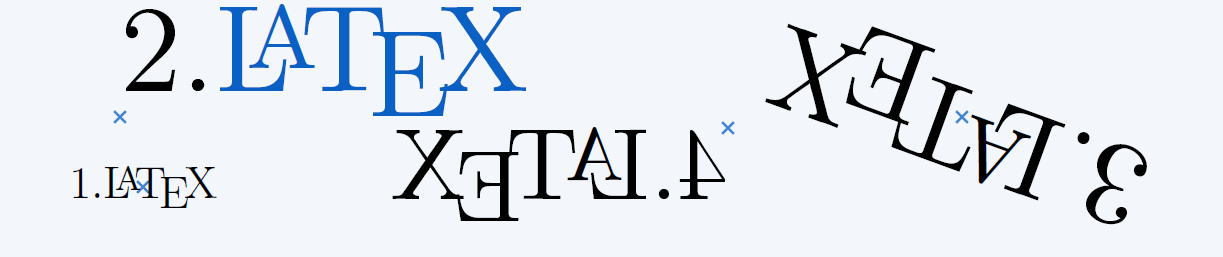
\includegraphics[width=10cm]{images/pstricks1.jpg}

\subsection{Les boîtes} \label{psboites}

Plusieurs commandes permettent d'entourer les objets. L'exemple qui suit illustre les boîtes \macro{psframebox}, \macro{psdiabox} et \macro{pscirclebox}. Les versions étoilées des boîtes permettent de les remplir\footnote{Par défaut, le remplissage est blanc uni. Ainsi, l'étoile est ici strictement équivalente à l'option \macron{fillstyle=solid}.}. L'exemple présente également la manière de saisir des options de présentation avec \paquet{pstricks} : en listant les options entre crochets sous la forme \macron{\it option = valeur} et en séparant les différentes options par des virgules. Ces options permettent, entre autres, de gérer des paramètres comme l'épaisseur de trait, le type de trait, de remplissage ou la couleur.

\begin{codedoublefig}{Boîtes}{pstricksboites}
\begin{pspicture}(10,2)
\rput(2,1){\psframebox{1.\LaTeX}}
\rput(5,0.5){\psframebox*[fillcolor=bleu6,shadow=true]{2.\LaTeX}}
\rput(5,1.5){\psdiabox[linecolor=bleu6]{3.\LaTeX}}
\rput(8,1){\pscirclebox[linestyle=dotted,linecolor=bleu6]{\Large 4.\LaTeX}}
\end{pspicture}
\end{codedoublefig}
%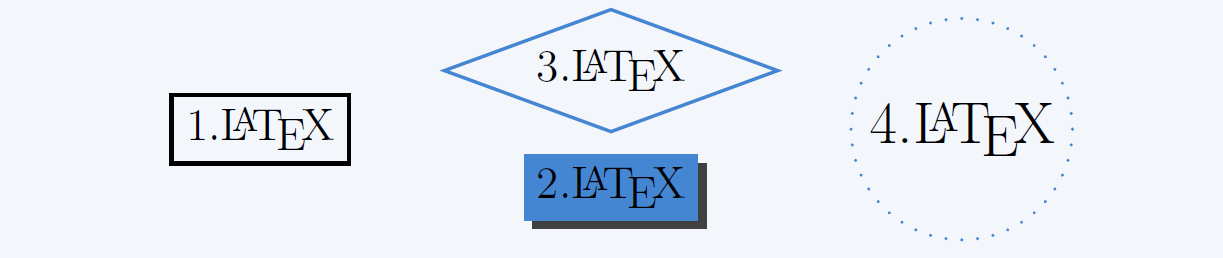
\includegraphics[width=10cm]{images/pstricks2.jpg}

\subsection{Les grilles}

Des grilles peuvent être créées aisément avec différents paramétrages. L'exemple qui suit illustre également une autre manière d'introduire la zone de tracé par l'environnement \macron{pspicture} : la donnée des coordonnées du point inférieur gauche et du point supérieur droit du cadre.

\begin{codedoublefig}{Grilles}{pstricksgrilles}
\begin{pspicture}(-0.5,-0.5)(9.5,1.5)
\psgrid(2,1.4)
\rput(3.5,0){\psgrid[griddots=10,subgriddiv=3,subgridcolor=bleu6](2,1.4)}
\rput(7,0){\psgrid[gridwidth=0.07,subgriddiv=0](2,1.4)}
\end{pspicture}
\end{codedoublefig}
%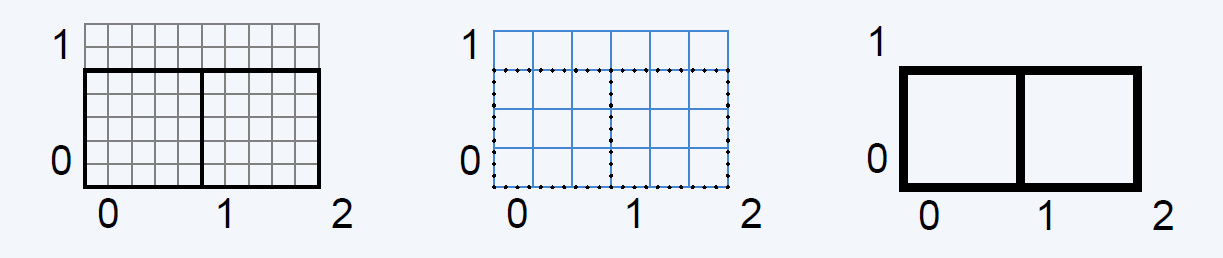
\includegraphics[width=10cm]{images/pstricks3.jpg}

\subsection{Les points et courbes}

De la même manière, \paquet{pstricks} dispose de plusieurs commandes de base pour former des traits anguleux, curvilignes. L'exemple suivant les présente sans option.

\begin{codedoublefig}{Points et courbes}{pstrickspoints}
\begin{pspicture}(-0.25,-0.5)(9.75,1.5)
\psdots(0,1)(0.5,0)(1,0.5)(1.5,0)(2,1)
\psline(2.5,1)(3,0)(3.5,0.5)(4,0)(4.5,1)
\pscurve(5,1)(5.5,0)(6,0.5)(6.5,0)(7,1)
\psccurve(7.5,1)(8,0)(8.5,0.5)(9,0)(9.5,1)
\end{pspicture}
\end{codedoublefig}
%
\includegraphics[width=10cm]{images/pstricks4.jpg}


\subsection{Les flèches et options}

Points et courbes peuvent être modifiés en donnant leur épaisseur mais aussi leur forme. Dans le cas du trait, il s'agit de la forme aux extrémités, ce qui permet en particulier d'obtenir les flèches.

\begin{codedoublefig}{Options sur points et courbes}{pstricksoptions}
\begin{pspicture}(-0.25,-0.5)(9.75,1.5)
\psdots[dotstyle=square*](0,1)(2,1)
\psdots[dotstyle=triangle,dotsize=0.2](0.5,0.2)(1,0.7)(1.5,0.2)
\psline[doubleline=true](2.5,0.7)(3,-0.3)(3.5,0.2)(4,-0.3)(4.5,0.7)
\psline[linewidth=0.1](2.5,1.3)(3,0.3)(3.5,0.8)(4,0.3)(4.5,1.3)
\pscurve[linecolor=bleu6]{|-*}(5,0.7)(5.5,-0.3)(6,0.2)(6.5,-0.3)(7,0.7)
\pscurve[arrowscale=2]{->}(5,1.3)(5.5,0.3)(6,0.8)(6.5,0.3)(7,1.3)
\psccurve*[linecolor=bleu6](7.5,1)(8,0)(8.5,0.5)(9,0)(9.5,1)
\end{pspicture}
\end{codedoublefig}
%
\includegraphics[width=10cm]{images/pstricks4.jpg}

\subsection{Vers les mathématiques}

La combinaison des éléments cités auparavant va permettre d'obtenir des graphiques mathématiques classiques : les flèches formeront les axes, les courbes la plupart des graphiques à tracer, le texte ajoutant des éléments comme les légendes des axes ou le nom des courbes. En général, il convient d'organiser les données numériques à tracer avec des logiciels permettant de concaténer des données en un format accessible à \paquet{pstricks}. En voici un exemple, obtenu avec des coordonnées mises sous forme de $(x_1,y_1)(x_2,y_2)\dots (x_n,y_n)$. 
Le code détaillé de cette figure est placé dans le fichier \macron{3oat.tex} accompagnant le fichier du cours.

\begin{figure}[H]
\centering
\begin{pspicture}(-1,-1)(11,7)
\psline[linewidth=0.01](0,2.286)(0.014,2.293)(0.028,2.34)(0.043,2.347)(0.057,2.349)(0.071,2.337)(0.085,2.322)(0.1,2.318)(0.114,2.327)(0.128,2.322)(0.142,2.297)(0.157,2.289)(0.171,2.306)(0.185,2.292)(0.199,2.206)(0.213,2.182)(0.228,2.159)(0.242,2.158)(0.256,2.157)(0.27,2.166)(0.285,2.154)(0.299,2.137)(0.313,2.124)(0.327,2.147)(0.341,2.143)(0.356,2.141)(0.37,2.136)(0.384,2.115)(0.398,2.127)(0.413,2.13)(0.427,2.122)(0.441,2.134)(0.455,2.144)(0.47,2.141)(0.484,2.139)(0.498,2.16)(0.512,2.148)(0.526,2.147)(0.541,2.139)(0.555,2.15)(0.569,2.159)(0.583,2.157)(0.598,2.144)(0.612,2.159)(0.626,2.159)(0.64,2.142)(0.654,2.146)(0.669,2.119)(0.683,2.123)(0.697,2.12)(0.711,2.117)(0.726,2.122)(0.74,2.136)(0.754,2.133)(0.768,2.13)(0.783,2.128)(0.797,2.144)(0.811,2.143)(0.825,2.135)(0.839,2.149)(0.854,2.163)(0.868,2.153)(0.882,2.144)(0.896,2.145)(0.911,2.14)(0.925,2.114)(0.939,2.119)(0.953,2.139)(0.967,2.126)(0.982,2.106)(0.996,2.102)(1.01,2.101)(1.024,2.099)(1.039,2.111)(1.053,2.073)(1.067,2.084)(1.081,2.083)(1.096,2.097)(1.11,2.08)(1.124,2.088)(1.138,2.117)(1.152,2.156)(1.167,2.15)(1.181,2.15)(1.195,2.147)(1.209,2.119)(1.224,2.103)(1.238,2.068)(1.252,2.076)(1.266,2.081)(1.28,2.08)(1.295,2.072)(1.309,2.051)(1.323,2.057)(1.337,2.005)(1.352,2.004)(1.366,2.001)(1.38,2.033)(1.394,2.042)(1.409,2.017)(1.423,1.982)(1.437,1.945)(1.451,1.919)(1.465,1.946)(1.48,1.919)(1.494,1.935)(1.508,1.912)(1.522,1.901)(1.537,1.879)(1.551,1.845)(1.565,1.899)(1.579,1.902)(1.593,1.904)(1.608,1.887)(1.622,1.914)(1.636,1.938)(1.65,1.927)(1.665,1.923)(1.679,1.926)(1.693,1.888)(1.707,1.839)(1.722,1.834)(1.736,1.803)(1.75,1.762)(1.764,1.746)(1.778,1.727)(1.793,1.705)(1.807,1.712)(1.821,1.727)(1.835,1.749)(1.85,1.696)(1.864,1.656)(1.878,1.599)(1.892,1.615)(1.907,1.588)(1.921,1.592)(1.935,1.65)(1.949,1.629)(1.963,1.604)(1.978,1.628)(1.992,1.641)(2.006,1.644)(2.02,1.613)(2.035,1.637)(2.049,1.699)(2.063,1.699)(2.077,1.691)(2.091,1.665)(2.106,1.667)(2.12,1.678)(2.134,1.726)(2.148,1.78)(2.163,1.798)(2.177,1.87)(2.191,1.906)(2.205,1.906)(2.22,1.895)(2.234,1.897)(2.248,1.943)(2.262,1.898)(2.276,1.925)(2.291,1.899)(2.305,1.878)(2.319,1.85)(2.333,1.868)(2.348,1.828)(2.362,1.844)(2.376,1.866)(2.39,1.899)(2.404,1.91)(2.419,1.861)(2.433,1.825)(2.447,1.795)(2.461,1.753)(2.476,1.755)(2.49,1.787)(2.504,1.78)(2.518,1.793)(2.533,1.779)(2.547,1.765)(2.561,1.8)(2.575,1.805)(2.589,1.818)(2.604,1.792)(2.618,1.817)(2.632,1.806)(2.646,1.786)(2.661,1.802)(2.675,1.768)(2.689,1.752)(2.703,1.735)(2.717,1.708)(2.732,1.691)(2.746,1.686)(2.76,1.667)(2.774,1.634)(2.789,1.623)(2.803,1.622)(2.817,1.606)(2.831,1.559)(2.846,1.551)(2.86,1.53)(2.874,1.525)(2.888,1.529)(2.902,1.529)(2.917,1.529)(2.931,1.45)(2.945,1.45)(2.959,1.447)(2.974,1.45)(2.988,1.504)(3.002,1.515)(3.016,1.507)(3.03,1.493)(3.045,1.46)(3.059,1.435)(3.073,1.411)(3.087,1.413)(3.102,1.392)(3.116,1.369)(3.13,1.369)(3.144,1.307)(3.159,1.28)(3.173,1.282)(3.187,1.285)(3.201,1.27)(3.215,1.223)(3.23,1.236)(3.244,1.263)(3.258,1.24)(3.272,1.249)(3.287,1.226)(3.301,1.226)(3.315,1.135)(3.329,1.082)(3.343,1.088)(3.358,1.083)(3.372,1.074)(3.386,1.071)(3.4,1.016)(3.415,0.979)(3.429,1.021)(3.443,1.038)(3.457,1.06)(3.472,1.016)(3.486,0.995)(3.5,1)(3.514,0.959)(3.528,0.921)(3.543,0.969)(3.557,1.015)(3.571,0.989)(3.585,0.972)(3.6,0.957)(3.614,0.943)(3.628,0.924)(3.642,0.895)(3.657,0.867)(3.671,0.873)(3.685,0.898)(3.699,1.023)(3.713,1.082)(3.728,1.209)(3.742,1.223)(3.756,1.29)(3.77,1.257)(3.785,1.35)(3.799,1.291)(3.813,1.277)(3.827,1.274)(3.841,1.226)(3.856,1.18)(3.87,1.107)(3.884,1.081)(3.898,1.174)(3.913,1.239)(3.927,1.25)(3.941,1.325)(3.955,1.312)(3.97,1.291)(3.984,1.245)(3.998,1.296)(4.012,1.322)(4.026,1.316)(4.041,1.276)(4.055,1.276)(4.069,1.288)(4.083,1.263)(4.098,1.238)(4.112,1.289)(4.126,1.252)(4.14,1.236)(4.154,1.25)(4.169,1.276)(4.183,1.249)(4.197,1.236)(4.211,1.219)(4.226,1.216)(4.24,1.206)(4.254,1.142)(4.268,1.112)(4.283,1.153)(4.297,1.154)(4.311,1.175)(4.325,1.171)(4.339,1.126)(4.354,1.089)(4.368,1.027)(4.382,0.993)(4.396,0.952)(4.411,0.958)(4.425,0.926)(4.439,0.906)(4.453,0.972)(4.467,1.054)(4.482,0.98)(4.496,0.978)(4.51,0.999)(4.524,0.912)(4.539,0.926)(4.553,0.87)(4.567,0.938)(4.581,0.845)(4.596,0.833)(4.61,0.784)(4.624,0.788)(4.638,0.765)(4.652,0.798)(4.667,0.87)(4.681,0.985)(4.695,0.96)(4.709,0.952)(4.724,0.928)(4.738,0.944)(4.752,0.911)(4.766,1.032)(4.78,1.056)(4.795,1.011)(4.809,1.008)(4.823,1.064)(4.837,1.106)(4.852,1.049)(4.866,1.089)(4.88,1.083)(4.894,1.091)(4.909,1.034)(4.923,0.999)(4.937,0.963)(4.951,1.047)(4.965,1.058)(4.98,1.092)(4.994,1.06)(5.008,1.092)(5.022,1.098)(5.037,1.06)(5.051,1.075)(5.065,1.023)(5.079,1.096)(5.093,1.086)(5.108,1.124)(5.122,1.185)(5.136,1.215)(5.15,1.165)(5.165,1.186)(5.179,1.168)(5.193,1.143)(5.207,1.058)(5.222,1.104)(5.236,1.096)(5.25,1.174)(5.264,1.207)(5.278,1.163)(5.293,1.17)(5.307,1.144)(5.321,1.179)(5.335,1.2)(5.35,1.185)(5.364,1.184)(5.378,1.19)(5.392,1.207)(5.407,1.186)(5.421,1.195)(5.435,1.232)(5.449,1.34)(5.463,1.367)(5.478,1.322)(5.492,1.282)(5.506,1.245)(5.52,1.263)(5.535,1.22)(5.549,1.236)(5.563,1.124)(5.577,1.139)(5.591,1.155)(5.606,1.142)(5.62,1.158)(5.634,1.121)(5.648,1.084)(5.663,1.064)(5.677,1.078)(5.691,1.053)(5.705,1.002)(5.72,1.002)(5.734,0.929)(5.748,0.943)(5.762,1.042)(5.776,1.138)(5.791,1.101)(5.805,1.11)(5.819,1.078)(5.833,1.113)(5.848,1.002)(5.862,1.047)(5.876,1.04)(5.89,1.086)(5.904,1.081)(5.919,1.096)(5.933,1.099)(5.947,1.077)(5.961,1.059)(5.976,1.075)(5.99,1.065)(6.004,1.091)(6.018,1.095)(6.033,1.073)(6.047,1.08)(6.061,1.042)(6.075,1.105)(6.089,1.068)(6.104,1.074)(6.118,1.144)(6.132,1.188)(6.146,1.178)(6.161,1.167)(6.175,1.164)(6.189,1.128)(6.203,1.096)(6.217,1.087)(6.232,1.062)(6.246,1.104)(6.26,1.084)(6.274,1.077)(6.289,1.161)(6.303,1.167)(6.317,1.157)(6.331,1.182)(6.346,1.173)(6.36,1.197)(6.374,1.168)(6.388,1.146)(6.402,1.142)(6.417,1.056)(6.431,1.071)(6.445,1.078)(6.459,1.078)(6.474,1.102)(6.488,1.069)(6.502,1.095)(6.516,1.088)(6.53,1.054)(6.545,1.063)(6.559,1.075)(6.573,1.049)(6.587,1.037)(6.602,1.036)(6.616,1.036)(6.63,1.036)(6.644,1.048)(6.659,1.045)(6.673,1.042)(6.687,1.043)(6.701,1.083)(6.715,1.065)(6.73,1.019)(6.744,1.008)(6.758,1.004)(6.772,0.933)(6.787,0.916)(6.801,0.944)(6.815,0.975)(6.829,0.978)(6.843,0.982)(6.858,0.98)(6.872,0.946)(6.886,0.939)(6.9,0.904)(6.915,0.852)(6.929,0.916)(6.943,0.928)(6.957,0.921)(6.972,1.027)(6.986,0.993) \uput[0]{0.1}(7,0.993){La première OAT}
\psline[linewidth=0.02](0,0.27)(0.014,0.288)(0.028,0.344)(0.043,0.362)(0.057,0.374)(0.071,0.372)(0.085,0.368)(0.1,0.374)(0.114,0.393)(0.128,0.398)(0.142,0.383)(0.157,0.385)(0.171,0.412)(0.185,0.408)(0.199,0.332)(0.213,0.318)(0.228,0.306)(0.242,0.315)(0.256,0.324)(0.27,0.343)(0.285,0.341)(0.299,0.334)(0.313,0.331)(0.327,0.365)(0.341,0.371)(0.356,0.379)(0.37,0.384)(0.384,0.373)(0.398,0.395)(0.413,0.408)(0.427,0.41)(0.441,0.432)(0.455,0.453)(0.47,0.46)(0.484,0.468)(0.498,0.499)(0.512,0.497)(0.526,0.506)(0.541,0.508)(0.555,0.53)(0.569,0.549)(0.583,0.557)(0.598,0.554)(0.612,0.579)(0.626,0.589)(0.64,0.582)(0.654,0.597)(0.669,0.579)(0.683,0.594)(0.697,0.601)(0.711,0.608)(0.726,0.623)(0.74,0.647)(0.754,0.654)(0.768,0.661)(0.783,0.669)(0.797,0.696)(0.811,0.705)(0.825,0.707)(0.839,0.731)(0.854,0.756)(0.868,0.756)(0.882,0.757)(0.896,0.768)(0.911,0.773)(0.925,0.757)(0.939,0.772)(0.953,0.802)(0.967,0.799)(0.982,0.789)(0.996,0.795)(1.01,0.804)(1.024,0.812)(1.039,0.835)(1.053,0.807)(1.067,0.828)(1.081,0.838)(1.096,0.861)(1.11,0.855)(1.124,0.873)(1.138,0.912)(1.152,0.961)(1.167,0.965)(1.181,0.975)(1.195,0.982)(1.209,0.964)(1.224,0.958)(1.238,0.934)(1.252,0.952)(1.266,0.967)(1.28,0.976)(1.295,0.978)(1.309,0.967)(1.323,0.983)(1.337,0.942)(1.352,0.951)(1.366,0.958)(1.38,1)(1.394,1.019)(1.409,1.004)(1.423,0.979)(1.437,0.952)(1.451,0.937)(1.465,0.973)(1.48,0.957)(1.494,0.982)(1.508,0.97)(1.522,0.969)(1.537,0.957)(1.551,0.934)(1.565,0.998)(1.579,1.011)(1.593,1.023)(1.608,1.016)(1.622,1.053)(1.636,1.087)(1.65,1.087)(1.665,1.093)(1.679,1.106)(1.693,1.078)(1.707,1.039)(1.722,1.044)(1.736,1.023)(1.75,0.993)(1.764,0.986)(1.778,0.977)(1.793,0.965)(1.807,0.982)(1.821,1.008)(1.835,1.04)(1.85,0.998)(1.864,0.967)(1.878,0.921)(1.892,0.947)(1.907,0.93)(1.921,0.944)(1.935,1.012)(1.949,1.001)(1.963,0.986)(1.978,1.02)(1.992,1.043)(2.006,1.056)(2.02,1.036)(2.035,1.07)(2.049,1.141)(2.063,1.152)(2.077,1.155)(2.091,1.138)(2.106,1.151)(2.12,1.172)(2.134,1.23)(2.148,1.293)(2.163,1.322)(2.177,1.404)(2.191,1.45)(2.205,1.46)(2.22,1.459)(2.234,1.472)(2.248,1.527)(2.262,1.493)(2.276,1.53)(2.291,1.514)(2.305,1.503)(2.319,1.486)(2.333,1.513)(2.348,1.484)(2.362,1.51)(2.376,1.542)(2.39,1.585)(2.404,1.606)(2.419,1.567)(2.433,1.542)(2.447,1.521)(2.461,1.49)(2.476,1.502)(2.49,1.544)(2.504,1.547)(2.518,1.57)(2.533,1.566)(2.547,1.563)(2.561,1.607)(2.575,1.623)(2.589,1.646)(2.604,1.63)(2.618,1.665)(2.632,1.664)(2.646,1.654)(2.661,1.68)(2.675,1.657)(2.689,1.651)(2.703,1.644)(2.717,1.627)(2.732,1.621)(2.746,1.626)(2.76,1.616)(2.774,1.593)(2.789,1.592)(2.803,1.601)(2.817,1.596)(2.831,1.559)(2.846,1.561)(2.86,1.551)(2.874,1.556)(2.888,1.57)(2.902,1.58)(2.917,1.59)(2.931,1.521)(2.945,1.531)(2.959,1.538)(2.974,1.552)(2.988,1.615)(3.002,1.637)(3.016,1.639)(3.03,1.635)(3.045,1.612)(3.059,1.597)(3.073,1.583)(3.087,1.595)(3.102,1.584)(3.116,1.572)(3.13,1.582)(3.144,1.529)(3.159,1.513)(3.173,1.525)(3.187,1.538)(3.201,1.533)(3.215,1.497)(3.23,1.519)(3.244,1.557)(3.258,1.544)(3.272,1.563)(3.287,1.55)(3.301,1.56)(3.315,1.48)(3.329,1.436)(3.343,1.452)(3.358,1.457)(3.372,1.458)(3.386,1.466)(3.4,1.421)(3.415,1.395)(3.429,1.446)(3.443,1.474)(3.457,1.506)(3.472,1.472)(3.486,1.46)(3.5,1.476)(3.514,1.445)(3.528,1.417)(3.543,1.476)(3.557,1.531)(3.571,1.515)(3.585,1.509)(3.6,1.504)(3.614,1.5)(3.628,1.491)(3.642,1.473)(3.657,1.454)(3.671,1.471)(3.685,1.506)(3.699,1.641)(3.713,1.71)(3.728,1.847)(3.742,1.872)(3.756,1.949)(3.77,1.925)(3.785,2.029)(3.799,1.98)(3.813,1.976)(3.827,1.983)(3.841,1.945)(3.856,1.909)(3.87,1.846)(3.884,1.83)(3.898,1.933)(3.913,2.008)(3.927,2.03)(3.941,2.115)(3.955,2.112)(3.97,2.102)(3.984,2.065)(3.998,2.127)(4.012,2.162)(4.026,2.166)(4.041,2.137)(4.055,2.147)(4.069,2.169)(4.083,2.154)(4.098,2.139)(4.112,2.201)(4.126,2.174)(4.14,2.167)(4.154,2.192)(4.169,2.228)(4.183,2.211)(4.197,2.208)(4.211,2.202)(4.226,2.209)(4.24,2.209)(4.254,2.155)(4.268,2.135)(4.283,2.186)(4.297,2.197)(4.311,2.228)(4.325,2.234)(4.339,2.2)(4.354,2.173)(4.368,2.121)(4.382,2.097)(4.396,2.066)(4.411,2.082)(4.425,2.06)(4.439,2.051)(4.453,2.127)(4.467,2.219)(4.482,2.155)(4.496,2.163)(4.51,2.194)(4.524,2.117)(4.539,2.141)(4.553,2.096)(4.567,2.174)(4.581,2.09)(4.596,2.088)(4.61,2.05)(4.624,2.064)(4.638,2.051)(4.652,2.095)(4.667,2.177)(4.681,2.302)(4.695,2.287)(4.709,2.289)(4.724,2.275)(4.738,2.301)(4.752,2.278)(4.766,2.41)(4.78,2.444)(4.795,2.409)(4.809,2.416)(4.823,2.482)(4.837,2.534)(4.852,2.488)(4.866,2.537)(4.88,2.541)(4.894,2.559)(4.909,2.513)(4.923,2.488)(4.937,2.462)(4.951,2.556)(4.965,2.578)(4.98,2.621)(4.994,2.6)(5.008,2.641)(5.022,2.658)(5.037,2.63)(5.051,2.655)(5.065,2.613)(5.079,2.696)(5.093,2.696)(5.108,2.745)(5.122,2.816)(5.136,2.856)(5.15,2.816)(5.165,2.847)(5.179,2.839)(5.193,2.825)(5.207,2.75)(5.222,2.806)(5.236,2.808)(5.25,2.896)(5.264,2.939)(5.278,2.905)(5.293,2.922)(5.307,2.907)(5.321,2.951)(5.335,2.983)(5.35,2.978)(5.364,2.987)(5.378,3.003)(5.392,3.03)(5.407,3.019)(5.421,3.038)(5.435,3.085)(5.449,3.204)(5.463,3.241)(5.478,3.206)(5.492,3.176)(5.506,3.149)(5.52,3.177)(5.535,3.145)(5.549,3.17)(5.563,3.069)(5.577,3.094)(5.591,3.12)(5.606,3.117)(5.62,3.143)(5.634,3.116)(5.648,3.089)(5.663,3.08)(5.677,3.103)(5.691,3.089)(5.705,3.048)(5.72,3.058)(5.734,2.995)(5.748,3.019)(5.762,3.129)(5.776,3.235)(5.791,3.208)(5.805,3.227)(5.819,3.205)(5.833,3.25)(5.848,3.149)(5.862,3.205)(5.876,3.208)(5.89,3.263)(5.904,3.268)(5.919,3.294)(5.933,3.307)(5.947,3.295)(5.961,3.288)(5.976,3.313)(5.99,3.314)(6.004,3.349)(6.018,3.364)(6.033,3.351)(6.047,3.369)(6.061,3.341)(6.075,3.414)(6.089,3.387)(6.104,3.403)(6.118,3.484)(6.132,3.538)(6.146,3.538)(6.161,3.537)(6.175,3.544)(6.189,3.519)(6.203,3.496)(6.217,3.497)(6.232,3.483)(6.246,3.535)(6.26,3.525)(6.274,3.528)(6.289,3.622)(6.303,3.638)(6.317,3.638)(6.331,3.674)(6.346,3.675)(6.36,3.709)(6.374,3.69)(6.388,3.678)(6.402,3.685)(6.417,3.609)(6.431,3.633)(6.445,3.65)(6.459,3.66)(6.474,3.695)(6.488,3.672)(6.502,3.708)(6.516,3.711)(6.53,3.688)(6.545,3.707)(6.559,3.728)(6.573,3.713)(6.587,3.711)(6.602,3.72)(6.616,3.73)(6.63,3.74)(6.644,3.763)(6.659,3.77)(6.673,3.777)(6.687,3.788)(6.701,3.838)(6.715,3.831)(6.73,3.794)(6.744,3.793)(6.758,3.799)(6.772,3.738)(6.787,3.731)(6.801,3.77)(6.815,3.811)(6.829,3.824)(6.843,3.839)(6.858,3.847)(6.872,3.822)(6.886,3.825)(6.9,3.801)(6.915,3.759)(6.929,3.833)(6.943,3.855)(6.957,3.858)(6.972,3.974)(6.986,3.95) \uput[0]{0.1}(7,3.95){La deuxième OAT}
\psline[linewidth=0.03](0,0.591)(0.014,0.64)(0.028,0.654)(0.043,0.735)(0.057,0.769)(0.071,0.852)(0.085,0.921)(0.1,0.99)(0.114,1.058)(0.128,1.154)(0.142,1.207)(0.157,1.235)(0.171,1.309)(0.185,1.34)(0.199,1.391)(0.213,1.407)(0.228,1.436)(0.242,1.511)(0.256,1.55)(0.27,1.576)(0.285,1.666)(0.299,1.725)(0.313,1.783)(0.327,1.792)(0.341,1.812)(0.356,1.829)(0.37,1.878)(0.384,1.883)(0.398,1.947)(0.413,2.003)(0.427,2.024)(0.441,2.106)(0.455,2.175)(0.47,2.19)(0.484,2.288)(0.498,2.308)(0.512,2.317)(0.526,2.405)(0.541,2.477)(0.555,2.524)(0.569,2.575)(0.583,2.583)(0.598,2.58)(0.612,2.605)(0.626,2.615)(0.64,2.608)(0.654,2.622)(0.669,2.605)(0.683,2.619)(0.697,2.626)(0.711,2.633)(0.726,2.649)(0.74,2.673)(0.754,2.68)(0.768,2.687)(0.783,2.695)(0.797,2.721)(0.811,2.731)(0.825,2.733)(0.839,2.757)(0.854,2.781)(0.868,2.781)(0.882,2.782)(0.896,2.793)(0.911,2.798)(0.925,2.782)(0.939,2.797)(0.953,2.828)(0.967,2.825)(0.982,2.815)(0.996,2.821)(1.01,2.83)(1.024,2.838)(1.039,2.86)(1.053,2.833)(1.067,2.854)(1.081,2.863)(1.096,2.887)(1.11,2.88)(1.124,2.899)(1.138,2.937)(1.152,2.987)(1.167,2.991)(1.181,3.001)(1.195,3.008)(1.209,2.99)(1.224,2.984)(1.238,2.959)(1.252,2.978)(1.266,2.993)(1.28,3.002)(1.295,3.004)(1.309,2.993)(1.323,3.009)(1.337,2.968)(1.352,2.977)(1.366,2.984)(1.38,3.025)(1.394,3.045)(1.409,3.029)(1.423,3.005)(1.437,2.978)(1.451,2.963)(1.465,2.999)(1.48,2.983)(1.494,3.008)(1.508,2.996)(1.522,2.995)(1.537,2.983)(1.551,2.959)(1.565,3.023)(1.579,3.036)(1.593,3.049)(1.608,3.042)(1.622,3.079)(1.636,3.112)(1.65,3.112)(1.665,3.119)(1.679,3.132)(1.693,3.103)(1.707,3.065)(1.722,3.07)(1.736,3.049)(1.75,3.018)(1.764,3.012)(1.778,3.003)(1.793,2.991)(1.807,3.008)(1.821,3.033)(1.835,3.066)(1.85,3.023)(1.864,2.993)(1.878,2.946)(1.892,2.973)(1.907,2.955)(1.921,2.97)(1.935,3.037)(1.949,3.026)(1.963,3.012)(1.978,3.046)(1.992,3.069)(2.006,3.082)(2.02,3.062)(2.035,3.095)(2.049,3.167)(2.063,3.177)(2.077,3.18)(2.091,3.164)(2.106,3.176)(2.12,3.198)(2.134,3.255)(2.148,3.319)(2.163,3.347)(2.177,3.429)(2.191,3.476)(2.205,3.486)(2.22,3.485)(2.234,3.497)(2.248,3.553)(2.262,3.519)(2.276,3.556)(2.291,3.54)(2.305,3.529)(2.319,3.511)(2.333,3.539)(2.348,3.509)(2.362,3.536)(2.376,3.567)(2.39,3.611)(2.404,3.632)(2.419,3.593)(2.433,3.567)(2.447,3.547)(2.461,3.516)(2.476,3.528)(2.49,3.569)(2.504,3.572)(2.518,3.596)(2.533,3.591)(2.547,3.588)(2.561,3.633)(2.575,3.648)(2.589,3.672)(2.604,3.655)(2.618,3.691)(2.632,3.69)(2.646,3.68)(2.661,3.706)(2.675,3.683)(2.689,3.677)(2.703,3.669)(2.717,3.652)(2.732,3.646)(2.746,3.651)(2.76,3.642)(2.774,3.619)(2.789,3.618)(2.803,3.627)(2.817,3.622)(2.831,3.584)(2.846,3.586)(2.86,3.576)(2.874,3.581)(2.888,3.596)(2.902,3.606)(2.917,3.616)(2.931,3.547)(2.945,3.557)(2.959,3.564)(2.974,3.577)(2.988,3.641)(3.002,3.662)(3.016,3.664)(3.03,3.66)(3.045,3.638)(3.059,3.623)(3.073,3.609)(3.087,3.621)(3.102,3.61)(3.116,3.598)(3.13,3.608)(3.144,3.555)(3.159,3.539)(3.173,3.551)(3.187,3.564)(3.201,3.559)(3.215,3.523)(3.23,3.545)(3.244,3.582)(3.258,3.569)(3.272,3.588)(3.287,3.575)(3.301,3.585)(3.315,3.505)(3.329,3.462)(3.343,3.478)(3.358,3.483)(3.372,3.484)(3.386,3.491)(3.4,3.447)(3.415,3.42)(3.429,3.472)(3.443,3.499)(3.457,3.532)(3.472,3.497)(3.486,3.486)(3.5,3.501)(3.514,3.471)(3.528,3.443)(3.543,3.501)(3.557,3.557)(3.571,3.541)(3.585,3.535)(3.6,3.53)(3.614,3.526)(3.628,3.517)(3.642,3.498)(3.657,3.48)(3.671,3.496)(3.685,3.532)(3.699,3.666)(3.713,3.735)(3.728,3.873)(3.742,3.897)(3.756,3.974)(3.77,3.951)(3.785,4.054)(3.799,4.006)(3.813,4.002)(3.827,4.009)(3.841,3.97)(3.856,3.935)(3.87,3.872)(3.884,3.856)(3.898,3.959)(3.913,4.034)(3.927,4.055)(3.941,4.14)(3.955,4.137)(3.97,4.127)(3.984,4.091)(3.998,4.153)(4.012,4.188)(4.026,4.192)(4.041,4.163)(4.055,4.173)(4.069,4.195)(4.083,4.18)(4.098,4.165)(4.112,4.227)(4.126,4.199)(4.14,4.193)(4.154,4.217)(4.169,4.254)(4.183,4.237)(4.197,4.234)(4.211,4.228)(4.226,4.235)(4.24,4.235)(4.254,4.181)(4.268,4.161)(4.283,4.211)(4.297,4.222)(4.311,4.254)(4.325,4.26)(4.339,4.226)(4.354,4.198)(4.368,4.147)(4.382,4.122)(4.396,4.092)(4.411,4.108)(4.425,4.086)(4.439,4.077)(4.453,4.153)(4.467,4.245)(4.482,4.181)(4.496,4.189)(4.51,4.219)(4.524,4.142)(4.539,4.167)(4.553,4.121)(4.567,4.199)(4.581,4.116)(4.596,4.114)(4.61,4.076)(4.624,4.09)(4.638,4.077)(4.652,4.12)(4.667,4.202)(4.681,4.328)(4.695,4.313)(4.709,4.315)(4.724,4.3)(4.738,4.327)(4.752,4.304)(4.766,4.435)(4.78,4.47)(4.795,4.434)(4.809,4.441)(4.823,4.508)(4.837,4.56)(4.852,4.513)(4.866,4.563)(4.88,4.567)(4.894,4.585)(4.909,4.538)(4.923,4.513)(4.937,4.488)(4.951,4.582)(4.965,4.603)(4.98,4.647)(4.994,4.626)(5.008,4.667)(5.022,4.683)(5.037,4.656)(5.051,4.68)(5.065,4.639)(5.079,4.722)(5.093,4.722)(5.108,4.77)(5.122,4.841)(5.136,4.882)(5.15,4.841)(5.165,4.873)(5.179,4.865)(5.193,4.85)(5.207,4.775)(5.222,4.831)(5.236,4.833)(5.25,4.921)(5.264,4.965)(5.278,4.93)(5.293,4.948)(5.307,4.932)(5.321,4.977)(5.335,5.008)(5.35,5.003)(5.364,5.012)(5.378,5.029)(5.392,5.056)(5.407,5.045)(5.421,5.064)(5.435,5.111)(5.449,5.229)(5.463,5.267)(5.478,5.231)(5.492,5.202)(5.506,5.175)(5.52,5.203)(5.535,5.17)(5.549,5.196)(5.563,5.095)(5.577,5.12)(5.591,5.145)(5.606,5.143)(5.62,5.168)(5.634,5.142)(5.648,5.115)(5.663,5.106)(5.677,5.129)(5.691,5.115)(5.705,5.073)(5.72,5.083)(5.734,5.021)(5.748,5.045)(5.762,5.154)(5.776,5.261)(5.791,5.233)(5.805,5.253)(5.819,5.23)(5.833,5.276)(5.848,5.175)(5.862,5.23)(5.876,5.233)(5.89,5.289)(5.904,5.294)(5.919,5.319)(5.933,5.333)(5.947,5.32)(5.961,5.313)(5.976,5.339)(5.99,5.34)(6.004,5.375)(6.018,5.389)(6.033,5.377)(6.047,5.394)(6.061,5.367)(6.075,5.44)(6.089,5.413)(6.104,5.429)(6.118,5.51)(6.132,5.563)(6.146,5.563)(6.161,5.562)(6.175,5.57)(6.189,5.544)(6.203,5.522)(6.217,5.523)(6.232,5.509)(6.246,5.56)(6.26,5.55)(6.274,5.553)(6.289,5.648)(6.303,5.664)(6.317,5.664)(6.331,5.699)(6.346,5.7)(6.36,5.735)(6.374,5.715)(6.388,5.703)(6.402,5.71)(6.417,5.634)(6.431,5.659)(6.445,5.676)(6.459,5.686)(6.474,5.72)(6.488,5.697)(6.502,5.734)(6.516,5.737)(6.53,5.713)(6.545,5.733)(6.559,5.754)(6.573,5.739)(6.587,5.737)(6.602,5.746)(6.616,5.756)(6.63,5.766)(6.644,5.788)(6.659,5.795)(6.673,5.802)(6.687,5.814)(6.701,5.863)(6.715,5.856)(6.73,5.82)(6.744,5.819)(6.758,5.825)(6.772,5.764)(6.787,5.757)(6.801,5.795)(6.815,5.837)(6.829,5.85)(6.843,5.864)(6.858,5.872)(6.872,5.848)(6.886,5.851)(6.9,5.827)(6.915,5.784)(6.929,5.858)(6.943,5.88)(6.957,5.884)(6.972,6)(6.986,5.976) \uput[0]{0.1}(7,5.976){La dernière OAT}
\psline{->}(-0.1,0)(7.2,0)
\uput[0](7.4,0){Date}
\psline{->}(0,-0.1)(0,6.2)
\rput(0,6.5){Taux}
\psline(-0.1,1.013)(0.1,1.013) \uput[180]{0}(-0.1,1.013){2\%}\psline(-0.1,2.026)(0.1,2.026) \uput[180]{0}(-0.1,2.026){3\%}\psline(-0.1,3.038)(0.1,3.038) \uput[180]{0}(-0.1,3.038){4\%}\psline(-0.1,4.051)(0.1,4.051) \uput[180]{0}(-0.1,4.051){5\%}\psline(-0.1,5.064)(0.1,5.064) \uput[180]{0}(-0.1,5.064){6\%}

\psline(0,-0.1)(0,0.1) \uput[270]{45}(0,-0.1){3/99}\psline(0.868,-0.1)(0.868,0.1) \uput[270]{45}(0.868,-0.1){5/99}\psline(1.736,-0.1)(1.736,0.1) \uput[270]{45}(1.736,-0.1){7/99}\psline(2.618,-0.1)(2.618,0.1) \uput[270]{45}(2.618,-0.1){9/99}\psline(3.486,-0.1)(3.486,0.1) \uput[270]{45}(3.486,-0.1){11/99}\psline(4.354,-0.1)(4.354,0.1) \uput[270]{45}(4.354,-0.1){1/00}\psline(5.207,-0.1)(5.207,0.1) \uput[270]{45}(5.207,-0.1){3/00}\psline(6.075,-0.1)(6.075,0.1) \uput[270]{45}(6.075,-0.1){5/00}\psline(6.986,-0.1)(6.986,0.1) \uput[270]{45}(6.986,-0.1){7/00}

\end{pspicture}
\caption{Quelques OAT}\label{3oat}
\end{figure}

%%%% Ajout YT récent %%%% 
\subsection{Le tracé de fonction mathématique}

Le paquet \paquet{pst-plot}, un des paquets spécialisés se basant sur \paquet{pstricks}, contient quelques  commandes de traçage non négligeables. La plus simple,\macro{psaxes}, trace des axes à nos figures.

\subsubsection{La notation des fonctions}

L'appel du paquet \paquet{pst-plot} permet d'utiliser en particulier les notations mathématiques usuelles avec l'option \macron{algebraic=true} à placer parmi les options des commandes \macro{psplot} et \macro{parametricplot}, comme l'illustrent les exemples qui suivent. Sans cette option, les notations doivent se faire selon une notation polonaise inversée\footnote{Cette notation n'utilise pas la notion de parenthèses. Pour cela, les opérateurs se placent après les opérandes sur lesquels ils s'appliquent. Plus exactement, les termes se lisent successivement : si un terme est un opérande, il est stocké. Si c'est un opérateur, il s'applique aux derniers opérandes stockés.}.

La notation\footnote{Voir par exemple \liensimple{http://ww2.ac-poitiers.fr/math/spip.php?article134&debut_page=1}.} travaille en radian et non en degré. Dans le cas d'une  commande paramétrique, la variable muette est \macron{t} et il faut indiquer une séparation avec un \macron{|} entre les deux fonctions paramétriques du \macro{parametricplot}.

\subsubsection{Une fonction classique}

Voici donc l'exemple de la fonction $sin (2x)$.

\codefigure{
\macro{begin}\{pspicture\}(-1,-1.25)(7,1.25) \\
\macro{psplot}[plotstyle=curve,plotpoints=199,linecolor=bleu8,algebraic=true]\{0\}\{6\}\{sin(2*x)\} \\
\macro{psaxes}(0,0)(-0.5,-1.25)(6.25,1.25) \\
\macro{end}\{pspicture\}
}{
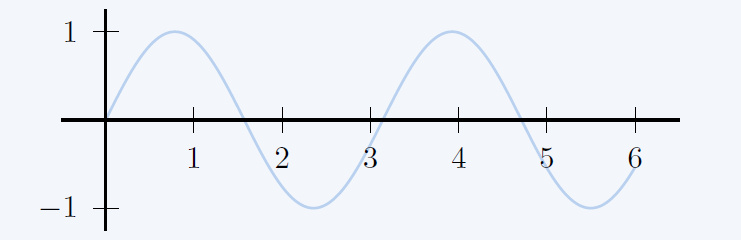
\includegraphics[width=8cm]{images/sinus.jpg}
%\begin{pspicture}(-1,-1.25)(7,1.25)
%\psplot[plotstyle=curve,plotpoints=199,linecolor=bleu8,algebraic=true]{0}{6}{sin(2*x)}
%\psaxes(0,0)(-0.5,-1.25)(6.5,1.25)
%\end{pspicture}
}{Une sinusoïde}

L'option \macron{plotpoints} indique de plus le nombre de points à calculer pour tracer la courbe. Par ailleurs, l'option \macron{plotstyle} permet de préciser avec la valeur \macron{curve} que le tracé de la fonction se fait par courbe, autrement dit qu'il est lissé (il pourrait se faire par ligne avec la valeur \macron{line} ou par de simples points avec \macron{dots}). 

\subsubsection{Une fonction paramétrique}

Pour des fonctions paramétrées, il faut mettre à la suite les fonctions de chaque coordonnées l'une après l'autre, \LaTeX\ repérant les deux fonctions du fait de la notation polonaise inversée. Voici l'exemple d'une rosace avec \macro{parametricplot} :

$$
\left\{
\begin{array}{lcr}
x(t)&=& 2 \sin 4t \cos 5t \\
y(t)&=& 2 \cos 4t \cos 5t 
\end{array}
\right.
$$

\codefigure{
\macro{begin}\{pspicture\}(-2.15,-2.15)(2.15,2.15)  \\
\macro{parametricplot}[plotstyle=curve,plotpoints=199,linecolor=bleu8,algebraic=true]\{0\}\{6.3\}\\\{2*(sin(4*t))*(cos(5*t))|2*(cos(4*t))*(cos(5*t))\} \\
\macro{psaxes}(0,0)(-2.1,-2.1)(2.1,2.1) \\
\macro{end}\{pspicture\}
}{
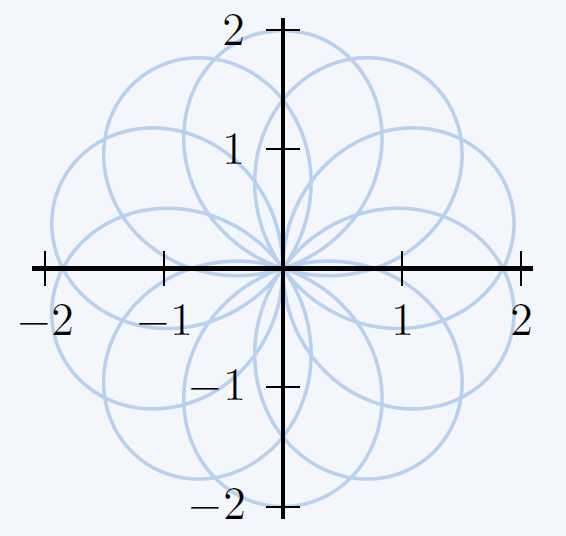
\includegraphics[width=4.3cm]{images/rosace.jpg}
%\begin{pspicture}(-2.15,-2.15)(2.15,2.15)
%\parametricplot[plotstyle=curve,plotpoints=199,linecolor=bleu8,algebraic=true]{0}{6.3}{2*(sin(4*t))*(cos(5*t))|2*(cos(4*t))*(cos(5*t))}
%\psaxes(0,0)(-2.1,-2.1)(2.1,2.1)
%\end{pspicture}
}{Une rosace}


\subsection{Exemples capillotractés} 

\subsubsection{Un histogramme}

Les  commandes de \paquet{pstricks} peuvent être combinées encore plus fortement, jusqu'à définir un ensemble de  commandes dédiées à des traitements particuliers. Il faut ici combiner utilisation de \paquet{pstricks} et programmation.

Voici, pour illustrer ce point, un histogramme obtenu avec un paquet inconnu car fait maison : \paquet{histogra}\footnote{Ce paquet est très peu documenté et encore moins développé pour servir partout... il n'a servi que pour réaliser quelques figures dans un document bien précis.}.

%\sethisto{inter=0,large=0.25,hcol1=bleu5}

\begin{figure}[H]
\begin{center}
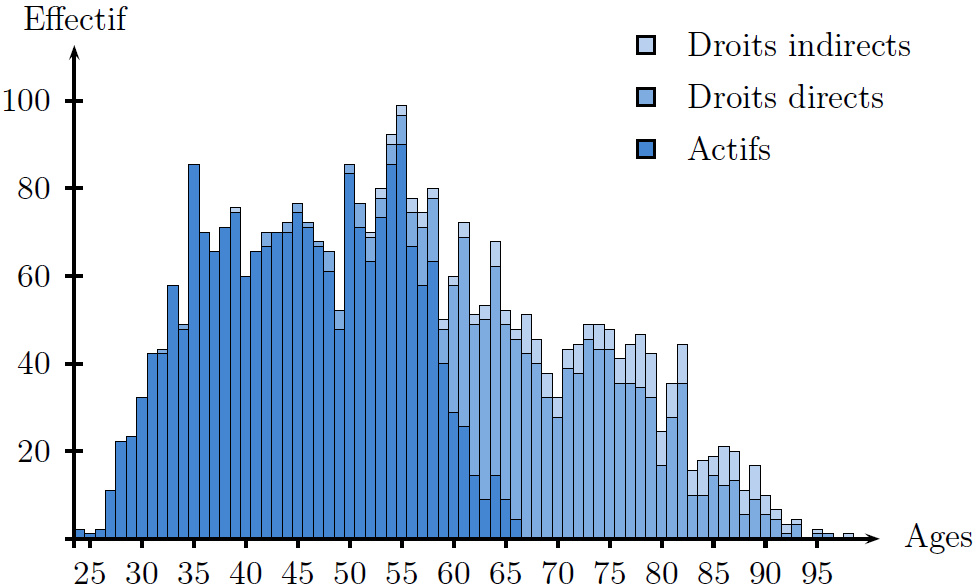
\includegraphics[width=11cm]{images/histogra.jpg}
%\begin{pspicture}(-0.5,-0.5)(10.5,6.5)
%
%\psset{dimen=middle,fillstyle=solid}
%\psframe[fillcolor=bleu8](6.5,5.6)(6.7,5.8) \uput[0]{0}(6.9,5.7){Droits indirects}
%\psframe[fillcolor=bleu7](6.5,5)(6.7,5.2)   \uput[0]{0}(6.9,5.1){Droits directs}
%\psframe[fillcolor=bleu6](6.5,4.4)(6.7,4.6) \uput[0]{0}(6.9,4.5){Actifs}
%
%\essai[inter=0,large=0.12,hcol1=bleu6,hcol2=bleu7,hcol3=bleu8,epais=0.3pt]{(0.2,0,0)(0.1,0,0)(0.2,0,0)(1,0,0)(2,0,0)(2.1,0,0)(2.9,0,0)(3.8,0,0)(3.8,0.1,0)(5.2,0,0)(4.3,0.1,0)(7.7,0,0)(6.3,0,0)(5.9,0,0)(6.4,0,0)(6.7,0,0.1)(5.4,0,0)(5.9,0,0)(6,0.3,0)(6.3,0,0)(6.3,0.2,0)(6.7,0.2,0)(6.4,0.1,0)(6,0.1,0)(5.5,0.4,0)(4.3,0.4,0)(7.5,0.2,0)(6.4,0.5,0)(5.7,0.5,0.1)(6.6,0.4,0.2)(7.7,0.4,0.2)(8.1,0.6,0.2)(6,0.7,0.3)(5.2,1.2,0.3)(5.7,1.3,0.2)(3.6,0.7,0.2)(2.6,2.6,0.2)(2.3,3.9,0.3)(1.3,3.1,0.2)(0.8,3.7,0.3)(1.3,4.3,0.5)(0.8,3.6,0.3)(0.4,3.7,0.2)(0,3.8,0.8)(0,3.6,0.5)(0,2.9,0.5)(0,2.5,0.4)(0,3.5,0.4)(0,3.4,0.6)(0,4.1,0.3)(0,3.9,0.5)(0,3.9,0.4)(0,3.2,0.5)(0,3.2,0.8)(0,3.1,1.1)(0,2.9,0.9)(0,1.5,0.7)(0,2.5,0.7)(0,3.2,0.8)(0,0.9,0.5)(0,0.9,0.7)(0,1.3,0.4)(0,1.1,0.8)(0,1.2,0.6)(0,0.5,0.5)(0,0.8,0.7)(0,0.5,0.4)(0,0.4,0.2)(0,0.1,0.2)(0,0.3,0.1)(0,0,0)(0,0.1,0.1)(0,0.1,0)(0,0,0)(0,0,0.1)(0,0,0)}
%
%\psset{linewidth=1pt}
%\axex(9.3,Ages)
%\axey(5.7,Effectif)
%
%\end{pspicture}
\end{center}
\caption{Pyramide des effectifs}
\end{figure}

%\end{document}

\subsubsection{Une famille de courbes} \label{famillecourbe}

Ce qui suit utilise un mélange de commandes tirées des paquets \paquet{pstricks} et \paquet{multido}. Est tracé ici une famille de figures paramétrées définie par le système suivant :

$$
\left\{
\begin{array}{lcr}
x(t)&=& 0,9 \cos \alpha t \\
y(t)&=& 0,9 \sin \beta t  
\end{array}  \quad \textrm{avec } (\alpha,\beta) \in [1..5]\times[1..6]
\right.
$$

Pour faire ce tracé, une commande un peu plus générale est définie. Dans celle-ci, \paquet{multido} permet de faire deux boucles imbriquées (une sur $\alpha$, l'autre sur $\beta$) et \paquet{pst-plot} permet de tracer la figure voulue.

\begin{codesimple}{Construction d'une famille de courbes}{codfamillecourbe}
\newcommand{\figu}[1]{
\begin{figure}[H]
\begin{center}
\fbox{
\begin{pspicture}(12.3,15.2)
  \multido{\Na=1.1+2.5,\Ia=1+1}{5}{
    \multido{\Nb=13.9+-2.5,\Ib=1+1}{6}{
      \rput{0}(\Na,\Nb){
        \parametricplot[plotstyle=curve,plotpoints=199,linecolor=bleu6,
        algebraic=true]{0}{6.2832}{#1}
        \rput{0}(0,-1.2){\textsf{\footnotesize (\Ia,\Ib)}}}
}}
\end{pspicture}}
\caption{Exemples de fonctions paramétriques}
\end{center}
\end{figure}}
\end{codesimple}


Ainsi, l'utilisation de la  commande s'est limitée à l'appel qui suit. Cependant, en terme de présentation, cette  commande devrait disposer de plus de paramètres que les formules. Sans cela, la légende, le nombre de figures tracées et leur précision ne peuvent être modifiés aisément.

\begin{codesimple}{Appel de la  commande pour les courbes}{appelcourbes}
\figu{0.9*cos(t*\Ia)|0.9*sin(t*\Ib)}
\end{codesimple}


% Ci-dessous la fonction générale
\newcommand{\figu}[1]{
\begin{figure}[H]
\begin{center}
\fbox{
\begin{pspicture}(12.3,15.2)
  \multido{\Na=1.1+2.5,\Ia=1+1}{5}{
    \multido{\Nb=13.9+-2.5,\Ib=1+1}{6}{
      \rput{0}(\Na,\Nb){
        \parametricplot[plotstyle=curve,plotpoints=199,linecolor=bleu6,algebraic=true]{0}{6.2832}{#1}
        \rput{0}(0,-1.2){\textsf{\footnotesize (\Ia,\Ib)}}}
}}
\end{pspicture}}
$$
\left\{
\begin{array}{lcr}
x(t)&=& 0,9 \cos \alpha t \\
y(t)&=& 0,9 \sin \beta t  
\end{array}  \quad \textrm{avec } (\alpha,\beta) \in [1..5]\times[1..6]
\right.
$$
\caption{Exemples de fonctions paramétriques}
\end{center}
\end{figure}
}

%\figu{0.9*cos(t*\Ia)|0.9*sin(t*\Ib)} 

\begin{figure}[H]
\begin{center}
\fbox{%
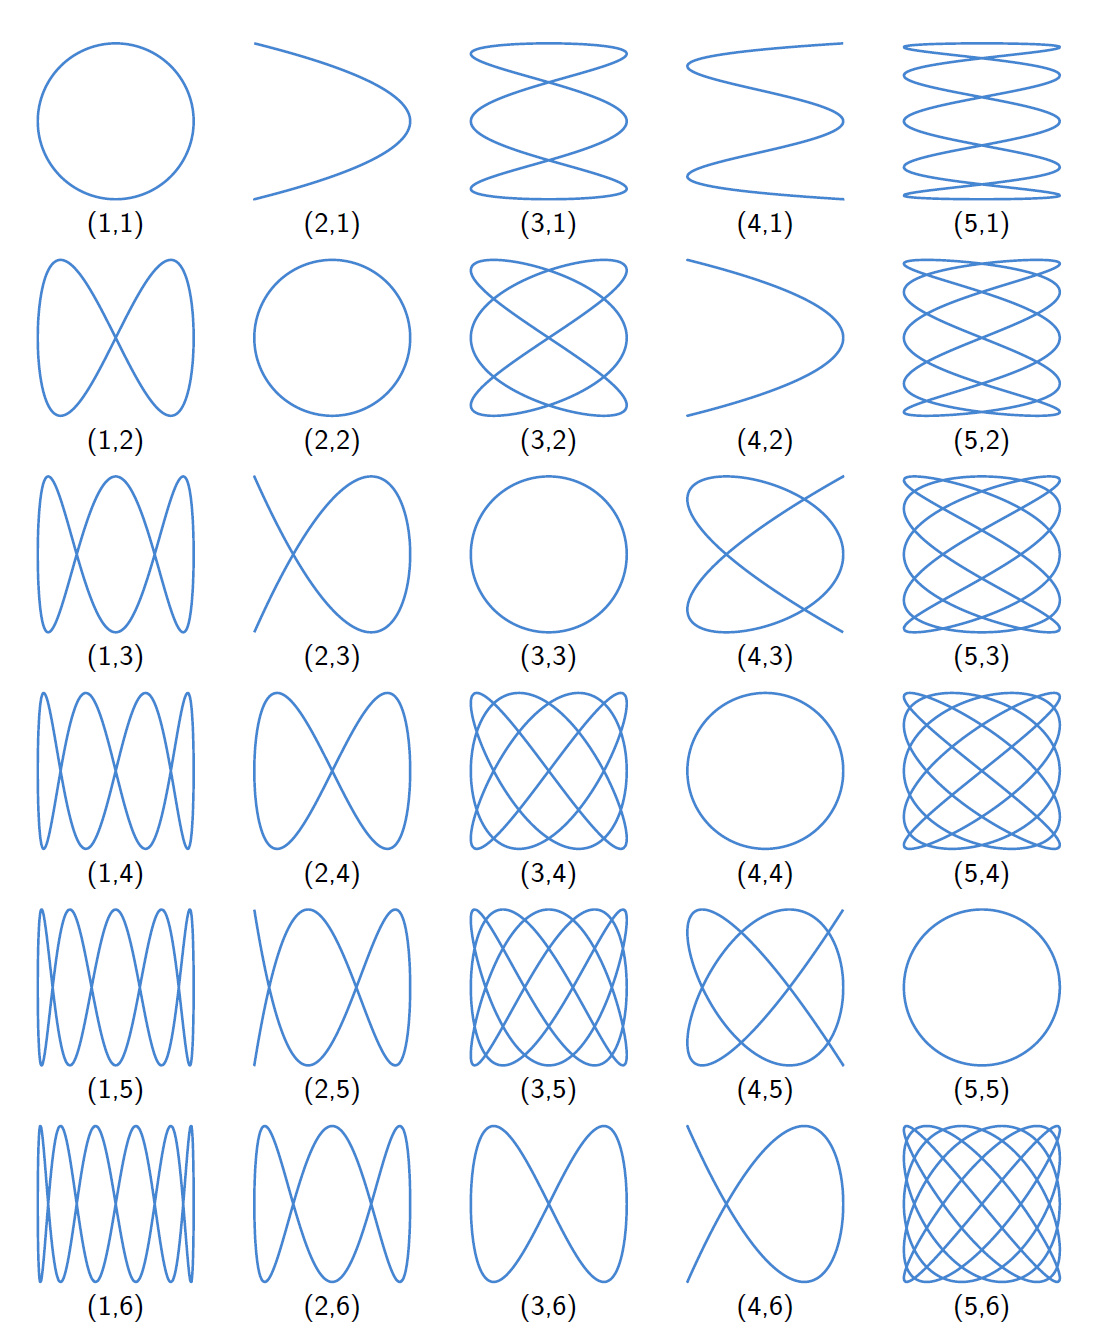
\includegraphics[width=11cm]{images/planche.jpg}%
}
\caption{Exemples de fonctions paramétriques}
\end{center}
\end{figure}


\section{Tikz} \label{tikz} %\incise{---}{---}{---}

Le paquet \paquet{tikz} est plus récent que le paquet \paquet{pstricks}. Par rapport à ce dernier, il présente deux avantages :
\begin{itemize}
\item il dispose généralement de plus grandes possibilités de paramétrages ;
\item il fonctionne avec les différentes chaînes générant directement des fichiers \dextension{pdf}, ce qui en fait la solution graphique pour les fichiers image \dextension{jpg} mais aussi avec les variantes de \LaTeX{} que sont \XeLaTeX{} et Lua\LaTeX.
\end{itemize}

En contrepartie, il demande un peu plus de temps pour être utilisé. Par ailleurs, sur des graphiques nécessitant des calculs, il est plus lent que \paquet{pstricks}, ce dernier bénéficiant des mécaniques propres au langage postscript.

Ce paquet met à disposition un environnement pour traiter les figures : 
\begin{codesimple}{L'environnement de \pseudopaquet{tikz}}{environnementtikz}
\begin{tikzpicture}[§oc£¤options§fc] 
% Figure tikz
\end{tikzpicture}
\end{codesimple}


Cet environnement ne nécessite pas, contrairement à celui de \paquet{pstricks} de dimension : \paquet{tikz} va déterminer les dimensions de la zone à afficher pour qu'elle contienne et affiche l'ensemble des objets tracés\footnote{Ce comportement peut se piloter. Il suffit de placer des n\oe{}uds délimitant une zone plus large pour forcer \paquet{tikz} à suivre d'éventuels besoins de présentation.}. Qui plus est, \paquet{tikz} prend en compte d'éventuelles\textit{options} : ces dernières vont s'appliquer à l'ensemble des objets décrits par la suite, sauf règle explicite contraire présente dans un objet ou une classe d'objets.

\subsection{Le placement par les n\oe{}uds}

Sous \paquet{tikz}, les éléments sont placés sur un n\oe ud (\emph{node}). Un n\oe ud peut être défini par des coordonnées ou de façon relative à d'autres points. Il peut également être appelé par son nom.

\codefigure{
\macro{begin}\{tikzpicture\}[outer sep=0cm,inner sep=0cm] \\
\macro{node} (aa) at (1,0.5) \{1.\macro{LaTeX}\}; \\
\macro{node} (ab) at (0.8,1.1) \{\}; \\
\macro{node}[anchor=south west] at (ab) \{\macro{resizebox}\{3.5cm\}\{!\}\{2.\macro{textcolor}\{bleu5\}\{\macro{LaTeX}\}\}\}; \\
\macro{node}[rotate=160] (ac) at (8,1.1) \{\macro{resizebox}\{!\}\{0.7cm\}\{3.\macro{LaTeX}\}\}; \\
\macro{node} (ad) at (6,1) \{\}; \\
\macro{node}[anchor=north east,outer sep=0cm,inner sep=0cm] at (ad) \{\macro{resizebox}\{!\}\{0.6cm\}\{\macro{reflectbox}\{4.\macro{LaTeX}\}\}\}; \\
%\draw[color=bleu6] plot[only marks,mark=x] coordinates{(aa)(ab)(ac)(ad)};
\macro{end}\{tikzpicture\}
}{
\fontfamily{lmr}\selectfont
\begin{tikzpicture}[outer sep=0cm,inner sep=0cm]
\node (a) at (0,0) {}; \node (b) at (10,2) {}; % pour dimensionner l'image
\node (aa) at (1,0.5) {1.\LaTeX};
\node (ab) at (0.8,1.1) {};
\node[anchor=south west] at (ab) {\resizebox{3.5cm}{!}{2.\textcolor{bleu5}{\LaTeX}}};
\node[rotate=160] (ac) at (8,1.1) {\resizebox{!}{0.7cm}{3.\LaTeX}};
\node (ad) at (6,1) {};
\node[anchor=north east,outer sep=0cm,inner sep=0cm] at (ad) {\resizebox{!}{0.6cm}{\reflectbox{4.\LaTeX}}};
\draw[color=bleu6] plot[only marks,mark=x] coordinates{(aa)(ab)(ac)(ad)};
\end{tikzpicture}
}{Placements et redimensionnements}

\subsection{Les boîtes ou formes}

Différentes formes sont prédéfinies sous \paquet{tikz}\footnote{en particulier avec la bibliothèque \emph{shape} qui définit par exemple le losange utilisé dans l'exemple.}. Se retrouve ici la logique de préciser le tracé du pourtour, le remplissage de la forme, la présence d'une ombre, que ce soit pour la couleur, l'épaisseur, les motifs...). 

De nombreuses valeurs sont disponibles sous forme de mots clés. Par exemple, \macron{thick} utilisé dans l'exemple définit un trait de 0,8pt d'épaisseur.

\codefigure{
\macro{begin}\{tikzpicture\} \\
\macro{node}[rectangle,draw] at (2,1) \{1.\macro{LaTeX}\}; \\
\macro{node}[rectangle,fill=bleu6,drop shadow] at (5,0.5) \{2.\macro{LaTeX}\}; \\
\macro{node}[diamond,aspect=2.5,draw=bleu6,thick] at (5,1.5) \{3.\macro{LaTeX}\}; \\
\macro{node}[circle,draw=bleu6,loosely dotted,thick] at (8,1) \{\macro{Large} 4.\macro{LaTeX}\}; \\
\macro{end}\{tikzpicture\}
}{
\fontfamily{lmr}\selectfont
\begin{tikzpicture}%[outer sep=0cm,inner sep=0cm]
\node (a) at (0,0) {}; \node (b) at (10,2) {}; 
\node[rectangle,draw] at (2,1) {1.\LaTeX}; 
\node[rectangle,fill=bleu6,drop shadow] at (5,0.5) {2.\LaTeX}; 
\node[diamond,aspect=2.5,draw=bleu6,thick] at (5,1.5) {3.\LaTeX}; 
\node[circle,draw=bleu6,loosely dotted,thick] at (8,1) {\Large 4.\LaTeX}; 
\end{tikzpicture}
}{Boîtes}

\subsection{Les grilles}

Les grilles se présentent sous une forme un peu différente de celle vue dans \paquet{pstricks}. En effet, la fonctionnalité la plus courante ne propose pas la numérotation des axes ; de même la grille se base sur les coordonnées du plan ce qui fait que la seconde grille ci-dessous ne commence pas par un filet vertical. 

\begin{codedoublefig}{Grilles}{tikzgrilles}
\begin{tikzpicture}%[outer sep=0cm,inner sep=0cm]
\node (a) at (0,0) {}; \node (b) at (10,2) {}; 
\draw[step=.2cm,gray,very thin] (0,0) grid (2,1.4);
\draw[step=1cm] (0,0) grid (2,1.4);
\draw (3.5,0) grid[xstep=0.4cm,ystep=0.5cm] (5.5,1.4);
\end{tikzpicture}
\end{codedoublefig}

Par contre, lorsqu'il s'agit de traiter la représentation de données, \paquet{tikz} dispose de commandes avancées pour traiter ce point.

\subsection{Les points et courbes}

De la même manière, \paquet{pstricks} dispose de plusieurs commandes de base pour former des traits anguleux, curvilignes. L'exemple suivant les présente sans option.

\begin{codedoublefig}{Points et courbes}{tikzpoints}
\begin{tikzpicture}%[outer sep=0cm,inner sep=0cm]
\node (a) at (0,0) {}; \node (b) at (10,2) {}; 
\fill (0,1) circle (2pt);
\fill (0.5,0) circle (2pt);
\fill (1,0.5) circle (2pt);
\fill (1.5,0) circle (2pt);
\fill (2,1) circle (2pt);
\draw (2.5,1) -- (3,0) -- (3.5,0.5) -- (4,0) -- (4.5,1);
\draw plot[smooth] coordinates{(5,1) (5.5,0) (6,0.5) (6.5,0) (7,1)};
\draw plot[smooth cycle,tension=0.8] coordinates{(7.5,1) (8,0) (8.5,0.5) (9,0) (9.5,1)};
\end{tikzpicture}
\end{codedoublefig}


\alerte{Présentation à poursuivre}


%%%%%%%%%%%%%%%%%%%%%%%%%%%%%%%%%%%%%%%%
%%%%%  Chapitre Polices de caractère
%%%%%%%%%%%%%%%%%%%%%%%%%%%%%%%%%%%%%%%%

\chapter{Les polices de caractères avec \XeLaTeXtitre}
\index[con]{polices de caractères} \label{fontes} \label{xelatex}

La méthode de gestion d'autres polices de caractères présentée page \pageref{carac} est limitée dans ces possibilités. Il en existe une autre, plus complexe mais \emph{très} efficace et qui passe par l'utilisation de variantes récentes de \TeX : \XeTeX\ (et \XeLaTeX) qui rend plus intuitive l'utilisation de polices de caractères en donnant accès direct à l'ensemble des fontes utilisées par Windows ou MacOS.

\section{Modifications associées à \XeLaTeXtitre}

Pour utiliser \XeLaTeX, il faut vérifier que le préambule est bien cohérent avec la version présentée en page \pageref{xelualatex}. La déclaration d'un jeu particulier de polices de caractères se fait ensuite par la commande suivante.

\begin{codesimple}{Création d'une famille de polices de caractères}{creationpolice}
\newfontfamily\§oc£¤mapolice §fc[
 BoldFont = §oc policegrasse.ttf §fc,
 ItalicFont = §oc policeitalique.ttf §fc,
 BoldItalicFont = §oc policeitaliquegrasse.ttf §fc
 ]{§oc policenormale.ttf §fc}
\end{codesimple}

La commande est donnée dans une version détaillée permettant de bénéficier de certaines fonctionnalités courantes. \XeLaTeX\ peut attendre d'une police de caractères qu'elle présente quatre versions : une normale, une variante grasse, une variante italique et une variante italique grasse. Certaines polices de caractères présentent naturellement ces quatre variantes, d'autres pas. Aussi la commande peut donc être parfois moins détaillée. 

Les noms indiqués en italique correspondent aux noms des fichiers de polices de caractères nous intéressant et présents dans le répertoire usuel du système d'exploitation\footnote{Il s'agit de \vue{C:\ba Windows\ba Fonts} pour Windows.}: ce peut être des fichiers \dextension{ttf} ou \dextension{otf}.

Pour utiliser ces polices dans le document, il suffit d'utiliser la nouvelle bascule mise à disposition par la commande, ici \macro{mapolice}. 

Dans le cas où il faut modifier les polices de caractères utilisées par défaut par \LaTeX, il est fait usage d'une autre  commande à la syntaxe similaire.

\begin{codesimple}{Mise en valeur par défaut d'une famille de polices de caractères}{policedefaut}
\setmainfont[Path=fontes/,
 BoldFont = §oc policegrasse.ttf §fc,
 ItalicFont = §oc policeitalique.ttf §fc,
 BoldItalicFont = §oc policeitaliquegrasse.ttf §fc
 ]{§oc policenormale.ttf §fc}
\end{codesimple}

La commande est ici présentée avec l'option \macron{Path} qui permet d'indiquer un chemin où trouver les fichiers des polices de caractères. Cette commande gère la fonte principale et ses variantes. Si une variante sans serif existe, elle peut être également déclarée avec \macro{setsansfont} avec les mêmes options.

\section{Pour aller plus loin}

Il est ici recommandé de consulter la documentation de \paquet{fontspec} pour mieux appréhender les possibilités de ce paquet. Un point doit être cependant conserver à l'esprit : la manipulation de polices de caractère devrait être limitée pour des documents longs car ceci peut involontairement conduire à des documents relativement peu lisibles et souvent contraires à certains usages typographiques.

Plus largement, le logiciel \programme{FontForge}\footnote{\liensimple{http://fontforge.github.io/en-US/}.}, libre, permet d'éditer des polices de caractères, ne serait-ce par exemple que pour créer de façon quasi-automatique des petites capitales sur des polices de caractères existantes.
%%%%%%%%%%%%%%%%%%%%%%%%%%%%%%%%%%%%%%%%
%%%%%  Chapitre Extension maison
%%%%%%%%%%%%%%%%%%%%%%%%%%%%%%%%%%%%%%%%

\chapter{Un fichier d'extension}

Un paquet ou extension est un fichier d'extension \dextension{sty} regroupant des ensembles de définitions permettant de modifier et d'élargir les traitements qu'effectue \LaTeX. Ce chapitre décrit la structure d'un tel fichier.

\section{Déclarations}

Afin d'être traité correctement par \LaTeX\ et par les différentes mécaniques associées à la distribution, ce fichier contient quelques commandes de description du paquet, placées en début de fichier :

\begin{codesimple}{Déclaration d'un paquet}{codextensionmin}
\NeedsTeXFormat{LaTeX2e}
\ProvidesPackage{§textit£nompaquet¤}[§textit£aaaa/mm/jj version et autres infos¤]
\end{codesimple}

Le format de la date (\emph{aaaa/mm/jj}) est normalisé mais le reste de la description est libre.

\section{Options}

\subsection{Déclaration des options}

L'appel d'un paquet peut se faire avec des options, comme vu en \ref{toto}, page~\pageref{toto}. Chacune des options est en fait un code présent dans le fichier du paquet. Ce \emph{code} est rattaché au terme \emph{nomoption}, le nom de l'option, et est à déclarer par la commande suivante :

\begin{codesimple}{Déclaration et définition d'une option}{codextensionoption}
\DeclareOption{§textit£nomoption¤}{§textit£code¤}
\end{codesimple}

\subsection{Traitement des options}

Une des options ainsi déclarée peut être considéré comme l'option par défaut. Dans ce cas, après avoir déclaré les différentes options, la commande suivante permet d'exécuter systématiquement le code des options listées (séparées par des virgules). 

\begin{codesimple}{Exécution d'options listées}{codextensionexecute}
\ExecuteOptions{§textit£liste d'options¤}
\end{codesimple}

Pour traiter le choix d'options fait par l'utilisateur et exécuter les codes associés, il faut alors placer la commande suivante.

\begin{codesimple}{Exécution des options appelées par l'utilisateur}{codextensionprocess}
\ProcessOptions \relax
\end{codesimple}

\subsection{Transmission d'options}

Dans le code contenu dans une commande \macro{DeclareOption}, il est possible d'indiquer des options à transmettre à un paquet appelé par la suite dans l'extension. 

\begin{codesimple}{Transmission d'options}{codextensionpass}
\PassOptionsToPackage{§textit£liste d'options¤}{§textit£paquet¤}
\end{codesimple}

\section{Appel d'autres paquets}

Certaines définitions ou fonctionnalités demandent à charger d'autres paquets. Pour cela, il ne faut pas utiliser la commande \macro{usepackage} mais une commande spécifique aux fichiers d'extension : 

\begin{codesimple}{Appel de paquet}{codextensionpaquet}
\RequirePackage[§textit£options¤]{§textit£paquet¤}
\end{codesimple}


\section{Codes particuliers}

Certains éléments d'un paquet peuvent demander des exécutions à des moments particuliers. Quelques commandes sont associés à trois moments de la compilation : à la fin de l'exécution du code du paquet, au début du corps du document ou à fin du document. Elles stockent le code pour exécution au moment qu'elles indiquent.

\begin{codesimple}{Stockage de code pour exécution à des moments spécifiques}{codextensionat}
\AtEndOfPackage{§textit£code¤}
\AtBeginDocument{§textit£code¤}
\AtEndDocument{§textit£code¤}
\end{codesimple}

Ces commandes peuvent être utilisées à plusieurs reprises : les codes qu'elles contiennent s'empilent alors en vue de l'exécution au moment associé.

Par ailleurs, la commande \macro{AtBeginDocument} est considérée comme appartenant au préambule du document et non au corps. Elle ne peut donc contenir de texte.

\section{Exemple}

Voici un exemple de code d'un paquet \macron{demo}.

\begin{codesimple}{Exemple}{codextensionexemple}
\NeedsTeXFormat{LaTeX2e}
\ProvidesPackage{demo}[1902/01/17 V1.0 Quelques chargements]

% Déclaration des options
\DeclareOption{defaut}{%
\newcommand{\signature}{\textit{Signature}}%
}

\DeclareOption{perso}{%
\newcommand{\signatureab}{Ambrose \textsc{Bierce}}%
\PassOptionsToPackage{dvipsnames}{xcolor}%
}

% Traitement des options
\ExecutesOption{defaut}
\ProcessOptions \relax

% Appels de paquets et définitions communes
\RequirePackage{xcolor}
\RequirePackage{xspace}
\newcommand{\MonLaTeX}{\LaTeX\xspace}
\end{codesimple}

Ce paquet dispose de deux options : \macron{defaut} et \macron{perso}. La première option est exécutée par défaut avec la commande \macro{ExecutesOption} et crée une commande \macro{signature}. La seconde option n'est exécutée que si le paquet \macron{demo} est appelé avec l'option \macron{perso}. Est alors définie une commande \macro{signatureab}. De plus, il est demandé de passer une option complémentaire au paquet \paquet{xcolor} lorsque ce dernier sera appelé : \macron{dvipsnames}. 

Une fois les options traitées, ce paquet appelle le paquet \paquet{xcolor} et le paquet \paquet{xspace}. L'option \macron{perso} aura ici modifié le premier appel en lui ajoutant l'option \macron{dvipsnames}.

Enfin, une fonction \macro{MonLaTeX} est définie.


\section{Pour aller plus loin}

Il est également possible de créer des classes de document (fichiers \dextension{cls} sur des principes très similaires. Point non signalé ci-dessus, il est également possible d'inclure des textes d'erreur à afficher si une erreur survient. Ces deux éléments sont décrits dans cette documentation en anglais : \liensimple{http://www.latex-project.org/guides/clsguide.pdf}.

Il est également possible de faire un travail plus complet en créant des fichiers qui génèrent à la fois le code du paquet (ou de la classe), la documentation générale et la documention du code. La méthode est présentée dans un document en français : \liensimple{http://yvon-henel.fr/texnicien/docs/dtxtut-fr/dtxtut-fr.pdf}.

%%%%%%%%%%%%%%%%%%%%%%%%%%%%%%%%%%%%%%%%
%%%%%  Chapitre PythonTeX
%%%%%%%%%%%%%%%%%%%%%%%%%%%%%%%%%%%%%%%%

\chapter{Python\TeX}

\section{Brève présentation du langage}

\alerte{\`{A} compléter}

Le langage Python est un langage interprété (pas besoin de compilation) généraliste. Son principal avantage est la lisibilité du code ainsi que la multitude d'exemples disponibles en ligne en matière de traitement de données, notamment.

Pour installer Python et un ensemble de modules très complet, il suffit d'utiliser la distribution anaconda : celle-ci comporte la plupart des modules nécessaires au calcul scientifique et au traitement de données.

Le package Python\TeX permet d'utiliser des résultats de programmes python et de les insérer au sein d'un document \LaTeX.

L'intérêt d'une telle technique réside dans la création de documents dont les résultats peuvent être mis à jour automatiquement.

\section{Calcul scientifique}

\alerte{\`{A} compléter}


\section{Exemples d'utilisation}

\alerte{\`{A} compléter}
Did you know that $2^{65} = \py{2**65}$ ?

\begin{pycode}
print(r"\begin{tabular}{c|c}")
print(r"$m$ & $2^m$ \\ \hline")
print(r"%d & %d \\" % (1, 2**1))
print(r"%d & %d \\" % (2, 2**2))
print(r"%d & %d \\" % (3, 2**3))
print(r"%d & %d \\" % (4, 2**4))
print(r"\end{tabular}")
\end{pycode}

\section{Pour aller plus loin}

\alerte{\`{A} compléter}



%%%%%%%%%%%%%%%%%%%%%%%%%%%%%%%%%%%%%%%%
%%%%%  Annexes
%%%%%%%%%%%%%%%%%%%%%%%%%%%%%%%%%%%%%%%%

\part{Annexes}
\appendix                              % Passage aux notations "annexe"
%%%%%%%%%%%%%%%%%%%%%%%%%%%%%%%%%%%%%%%%
%%%%%  Chapitre Installation
%%%%%%%%%%%%%%%%%%%%%%%%%%%%%%%%%%%%%%%%

\chapter{Installation}  \index[con]{installation}

Les installations présentées ici sont sous Windows. Pour une installation Mac, il convient de consulter le document de Fabien \textsc{Conus} et de Franck \textsc{Pastor}\cite{conu}.

L'installation de \LaTeX\ est très fortement marquée par l'aspect modulaire de ce programme : beaucoup de fichiers sont créés et dépendent les uns des autres. Par ailleurs, \LaTeX\ crée par défaut des documents affichables mais non imprimables. L'installation de certains programmes complémentaires permet de convertir ces documents dans des formats imprimables. 


\section{Une installation compacte : USB\TeX}

L'installation retenue pour le cours est USB\TeX\ du fait de sa simplicité d'utilisation. Il s'agit d'un regroupement de plusieurs programmes de taille réduite : la distribution (voir ci-dessous) MiK\TeX, les programmes \programme{Ghostscript}, \programme{GSview} et l'éditeur \programme{Texmaker}.

\subsection{Installation}

Le fichier exécutable d'un peu plus de 150~Mo est téléchargeable par le biais du site de Framasoft\footnote{\liensimple{http://www.framasoft.net/article4641.html}. S'y trouve également le mode d'emploi résumé ci-dessus.}. L'exécution de ce fichier le fait se décompresser dans le répertoire demandé par la fenêtre qui s'affiche alors. Ceci fait, il faut se placer dans le répertoire nouvellement créé par l'installation\footnote{Ce répertoire est nommé \vue{USBTeX-} suivi du numéro de version d'USB\TeX.} et cliquer sur le raccourci nommé  \vue{Texmaker} pour pouvoir utiliser l'éditeur \programme{Texmaker}.  

\subsection{Maintenance}

\subsubsection{Cas usuel}

L'installation initiale faite ci-dessus inclut un nombre restreint de paquet. Si, lors d'une compilation, un paquet semble manquant pour l'installation, \programme{Texmaker} vous propose de l'installer directement par téléchargement en ligne (en passant par le logiciel de maintenance de MiK\TeX). Ceci évite de se poser des questions concernant les paquets, leur installation et leur maintenance. 

\subsubsection{Cas moins usuel}

L'installation de paquet peut aussi se faire de façon plus manuelle en allant directement installer les paquets souhaités. Pour le faire, il faut lancer le raccourci \vue{MiKTeX} présent dans le répertoire créé par l'installation. 

Ceci fait apparaître une nouvelle icône dans la barre des tâches. En cliquant avec le bouton droit dessus et en sélectionnant \vue{MiKTeX Package Manager} se lance alors le gestionnaire de paquet. Il peut mettre un certain temps avant de réagir car il compare les paquets présents et les paquets disponibles. Une fois la liste des paquets affichée, il suffit de sélectionner ici n'importe quel paquet et de cliquer sur l'icône \vue{+} pour l'installer.

\subsubsection{Cas improbable mais vrai}

Il peut arriver que des problèmes de configuration de connexion empêche d'utiliser ce système directement. Si la connexion internet est fonctionnelle, il est possible de contourner cette difficulté en récupérant soi-même les fichiers que va chercher le gestionnaire de paquets sur des dépôts (\emph{repository} en anglais) et en les stockant dans un répertoire dédié sur son ordinateur. 

Une fois connue l'adresse d'un dépôt\footnote{Par exemple \liensimple{ftp://ftp.dante.de/pub/tex/systems/win32/miktex/tm/packages/}. Une liste de dépôts est disponible à l'adresse \liensimple{http://miktex.org/pkg/repositories}.}, il faut alors y récupérer et placer dans un unique répertoire de son ordinateur les éléments suivants :
\begin{itemize}
\item les fichiers dont le nom commence par \vue{miktex-zzdb} ;
\item les fichiers des paquets qui vous intéressent.
\end{itemize}

Le premier ensemble de fichiers sert à indiquer la liste des paquets du dépôt au gestionnaire de paquet. En l'absence de ces fichiers, le gestionnaire de dépôt refusera de prendre en compte votre répertoire.

Dans le gestionnaire de paquet MiK\TeX, il faut alors aller dans le menu \vue{Repository} puis \vue{Change Package Repository}, sélectionner alors la ligne \vue{... from a directory} puis \vue{Suivant}, sélectionner le répertoire où sont vos paquets et cliquer enfin sur \vue{Terminer}.

\subsection{La vérification orthographique}

L'installation sur clé présente une coquille pour ce qui est du correcteur orthographique. Il faut modifier le chemin présent dans le menu \vue{Options}, \vue{Configurer Texmaker} puis \vue{Editeur}. Le chemin de la ligne \vue{Dictionnaire} est à modifier par le biais de la petite icône à côté de la zone de saisie du chemin, en cherchant le répertoire où est installé USBTeX (\vue{USBTeX-1.7}) puis en allant dans le sous-répertoire \vue{programs} puis \vue{Texmaker} et sélectionner alors le fichier \vue{fr\_FR.dic}. 

\section{Une installation complète}

Le côté pratique d'USB\TeX\ cache les liens entre les différents programmes. Est donc décrite ici une installation complète\footnote{Parmi d'autres possibles telle \liensimple{http://www.xm1math.net/doculatex/install_miktex.html}.} sous Windows. Celle-ci demande de récupérer trois ensembles :
\begin{itemize}
\item une \terme{distribution} de \LaTeX, autrement dit \LaTeX\ et de nombreux programmes et fichiers satellites (paquets, documentations, formats...) ;
\item \programme{Ghostscript} et \programme{GSview} qui gèrent le postscript et les fichiers \dextension{ps} et \dextension{eps} ;
\item un éditeur \LaTeX, point vu en section \ref{éditeurs}.
\end{itemize}

% install-tl-windows.bat
\subsection{\LaTeX}

La distribution retenue ici de \LaTeX\ est la \TeX Live 2014, soumise à la licence GNU\footnote{Licence qui gère le logiciel libre.}. La dernière distribution de la \TeX live est disponible sur \liensimple{http://www.tug.org/texlive/}. Plusieurs modes d'installation sont possibles :
\begin{itemize}
\item en téléchargeant un fichier d'installation qui récupère les différents fichiers nécessaires sur le web. Il se trouve sur le site en suivant le lien \vue{Download} puis le lien \vue{install-tl.zip}.\index[con]{texlive@\TeX Live} Une fois ce fichier décompressé, il faut exécuter le programme \vue{install-tl.bat}, qui affiche la fenêtre de la figure \ref{figtexlive} ;
\item en téléchargeant le DVD d'installation présent sur le site\footnote{Actuellement, l'adresse donnée est la suivante : \liensimple{http://mirrors.ircam.fr/pub/CTAN/systems/texlive/Images/texlive2014-20140525.iso}.}. Ce fichier doit alors être gravé ou monté sur un lecteur virtuel. Une fois lancé, il faut lancer le fichier \vue{install-tl-windows.bat} qui affiche le même menu qu'à la méthode précedente.
\end{itemize}

\begin{figure}[H]
\centering 
\resizebox{10cm}{!}{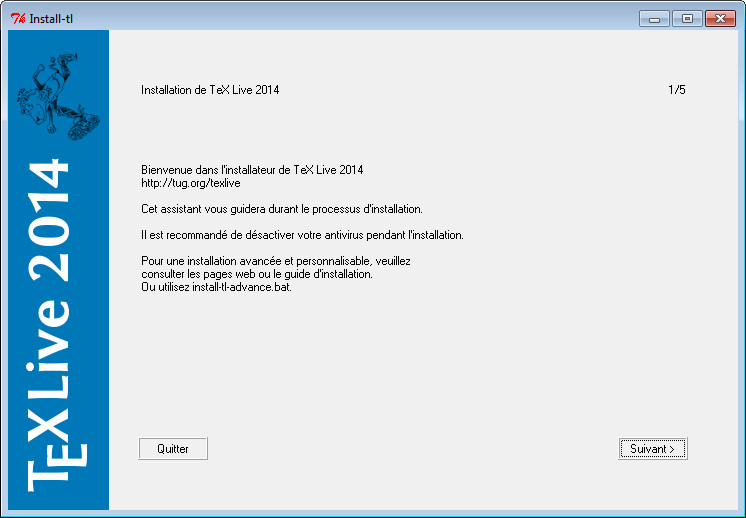
\includegraphics{images/texlive2014.jpg}}
\caption{Page d'accueil de \TeX Live 2014}\label{figtexlive}
\end{figure}

Les différents choix usuels de configuration sont récapitulés dans le tableau suivant à raison d'une ligne par fenêtre d'installation.

\begin{table}[H]
\centering
\begin{tablecouleur}
\begin{tabular}{cl}
\rowcolor{bleu20}
\color{white}\bf Fenêtre &  \multicolumn{1}{c}{\color{white}\bf Action}	\\ 
1/5 & Suivant 															\\ 
2/5 & Répertoire \vue{C:\ba TeXLive\ba 2014}. Suivant 	\\
3/5 & Suivant 															\\ 
4/5 & Installer 														\\ 
5/5 & Attendre et quitter 												\\
\end{tabular}
\end{tablecouleur}
\caption{\'{E}tapes d'installation de la \TeX live 2014}
\end{table}

Cette partie est assez longue, surtout si c'est la méthode du fichier d'installation qui est retenue : les différents fichiers constitutifs de l'installation seront tous téléchargés. Dans la mesure où il y a beaucoup de fichiers de taille variable, la durée de téléchargement est elle-même délicate à mesurer. Par expérience, il faut compter deux bonnes heures. 

Avec la méthode par DVD, le temps d'installation passe environ à une demi-heure.

\subsection{\programme{Ghostscript} et \programme{GSview}}
\subsubsection{\programme{Ghostscript}} 

\programme{Ghostscript} permet de travailler avec des fichiers postscript ou \dextension{ps} ainsi que les images au format \dextension{eps}. Avec le programme \programme{ps2pdf} compris dans les programmes fournis avec \programme{Ghostscript}, il devient possible de convertir un fichier \dextension{ps} en \dextension{pdf}. 

Une fois le programme dans sa version libre non commerciale (nommée GPL ou \emph{General Public License}) téléchargé\footnote{Il se trouve à l'adresse \liensimple{http://www.ghostscript.com/download/gsdnld.html}.}, il convient de suivre la suite d'instructions présentée ci-après.

\begin{table}[H]
\centering
\begin{tablecouleur}
\begin{tabular}{cl}
\rowcolor{bleu20}
\color{white}\bf Fenêtre 	& \multicolumn{1}{c}{\color{white}\bf Action}		\\ 
Welcome						& Next    											\\ 
License agreement			& I agree 											\\
Choose install				& Répertoire \vue{C:\ba Texlive\ba gs}. Install		\\
Completing					& Finish 											\\
\end{tabular}
\end{tablecouleur}
\caption{\'{E}tapes d'installation de \programme{Ghostscript}}
\end{table}


\subsubsection{\programme{GSview}}
  
\programme{GSview} est un outil graphique qui facilite grandement l'utilisation de \programme{Ghostscript}. Grâce à lui, la visualisation d'un document \dextension{ps} est simplifiée. 

La version de \programme{GSview} à télécharger\footnote{À l'adresse \liensimple{http://pages.cs.wisc.edu/~ghost/gsview/index.htm}, en retenant par rapport à la remarque ci-dessus la version \vue{GSview release v5.0}.} doit être compatible avec la version de \programme{Ghostscript}. Une fois lancé l'exécutable, les étapes de configuration sont indiquées ci-après.

\begin{table}[H]
\centering
\begin{tablecouleur}
\begin{tabular}{cl}
\rowcolor{bleu20}
\color{white}\bf Fenêtre 	& \multicolumn{1}{c}{\color{white}\bf Action}			\\ 
Winzip Self-Extractor	 	& Setup     											\\
Select Language 			& Francais 												\\
This wizard will		 	& Next		   											\\
Copyright					& Next   												\\
GSview can create	 		& Next	   												\\
Select a directory			& Répertoire \vue{C:\ba Texlive\ba Ghostgum}. Next		\\
The directory you			& Next		   											\\
GSview setup will			& Finish	  											\\
Installation successful		& Exit 													\\
\end{tabular}
\end{tablecouleur}
\caption{\'{E}tapes d'installation de \programme{GSview}}
\end{table}

Point important, il faut lancer une première fois \programme{GSview} pour le configurer. Sans cela, il indiquera systématiquement une erreur à l'ouverture d'un fichier \dextension{ps}. Une fois lancé, il faut aller dans le menu \vue{Options} puis \vue{Easy Configure} et sélectionner le numéro de version de \programme{Ghostscript}\footnote{Ce dernier est dans le nom du fichier d'installation de \programme{Ghostscript}.}. \programme{GSview} peut alors être fermé.


\subsection{Configuration de Windows}

Les différentes versions de Windows réagissent diversement à l'installation de \LaTeX. La plupart des versions\footnote{Windows 7 semble faire exception.} ne feront pas fonctionner \programme{ps2pdf}, mystérieusement introuvable. Il faut comprendre par là que lorsque Windows cherche un programme, il parcourt une liste de répertoires bien spécifiques et, dans notre cas, nos répertoires contenant \LaTeX\ ou \programme{Ghostscript} n'en font pas partie.

Pour corriger ce point, il faut modifier la variable \vue{Path} des variables d'environnement. Dans le panneau de configuration, double-cliquer sur \vue{Système}\footnote{Dans le cas de Windows XP, il faut d'abord cliquer sur l'icône \vue{Performance et maintenance}. Pour Windows Vista, il faut demander l'affichage \og classique \fg, l'icône \vue{Système} apparaissant alors.}. Sélectionner alors l'onglet avancé et cliquer alors sur \vue{Variables d'environnement}. 

\begin{figure}[H]
\centering
\resizebox{10cm}{!}{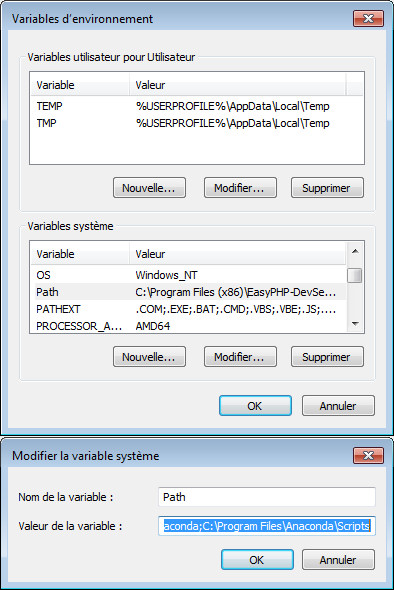
\includegraphics{images/variables.jpg}}
\caption{Exemple d'entrée des chemins sous Windows XP}
\end{figure}

Là, il faut sélectionner la ligne \vue{Path} et cliquer sur \vue{Modifier}. On ajoute alors\footnote{... sans effacer les chemin déjà présents !} les chemins vers nos programmes, autrement dit la ligne suivante\footnote{Les points-virgules servent ici de séparateurs entre les différents chemins.} :
\begin{center}
\vue{\footnotesize\texttt{;C:\ba Texlive\ba bin\ba win32\ba;C:\ba Texlive\ba gs\ba gs9.06\ba bin\ba;C:\ba Texlive\ba gs\ba gs9.06\ba lib\ba}}
\end{center}


\section{Des éditeurs} \label{éditeurs}

Une fois les différents programmes fondamentaux installés, il faut installer un programme permettant d'éditer de façon simple les documents \dextension{tex} et de lancer aisément des compilations ou des conversions de document. Ce document en présente deux. 

Dans tous les cas, un point d'attention est porté sur la configuration car il faut systématiquement indiquer à ces programmes où se trouvent les différents programmes que nous avons installé précédemment.


\subsection{\programme{Texmaker}}

Programme libre sous licence GNU, \programme{Texmaker}\footnote{Il est téléchargeable à l'adresse \liensimple{http://www.xm1math.net/texmaker/index_fr.html}.} est un des logiciels de référence pour l'édition de documents \dextension{tex}. L'installation se limite tout au mieux à indiquer le répertoire où sera installé le programme. Le paramétrage des programmes s'obtient par le menu \vue{Options}, \vue{Configurer Texmaker}. L'image ci-dessous\footnote{Cette présentation dépend de la version de \programme{Texmaker} mais contient le même type d'information.} donne la configuration attendue par défaut.

\begin{figure}[H]
\centering
\resizebox{14cm}{!}{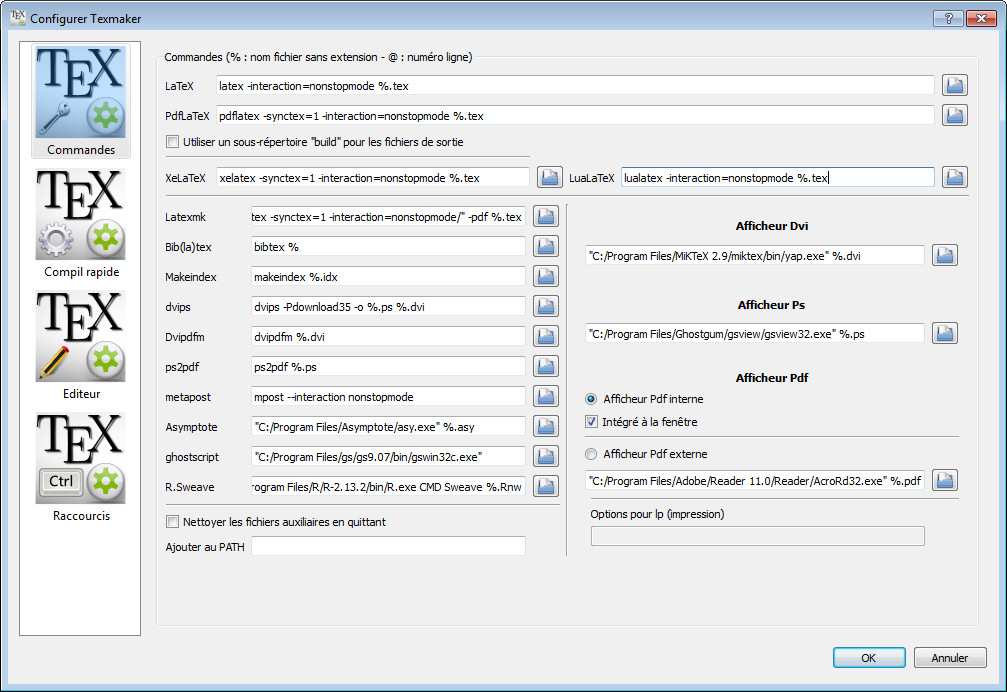
\includegraphics{images/texmaker441.jpg}}
\caption{Paramétrage de \programme{Texmaker}}
\end{figure}

\programme{Texmaker} gère l'encodage UTF8. Il s'agit d'une norme de saisie des caractères qui se répand de plus en plus car elle permet de gérer de très nombreuses langues. Si vous utilisez UTF8, il faut modifier le préambule de notre document, en remplaçant \macron{latin1} par \macron{utf8}. 

\begin{codesimple}{Code pour l'UTF8}{codeutf}
\usepackage[utf8]{inputenc}
\end{codesimple}

Selon la version de \programme{Texmaker}, la gestion de l'UTF8 n'est pas systématique. Il faut parfois modifier directement l'encodage utilisé par défaut. Ceci se fait dans le menu \vue{Options}, \vue{Configurer Texmaker}, \vue{Editeur} en paramétrant dans l'encodage \vue{UTF-8}.

\subsection{\programme{TeXnicCenter}}

\programme{TeXnicCenter}\footnote{Téléchargeable à l'adresse \liensimple{http://www.texniccenter.org/}.} offre une large panoplie de fonctionnalités, à l'image de \programme{Texmaker}. L'installation propose un peu plus de choix que dans \programme{Texmaker} et demande également la localisation des fichiers de la distribution\footnote{Il faut indiquer le répertoire \vue{C:\ba Texlive\ba 2014\ba bin\ba win32} si vous avez suivi le paramétrage proposé dans ce document.}. Les options proposées restent lisibles et rendent cette phase peu difficile. 

L'installation vous demandant de lui indiquer où est la distribution, il n'y a pas ou peu d'actions à faire pour configurer \programme{TeXnicCenter}. \`{A} titre d'information,  cette opération se fait dans le menu \vue{Build} puis \vue{Define Output Profiles}. 

\begin{figure}[H]
\centering
\resizebox{12cm}{!}{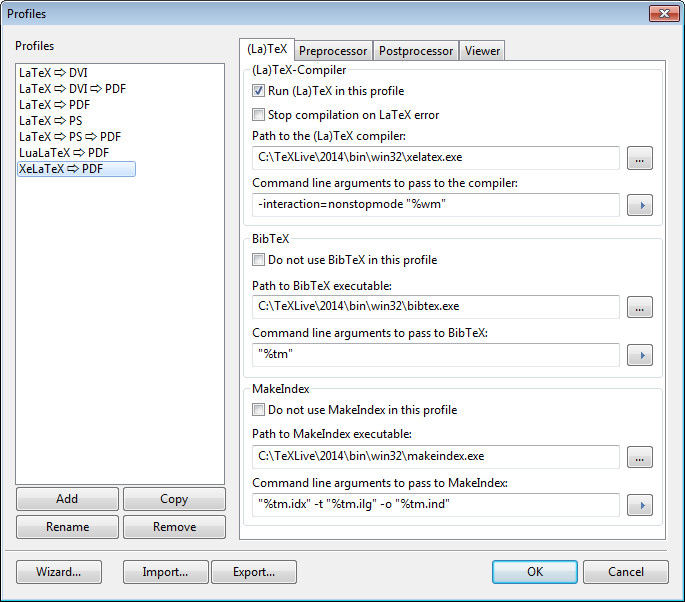
\includegraphics{images/texniccenter.jpg}}
\caption{Paramétrage de \programme{TeXnicCenter}}
\end{figure}
%%%%%%%%%%%%%%%%%%%%%%%%%%%%%%%%%%%%%%%%
%%%%%  Chapitre Liens 
%%%%%%%%%%%%%%%%%%%%%%%%%%%%%%%%%%%%%%%%

\chapter{Liens avec d'autres programmes}

\section{Conversion d'image} \index[con]{image} \label{conversionimage}

Dans le cadre de la chaîne de compilation \programme{ps2pdf} vue en page \pageref{compilations}, \LaTeX\ n'accepte que des images au format \dextension{eps}. Pour convertir un fichier image en fichier \dextension{eps}, de nombreux programmes sont disponibles. En voici un exemple avec le logiciel libre \programme{The Gimp}\footnote{Il est téléchargeable à l'adresse \liensimple{http://www.gimp.org/}.}.

Après avoir ouvert une image éditable avec \programme{The Gimp}, il faut aller dans le menu \vue{Fichier}, \vue{Exporter...} et le formulaire suivant apparaît. 

\begin{figure}[H]
\centering
\resizebox{9cm}{!}{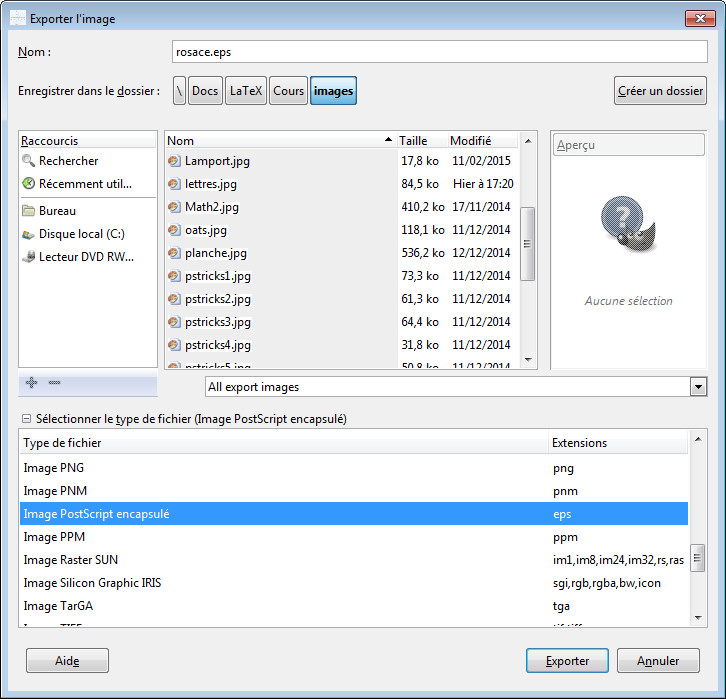
\includegraphics{images/thegimp1.jpg}}
\caption{Formulaire d'exportation de \programme{The Gimp}}
\end{figure}

Il suffit alors de changer le type de l'image en cliquant sur \vue{Sélectionner le type de fichier} puis \vue{Image postscript encapsulé} et enfin \vue{Exporter}. Dans la plupart des cas, les options proposées par défaut dans le second formulaire qui apparaît ne sont pas à modifier.

\begin{figure}[H]
\centering
\resizebox{8cm}{!}{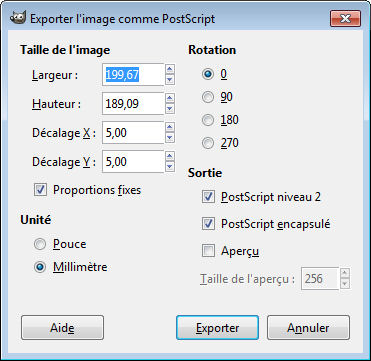
\includegraphics{images/thegimp2.jpg}}
\caption{Formulaire des options \dextension{eps} de \programme{The Gimp}}
\end{figure}

La figure s'insère alors dans \LaTeX\ en suivant la logique présentée en section \ref{images}.

\section{\programme{Excel}}

Comme vu en \ref{macroexcel} page \pageref{macroexcel}, la macro complémentaire \programme{Excel2LaTeX} permet de convertir une zone d'une feuille \programme{Excel} en un code \LaTeX\ générant un tableau simple.

Mais la transmission d'information entre \programme{Excel} et \LaTeX\ peut aller plus loin. \LaTeX\ travaille en effet sur des fichiers en format texte, format générable et manipulable par la plupart des langages de programmation, tel le \programme{Visual Basic}. Voici donc un exemple de code \programme{Visual Basic} permettant ceci :

\begin{codesimple}{Macro VB créant un code \LaTeX\ en encodage latin1}{macrovb}
Sub Test()
Open "C:\Test\liste.tex" For Output As #1
Avertissement = Cells(1, 1)
Signature = Cells(2, 1)
Print #1, "Attention :"
Print #1, "\begin{center}"
Print #1, Avertissement
Print #1, "\textsc{" & Signature & "}"
Print #1, "\end{center}"
Close #1
End Sub
\end{codesimple}

La procédure \macron{Test}, avec la commande \macron{Open For Output As \#1}, va accéder en mémoire au fichier \vue{liste.tex} dans le répertoire indiqué. Si le fichier n'existe pas, Excel le crée\footnote{Mais si le répertoire n'existe pas, \programme{Excel} ne le crée ici pas.}. Ce code récupère avec les deux lignes suivantes les valeurs présentes dans deux cellules de la feuille \programme{Excel} active. Chaque ligne commençant par \macron{Print \#1,} insère alors la suite de la ligne dans le fichier \vue{liste.tex}. La commande \vue{Close \#1} referme enfin le fichier \vue{liste.tex}.

Les différentes lignes commençant par \macron{Print \#1,} insèrent des chaînes de caractère encadrées par le caractère \macron{"} ou des variables. La concaténation de chaînes de caractère ou de variables se fait avec le caractère \macron{\&}\footnote{Ceci est vrai dans le code \programme{Visual Basic} tout comme dans les formules apparaissant dans une feuille \programme{Excel}.}.

Le fichier \vue{liste.tex} peut alors être compilé avec \LaTeX\ s'il est complet ou être intégré dans un autre fichier avec les commandes \macro{include} ou \macro{input}, comme indiqué en section \ref{scission}, page \pageref{scission}.

Pour travailler en UTF8, le code à retenir est plus complexe (mais aussi plus général) :

\begin{codesimple}{Macro VB créant un code \LaTeX\ en encodage UFT8}{macrovbutf8}
Sub Test()
' On teste l'existence du fichier final (pour le supprimer)
Set objFSO = CreateObject("Scripting.FileSystemObject")
If objFSO.FileExists("C:\Test\liste.tex") Then Kill ("C:\Test\liste.tex")
    
' Creation de l'objet contenant le texte LaTeX
Dim objStream As Object                       ' Définition
Set objStream = CreateObject("ADODB.Stream")  ' Création
objStream.Open                                ' Ouverture
objStream.Position = 0                        ' On se place au début
objStream.Charset = "UTF-8"                   ' Encodage UTF8
    
Avertissement = Cells(1, 1)
Signature = Cells(2, 1)    
objStream.WriteText "Attention :" & vbCr
objStream.WriteText "\begin{center}" & vbCr
objStream.WriteText Avertissement & vbCr
objStream.WriteText "\textsc{" & Signature & "}" & vbCr
objStream.WriteText "\end{center}" & vbCr

' Sauvegarde finale et fermeture de l'objet créé
objStream.SaveToFile "C:\Test\liste.tex"
objStream.Close
End Sub
\end{codesimple}

Ici, le \macron{vbCr} permet d'insérer un retour à la ligne.

\section{Les logiciels mathématiques}

La précision de \LaTeX\ en matière de mathématiques en a fait un des outils les plus appréciés des mathématiciens. Aussi, de nombreuses applications mathématiques proposent la génération de codes ou de figures réutilisables immédiatement par \LaTeX.


\subsection{\programme{R}, avec \programme{Sweave}}

L'extension \programme{Sweave} du logiciel \programme{R} permet de créer un document \dextension{tex} sur la base d'un document d'extension dédiée \dextension{Snw} (ou \dextension{Rnw}) placé dans le répertoire de travail usuel de \programme{R}. Ce document contient du code \LaTeX\ classique mais peut contenir aussi du code \programme{R} en respectant la norme suivante :

\begin{codesimple}{Encadrement d'un code \programme{R} sous \LaTeX}{encadrer}
<<§oc paramètres d'affichage §fc >>= 
§oc Lignes de code R §fc
@
\end{codesimple}


En voici quelques exemples appliqués :

\begin{codesimple}{Exemples de code \programme{R} sous \LaTeX}{exempler}
<<>>=  
library(stats)
x <- rnorm(20)
print(x)
print(t1 <- t.test(x))
@ 

<<echo=TRUE,print=TRUE>>= 
1 + 1          
1 + pi        
sin(pi/2) 
@
\end{codesimple}


Sous \programme{R}, ce document est exécutable avec \programme{Sweave} en utilisant la série de commandes suivantes :

\begin{codesimple}{Instructions sous \programme{R}}{instructionsr}
test <- system.file("Sweave", "§oc fichier§fc£¤.Snw", package = "utils")  \\
Sweave(test)
\end{codesimple}


Une fois que \programme{R} a effectué son traitement, il restitue un fichier \dextension{tex} et autant d'images \dextension{pdf} ou d'images \dextension{eps}\footnote{Pour obtenir des images \dextension{eps}, le fichier \dextension{Snw} doit contenir l'instruction \macro{SweaveOpts\{eps=true\}}.} que de figures demandées à \programme{R}. Le document \LaTeX\ doit contenir dans son préambule l'appel suivant :

\begin{codesimple}{Paquet nécessaire pour travailler avec \programme{R} et \programme{Sweave}}{sweave}
\usepackage{Sweave}
\end{codesimple}


Le paquet \paquet{Sweave} se trouve dans les répertoires de \programme{R} et peut être copié dans le même répertoire que votre fichier \dextension{tex}. La suite revient à l'utilisation classique de \LaTeX.

Les possibilités sont ici nombreuses et, pour une vision bien plus complète, il existe un document de Jean Raymond \textsc{Lobry}\cite{lobr} sur la question.

%%%%%%%%%%%%%%%%%%%%%%%%%%%%%%%%%%%%%%%%
%%%%%  Chapitre CV
%%%%%%%%%%%%%%%%%%%%%%%%%%%%%%%%%%%%%%%%

\chapter{Un CV sous \LaTeX}
\label{moderncv}
Pour obtenir un CV de qualité, le paquet qui sort actuellement du lot est \paquet{moderncv} de Xavier \textsc{Danaux}. Ce paquet est documenté par des exemples et le cours ci-dessous reprend ce point pour permettre à tout à chacun d'y trouver de quoi faire. Le seul point non détaillé ici est la possibilité de faire le courrier avec le CV, le courrier étant proposé dans un format anglais.


\section{Une nouvelle classe}

Le paquet \paquet{moderncv} définit tout d'abord une nouvelle classe de document nommée \macron{moderncv}. Cette dernière réagit de façon similaire aux options que sont \macron{10pt}, \macron{11pt}, \macron{12pt}, \macron{landscape}, \macron{a4paper}, \macron{a5paper} pour les plus courantes. Elle ajoute les deux options \macron{roman} et \macron{sans} qui permettent de rédiger respectivement en fonte romaine et en fonte linéale.


\section{Différents thèmes}

Ce paquet propose différents thèmes. Pour sélectionner son thème, il faut recourir à la commande \macro{moderncvtheme[{\it couleur}]\{{\it nom du thème}\}}. 
Le thème est à choisir parmi les valeurs suivantes : \macron{banking}, \macron{casual}, \macron{classic} et \macron{oldstyle}.

La \emph{couleur} est à choisir par défaut parmi les valeurs : \macron{black}, \macron{blue}, \macron{green}, \macron{grey}, \macron{orange}, \macron{purple} et \macron{red}.

Les couleurs peuvent éventuellement être redéfinies directement avec le bloc de commandes suivantes. Le bloc ci-dessous reprend le code pour obtenir l'option \macron{blue} indiquée ci-dessus\footnote{Ce bloc correspond à ce que font les différents appels d'options et qui se retrouvent dans les fichiers \macron{moderncvcolor....sty}.}.

\begin{codesimple}{Définition de couleur pour le CV}{defcoulcv}
\definecolor{color0}{rgb}{0,0,0}           % noir
\definecolor{color1}{rgb}{0.22,0.45,0.70}  % bleu clair
\definecolor{color2}{rgb}{0.45,0.45,0.45}  % gris
\end{codesimple}


La couleur \macron{color0} joue sur le texte, \macron{color1} sur les règles et les titres de section et \macron{color2} sur les coordonnées, l'encadrement de la photo et le nom.


\section{Paramètres personnels}

Différentes  commandes placées dans le préambule du document sont créées pour stocker les coordonnées obligatoires de l'auteur du CV :
\begin{itemize}
\item \macro{firstname\{{\it prénom}\}} définit le \emph{prénom} ; 
\item \macro{familyname\{{\it nom}\}} définit le \emph{nom}.
\end{itemize}

Des commandes optionnelles sont également disponibles :
\begin{itemize}
\item \macro{title\{{\it titre}\}} définit le \emph{titre} du CV ;
\item \macro{address\{{\it adresse}\}\{{\it code postal, ville}\}} définit l'adresse en deux champs ;
\item \macro{phone\{{\it numéro}\}} définit le \emph{numéro} de téléphone fixe ;
\item \macro{mobile\{{\it numéro}\}} définit le \emph{numéro} de téléphone mobile ;
\item \macro{fax\{{\it numéro}\}} définit le \emph{numéro} de fax ;
\item \macro{email\{{\it mail}\}} définit l'adresse \emph{mail} ;
\item \macro{homepage\{{\it page web}\}} définit l'adresse d'une \emph{page web} ;
\item \macro{extrainfo\{{\it infos}\}} définit des \emph{données} complémentaires ;
\item \macro{quote\{{\it citation}\}} définit une citation ; 
\item \macro{photo[{\it dimension}][{\it marge}]\{{\it image}\}} définit une photo de hauteur \emph{dimension} avec une marge d'épaisseur \emph{marge}. Il doit s'agir du nom de l'\emph{image}, \dextension{eps} ou \dextension{jpg} selon la chaîne de compilation retenue, sans indiquer l'extension. 
\end{itemize}


\section{Découpage du CV}

La partie en-tête (prénom, nom) et la partie pied de page sont générées automatiquement avec la commande \macro{makecvtitle} placée dans le corps du document. Le découpage du CV reste par contre à la main du rédacteur. La découpe du CV en différents thématiques se fait par les commandes \macro{section\{\}} et \macro{subsection\{\}}. Les différentes lignes du CV peuvent être formatées spécifiquement de quatre façons :
\begin{itemize}
\item \macro{cvitem\{{\it texte court}\}\{{\it texte long}\}}\footnote{Elle est aussi nommée \macro{cvline}.} met l'argument \emph{court} en valeur (gras ou en colonne), l'argument long étant mis à côté pour donner des détails ; 
\item \macro{cvdoubleitem\{{\it court}\}\{{\it long}\}\{{\it court}\}\{{\it long}\}}\footnote{Elle est aussi nommée \macro{cvcomputer}.} reprend l'idée de \macro{cvline} mais en traitant deux entrées en même temps par un jeu de double colonne ;
\item \macro{cvitemwithcomment\{{\it court}\}\{{\it long}\}\{{\it droite}\}}\footnote{Elle est aussi nommée \macro{cvlanguage}.} rajoute un élément placé sur la même ligne à \emph{droite} des deux premiers ;
\item \macro{cventry\{{\it dates}\}\{{\it court}\}\{{\it société}\}\{{\it ville}\}\{{\it pays}\}\{{\it long}\}} structure encore plus l'information. Elle est à réserver pour le détail des expériences ou des formations. \\
\end{itemize}

En parallèle, des commandes d'énumération sont proposées par ce paquet :
\begin{itemize}
\item \macro{cvlistitem\{{\it donnée}\}} ;
\item \macro{cvlistdoubleitem\{{\it donnée 1}\}\{{\it donnée 2}\}} propose la même énumération mais sur deux colonnes.
\end{itemize}


\section{Commandes complémentaires}

L'observation de plusieurs exemples d'utilisation de \paquet{moderncv} montre qu'il est souvent fait appel aux deux commandes suivantes dans le préambule du document pour affiner la présentation du CV :
\begin{itemize}
\item \macro{usepackage[scale=0.8]\{geometry\}} afin de régler les dimensions du CV par rapport à la feuille de papier par l'appel de \paquet{geometry} ;
\item \macro{nopagenumbers\{\}} qui empêche la numérotation des pages du CV.
\end{itemize}


\section{Exemple}

\begin{codesimple}{Exemple de CV}{exemplecv}
\documentclass[10pt,a4paper]{moderncv}
\moderncvtheme[blue]{oldstyle}
\usepackage[scale=0.8]{geometry}
\firstname{Garfield}
\familyname{Lechat}
\title{Chat domestique}
\address{8 rue Lasagne}{Cheshire}
\photo[64pt]{garfield}

\begin{document} 
\makecvtitle

\section{Expériences}
\cventry{2010}{Testeur de matelas}{Dodo}{Le Mans}{France}{}
\cventry{2008--2009}{Coinceur de bulle}{Sommeil blanc}{Poitiers}{France}{}

\end{document}
\end{codesimple}


\section{Pour aller plus loin}

Parmi les autres modèles de CV qui peuvent être trouvés sur l'Internet, citons ici :
\begin{itemize}
\item celui d'Olivier \textsc{Bichler}\footnote{\liensimple{http://olivier.bichler.free.fr/www/?page=content/index&blog_content_articleId=26}.} utilisant une classe permettant de faire un CV avec contenu optionnel ;
\item celui d'Adrien \textsc{Friggeri}\footnote{\liensimple{https://github.com/afriggeri/CV}.}, très graphique, utilisant une classe se basant en particulier sur les fonctionnalités de \XeLaTeX\ et \paquet{tikz}.
\item le site \emph{\LaTeX\ templates}\cite{temp} propose également de nombreuses autres maquettes toutes aussi intéressantes\footnote{\liensimple{http://www.latextemplates.com/cat/curricula-vitae}.}.
\end{itemize}

%%%%%%%%%%%%%%%%%%%%%%%%%%%%%%%%%%%%%%%%
%%%%%  Chapitre Page de garde
%%%%%%%%%%%%%%%%%%%%%%%%%%%%%%%%%%%%%%%%

\chapter{La page de garde} \label{pagedegarde}
\section{Définition et exemple}

L'extension \paquet{pagedegarde} permet d'inclure dans un document \LaTeX{} la page de garde \og officielle \fg de l'\ia déclinée avec les spécificités de chaque filière, telle qu'elle apparaît ci-après sur un exemple pour l'ISUP.

Voici un exemple de code permettant de la générer. Les appels d'extensions usuelles de début de document n'y sont pas indiquées.\\

\begin{codesimple}{Exemple de génération de la page de garde}{exemplepagedegarde}
\documentclass[a4paper,11pt,twoside]{article}
\usepackage[frenchb]{babel} 
\usepackage[T1]{fontenc}
\usepackage[latin1]{inputenc} 
\usepackage{lmodern}

\usepackage[confiun,hyperref,isup]{pagedegarde}

\dategarde{22 février 1963}
\auteurgarde{Jean}{Dieudonné}
\titregarde{Tentative de définition systématique d'une §oc (...) §fc}
\juryiagarde{Nicolas}{Bourbaki}
\juryagarde{Carl Friedrich}{Gauss}
\jurybgarde{David}{Hilbert}
\directeurgarde{Pierre-Simon}{de Laplace}
\invitegarde{Jean Baptiste Joseph}{Fourier}

\begin{document}
\pagedegarde
§oc  Le reste du document... §fc 
\end{document}
\end{codesimple}


Ce code est fourni dans le fichier \macron{testdegarde.tex} qui accompagne cette documentation, le fichier d'extension \macron{pagedegarde.sty} et les images dans leur répertoire dédié (répertoire dont le nom ne doit pas être modifié).

% Insertion de la page "pagedegarde"
\newpage
\setcounter{pagetempo}{\value{page}} % Stockage du numéro de page
\pagedegarde                         % Affichage de la page 
\setcounter{page}{\value{pagetempo}} % Récupération de l'ancien numéro de page
\addtocounter{page}{1}               % Et enfin ajout d'un au numéro.
% Fin de l'insertion


\section{Appel de l'extension}

L'extension \paquet{pagedegarde} est munie de plusieurs options permettant d'effectuer des réglages de la présentation de la page de garde. L'appel avec option se fait sous la forme suivante : 
\begin{center}
\macro{usepackage[\textit{option1},\textit{option2},...]\{pagedegarde\}}
\end{center}

Il est recommandé de charger cette extension plutôt en fin de préambule du document. En effet, elle charge par défaut les extensions suivantes : \paquet{ifpdf}, \paquet{xcolor} (avec son option \macron{dvipsnames}), \paquet{graphicx}, \paquet{xspace} et \paquet{geometry}. Elle peut également, par le biais des options, charger l'extension \paquet{hyperref}, cette dernière devant normalement être la dernière chargée.

\subsection{L'option de filière}

Par défaut, le document est considéré comme un mémoire sans filière : seul le logo de l'IA apparaît et il est évoqué le terme de \og filière \fg{}. Un choix d'option doit être effectué pour modifier les affichages par défaut.

Trois filières sont définies: 
\begin{itemize}
\item l'EURIA avec l'option \macron{euria} ;
\item l'EURIA en lien avec Télécom Bretagne avec l'option \macron{telecomb} ;
\item l'ISUP avec l'option \macron{isup}.
\end{itemize}

\subsection{L'option de brouillon}

Par défaut, le document est présenté en mode finalisé. Un mode brouillon est cependant disponible par le biais de l'option \macron{draft}. Il permet d'observer les différents champs paramétrables en gris. Si ces champs n'ont pas valeur, \paquet{pagedegarde} affiche alors la commande permettant de remplir ce champ à l'endroit où il sera affiché.


\subsection{Les options de confidentialité}

Par défaut, le document est considéré comme non confidentiel. Pour spécifier une durée de confidentialité, cinq options sont disponibles selon la durée de confidentialité : 
\begin{itemize}
\item \macron{confiun} : un an ;
\item \macron{confideux} : deux ans ;
\item \macron{confitrois} : trois ans ;
\item \macron{confiquatre} : quatre ans ;
\item \macron{conficinq} : cinq ans.
\end{itemize}


\subsection{L'option de page verso uniquement}

Par défaut, le verso de la page de garde reste totalement vide, présentation usuelle pour un document en recto-verso. Ce comportement peut être modifié en spécifiant l'option \macron{versoseul}. La page suivant immédiatement la page de garde est alors accessible.


\subsection{L'option de liens hypertextes}

L'option \macron{hyperref} charge l'extension \paquet{hyperref} gérant les liens hypertextes dans les documents PDF. Sur la page de garde, les sigles ainsi que les noms des filères et autres organismes renvoient alors vers les sites internet associés.

L'utilisation de cette option sélectionne certains réglages de l'extension \paquet{hyperref} et ceci peut influer sur la présentation de l'ensemble du document. Il faut donc ici spécifier après le chargement de l'extension \paquet{pagedegarde} les options nécessaires à l'extension \paquet{hyperref} pour présenter le reste du mémoire. Ceci s'obtient avec la  commande \macro{hypersetup\{{\it options}\}}, les \emph{options} étant celles qui se retrouvent pour l'appel du paquet \paquet{hyperref}.

\section{Paramètres}

Les champs paramétrables de la page de garde sont alimentés par différentes  commandes. La liste en est la suivante :


\begin{table}[H]
\centering
\begin{tablecouleur}
\begin{tabular}{cc}
\rowcolor{bleu20}
\color{white}\bf Commande	
& \color{white}\bf Affichage					    			 	\\ 
\macro{dategarde\{{\it date}\}}
& Date de la présentation du mémoire	
\\
\macro{auteurgarde\{{\it prénom}\}\{{\it nom}\}}		
& Identité de l'auteur du mémoire
\\
\macro{titregarde\{{\it titre}\}}						
& Titre du mémoire
\\
\macro{juryiagarde\{{\it prénom}\}\{{\it nom}\}}
& Identité du jury IA
\\
\macro{juryagarde\{{\it prénom}\}\{{\it nom}\}}
& Identité du 1\ier jury filière
\\
\macro{jurybgarde\{{\it prénom}\}\{{\it nom}\}}	
& Identité du 2\ieme jury filière
\\
\macro{jurycgarde\{{\it prénom}\}\{{\it nom}\}}
& Identité du 3\ieme jury filière
\\
\macro{jurydgarde\{{\it prénom}\}\{{\it nom}\}}
& Identité du 4\ieme jury filière
\\
\macro{juryegarde\{{\it prénom}\}\{{\it nom}\}}
& Identité du 5\ieme jury filière
\\
\macro{juryfgarde\{{\it prénom}\}\{{\it nom}\}}
& Identité du 6\ieme jury filière
\\
\macro{directeurgarde\{{\it prénom}\}\{{\it nom}\}}
& Identité du directeur de mémoire
\\
\macro{invitegarde\{{\it prénom}\}\{{\it nom}\}}
& Identité de l'invité
\\
\macro{entreprisegarde\{{\it entreprise}\}}
& Entreprise associée au mémoire
\end{tabular}
\end{tablecouleur}
\caption{Les paramètres de \pseudopaquet{pagedegarde}}
\end{table}

\section{Affichage}

L'affichage de la page de garde est obtenu en plaçant la commande \macro{pagedegarde} à l'endroit souhaité dans le corps du document.  Aussi, cette page pourrait donc être placée n'importe où dans le document.

Dans l'exemple de code présenté au début de ce document, la position de la commande correspond à la position la plus naturelle : elle produit la page de garde en toute première page.


\section{Commandes complémentaires} \label{fonctionscomp}

L'extension \paquet{pagedegarde} crée quelques commandes spécifiques aux organismes cités dans la page. Ces commandes sont ainsi toutes réutilisables.


\subsection{Commandes de texte}

Cinq commandes écrivant du texte sont mises à disposition :

\begin{table}[H]
\centering
\begin{tablecouleur}
\begin{tabular}{cc}
\rowcolor{bleu20}
\color{white}\bf Commande	& \color{white}\bf Affichage	\\ 
\macro{EURIA} 				& \EURIA  						\\
\macro{Euria}				& \Euria						\\
\macro{euria}				& \euria						\\
\macro{euriamail}			& \euriamail					\\
\macro{ia}					& \ia							\\
\macro{ISUP}				& \ISUP							\\
\end{tabular}
\end{tablecouleur}
\caption{Commandes complémentaires de texte de \pseudopaquet{pagedegarde}}
\end{table}

\subsection{Commandes de sigle}

Quelques commandes sont mises à disposition pour afficher des sigles hors de la page de garde. Tous les sigles sont conditionnés à l'affichage par une dimension.

\begin{table}[H]
\centering
\begin{tablecouleur}
\begin{tabular}{cc}
\rowcolor{bleu20}
\color{white}\bf Commande					& \color{white}\bf Affichage	\\ 
\macro{euriasigle\{{\it dimension}\}}		& Sigle de l'EURIA				\\
\macro{iasigle\{{\it dimension}\}} 			& Sigle de l'IA					\\
\macro{isupsigle\{{\it dimension}\}} 		& Sigle de l'ISUP				\\
\macro{telbsigle\{{\it dimension}\}}		& Sigle de Télécom Bretagne		\\
\macro{ubosigle\{{\it dimension}\}}			& Sigle de l'UBO				\\
\end{tabular}
\end{tablecouleur}
\caption{Commandes complémentaires de sigle de \pseudopaquet{pagedegarde}}
\end{table}

Voici les différents sigles :
\begin{figure}[H]
\centering
\euriasigle{1cm} \\[1em]
\iasigle{2.5cm} \quad \isupsigle{2.5cm} \quad \telbsigle{2.5cm} \quad \ubosigle{2.5cm}
\caption{Sigles}
\end{figure} 

Le sigle de l'EURIA est composé d'un texte et d'une image. Le texte peut donc être affiché dans des polices de caractères différentes, la ligne colorée s'ajustant à la longueur du texte.

\subsection{Commandes avec lien hypertexte}

Si l'option \macron{hyperref} de \paquet{pagedegarde} est sélectionnée, il suffit de rajouter le suffixe \macron{ref} aux commandes vues dans cette section \ref{fonctionscomp} pour obtenir des commandes générant un lien hypertexte dans le document PDF. Par exemple :
\begin{itemize}
\item \macro{EURIA} devient \macro{EURIAref};
\item \macro{ubosigle\{{\it dimension}\}} devient \macro{ubosigleref\{{\it dimension}\}} et ainsi de suite. \\
\end{itemize}

En l'absence de cette option, ces commandes deviennent strictement équivalentes aux commandes sans le suffixe \macron{ref}.
%%%%%%%%%%%%%%%%%%%%%%%%%%%%%%%%%%%%%%%%
%%%%%  Chapitre Erreurs
%%%%%%%%%%%%%%%%%%%%%%%%%%%%%%%%%%%%%%%%

\chapter{Avant de réduire votre ordinateur en poussière} \index[con]{erreur} \label{erreur}

\section{Quelques réflexes de survie}

\subsection{Réflexes pour amateurs}

\LaTeX\ indique normalement le numéro de ligne où se situe l'anomalie qui l'empêche de compiler le document. Toutefois, ce numéro de ligne peut parfois être faux ! La recherche des erreurs peut alors se faire en déplaçant dans le document la commande \macro{end\{document\}} puis compiler. Ceci permet de déterminer, après quelques essais, quelle partie du code ou quelle ligne de code crée l'anomalie de compilation.

Certaines erreurs peuvent également survenir à retardement car elles peuvent être transmises aux fichiers réutilisés par \LaTeX\ lors des compilations suivantes comme \dextension{aux}, \dextension{ind}... Ce cas est souvent délicat à analyser. Aussi, si une erreur se produit sans raison apparente, la suppression des fichiers générés par la compilation peut parfois aider à résoudre le problème\footnote{Il s'agit souvent de la dernière opération de correction d'une erreur... qui, si elle échoue, conduit à donner des coups de tête au premier mur qui passe.}. 

\subsection{Réflexes pour passionnés}

\LaTeX\ dispose de primitives lui permettant de décrire de façon beaucoup plus détaillée les travaux qu'il exécute :
\begin{itemize}
\item \macro{tracingcommands=1} (ou 2) affiche le détail des commandes utilisées, le chiffre précisant la profondeur de l'analyse effectuée ; 
\item \macro{tracingall} affiche beaucoup plus d'informations que la première commande en restituant dans le fichier journal le contenu des pages, les définitions et redéfinitions que \LaTeX\ opère.  
\end{itemize}

Ces analyses demandent une connaissance de \LaTeX\ assez avancée. Les lecteurs intéressés pourront lire à profit la très complète annexe B de \cite{gomi}\footnote{Disponible en ligne : \liensimple{http://latex-project.org/guides/lc2fr-apb.pdf}.}.

\section{Le bestiaire monstrueux}

La liste qui suit présente quelques erreurs fréquemment rencontrées lors du cours. Cette liste n'est en aucun cas exhaustive : pour analyser d'autres erreurs, l'annexe B de \cite{gomi} citée à la section précédente devrait pouvoir apporter un complément d'information appréciable.

\subsubsection{Bad math environment delimiter}

Le cas survient lorsqu'un environnement mathématique a été ouvert avec la balise fermante, par exemple en écrivant \macro{]} au lieu de \macro{[}.

\subsubsection{Display math should end with \$\$}

La fermeture d'un environnement mathématique hors ligne n'a pas été faite avec la bonne commande, par exemple en mettant un \macron{\$} au lieu d'un \macro{]} après avoir mis un \macro{[}. Il est à noter que le \macron{\$\$}, pourtant suggéré ici par \LaTeX, doit être évité.

\subsubsection{Extra \}, or forgotten \$}

Le cas survient lorsqu'un environnement mathématique a été ouvert sans être refermé.

\subsubsection{File ended while scanning use of...}

Cette erreur indique qu'une accolade ouvrante n'a jamais été suivie de l'accolade fermante (\LaTeX\ allant la chercher jusqu'à la fin du fichier). Cette erreur est suivie du nom de la commande pour laquelle il manque l'accolade fermante.

\subsubsection{Missing \$ inserted}

Les commandes présentant des mathématiques requièrent un environnement mathématique. Ceci apparaît le plus souvent en présence de caractères dédiés comme \macron{\_}, \macron{\^{}}, de lettres grecques comme \macro{alpha} ou de commandes mathématiques comme \macro{sum}, ceci sans que le mode mathématique ait été appelé (avec par exemple \macron{\$} ou \macro{[}). 


\subsubsection{No room for a new...} 

Le chargement de nombreux paquets peut saturer la mémoire allouée (des registres) à \LaTeX\footnote{Voir  \liensimple{http://www.tex.ac.uk/cgi-bin/texfaq2html?label=noroom}.}. Pour contourner cette difficulté, il peut être fait usage des commandes suivantes en début de préambule, le \macron{28} étant un paramètre libre :

\begin{codesimple}{Augmentation de capacité pour \LaTeX}{capacitelatex}
\usepackage{etex}
\reserveinserts{28}
\end{codesimple}


\subsubsection{Too many \}'s} 

Fréquente en cas de formules mathématiques, cette erreur a pour source un caractère \macron{\}} en trop ou un caractère \macron{\{} manquant.


\subsubsection{Undefined control sequence} 

Normalement suivie de la commande coupable, vous vous trouvez ici face à une commande dont \LaTeX\ n'a pas la définition. Trois possibilités : 
\begin{itemize}
\item vous n'avez pas chargé le paquet définissant cette commande ;
\item vous n'avez pas défini cette commande dans le préambule ;
\item vous ne savez pas utiliser vos doigts\footnote{Vous connaissant, ce cas s'avère être le plus probable.}.
\end{itemize}


%%%%%%%%%%%%%%%%%%%%%%%%%%%%%%%%%%%%%%%%
%%%%%  Index
%%%%%%%%%%%%%%%%%%%%%%%%%%%%%%%%%%%%%%%%

\printindex[paq]
\printindex[con]


%%%%%%%%%%%%%%%%%%%%%%%%%%%%%%%%%%%%%%%%
%%%%%  Bibliographie
%%%%%%%%%%%%%%%%%%%%%%%%%%%%%%%%%%%%%%%%

\nocite{*}                             % Demande d'écriture de toutes les entrées du fichier ".bib"
\bibliographystyle{plain-fr}           % Utilisation d'un style francisé : plain-fr (http://www.lsv.ens-cachan.fr/~markey/bibla.php)
\bibliography{bibliocours}             % Appel du fichier de références


\end{document}
